% thesis.tex (starting point of a UTas mathematics thesis)

% Note that the following defaults are also contained in the 'report' class
% (this is not exhaustive...see appropriate references for all options)
% 'oneside' mode...overide with 'twoside' to force output for two-sided printing.
% 'final' mode...overide with 'draft' to see linebreak malfunctioning.
% For example, to use two-sided printing one would declare the 'documentclass'
% as follows...
% '\documentclass[11pt,a4paper,twoside]{report}'
%
% Specific Mathematical options are as follows
% 'leqno' to force equation numbering on the left side of the page.
% 'fleqn' to force formulas to flush left (centered is the default).
% If 'fleqn' is specified then the left indent is controlled with '\mathindent'.
% i.e. '\setlength{\mathindent}{2.5cm}'

% Declare overall type of document (use 11pt report class on A4 paper).
\documentclass[11pt,a4paper]{report}
% If you want to generate an index you should include the following command
% which puts a makeindex command in the preamble. Additionally, you need to un-comment
% the file 'index' in the '\includeonly' command below and also include the 'index'
% file in the main document.
\makeindex

% Include the style file which contains all the required formatting
% information that is set out in the Research Higher Degrees Resource
% Handbook (2003 version). NOTE: This file uses the following packages
% 'graphicx' for graphics manipulation
% 'fancyhdr' for nice headers and footers.
% 'makeidx' for generating the index
% 'tocbibind' for adding table of contents entries for bibliography, index etc.
% 'sectsty' for generating stylised chapter and section headings.
% You will need to make sure your LaTeX installation has these packages
% installed...else it wont work :(

% Style file to assist in generating a University
% of Tasmania PhD thesis in Mathematics. Contains all the required formatting
% options and header/footer information that is set out in the
% Research Higher Degrees Resource Handbook (2003 version)
% This file should be easily modifiable to comply with
% minor formatting changes (such as the left margin width etc.)

% First set the required page format...margins, text widths etc.
% Note 1in=2.54cm and LaTeX has a fixed border of 1in on top and left
% margins so we need to take this into account when calculating sizes.
% Set the top margin to be 1inch from the paper edge.
\setlength{\topmargin}{0.0cm}
% Set the header-body separation level
\setlength{\headsep}{1.0cm}
% Set the footskip to be 2cms
%->\setlength{\footskip}{0.1cm}
\setlength{\footskip}{0.5cm}
% Set the header height to be 1cm
\setlength{\headheight}{1cm}
% Set the bottom margin to be 1 inch from the paper edge by
% way of the \paperheight and \textheight commands
% First set up a new length called \textheit
\newlength{\textheit}
% Set the value of \textheit to the total paper height for
% the paper size declared in the \documentclass command
\setlength{\textheit}{\paperheight}
% Subtract off 1 inch from top and bottom of the paper
\addtolength{\textheit}{-2.0in}
% Subtract off the \topmargin height
\addtolength{\textheit}{-\topmargin}
% Subtract off the \headheight height
\addtolength{\textheit}{-\headheight}
% Subtract off the \headsep height
\addtolength{\textheit}{-\headsep}
% Subtract off the \footskip height
\addtolength{\textheit}{-\footskip}
% Finally, set the text height to that calculated above
\setlength{\textheight}{\textheit}
% Set the text to flush to the bottom of each page
%\flushbottom

% Set the odd and even left margins to be 4.5cm from paper edge.
% Note that 4.50cm-2.54cm=1.96cm
\setlength{\oddsidemargin}{1.96cm}
\setlength{\evensidemargin}{1.96cm}
% Set the right margin to be 1 inch from the paper edge by
% way of the \paperwidth and \textwidth commands
% First set up a new length called \textwid
\newlength{\textwid}
% Set the value of \textwid to the total paper width for
% the paper size declared in the \documentclass command
\setlength{\textwid}{\paperwidth}
% Subtract off 1 inch from each side of the paper
\addtolength{\textwid}{-2.0in}
% Subtract off the \oddsidemargin width
\addtolength{\textwid}{-\oddsidemargin}
% Finally, set the text width to that calculated above
\setlength{\textwidth}{\textwid}
% Set the paragraph spacing
\setlength{\parskip}{6pt}
% Set the paragraph indentation level
\setlength{\parindent}{0pt}


% Load the graphicx package
\usepackage{graphicx}

% Load the makeidx package for easy index generation
\usepackage{makeidx}


% Load the tocbibin package for putting in table of
% contents entries for the bibliograpy and index.
\usepackage{tocbibind}
% Set the table of contents name
\settocname{TABLE OF CONTENTS}
% Set the list of figures name
\setlofname{LIST OF FIGURES}
% Set the list if tables name
\setlotname{LIST OF TABLES}
% Set the bibliograpy name
\settocbibname{BIBLIOGRAPHY}
% Set the index name
\setindexname{INDEX}


% Load the sectsty package for generating stylised
% chapter and section headings.
\usepackage{sectsty}
% Set the Chapter font specifications
%\chapterfont{\nohang\rmfamily\centering}
% Set the Section font specifications
\sectionfont{\nohang\rmfamily\centering}
% Set the Subsection font specifications
%\subsectionfont{\nohang\rmfamily\raggedright}
% Set the Subsubsection font specifications
%\subsubsectionfont{\nohang\rmfamily\raggedright}


% Load the fancy headers package for manipulating
% the material that appears in the headers and footers.
\usepackage{fancyhdr}
\pagestyle{fancy}
% Set up the default behavior for headers and footers
\fancyhead[L]{} \fancyhead[C]{\rightmark} \fancyhead[R]{\thepage}
\fancyfoot[L]{} \fancyfoot[C]{} \fancyfoot[R]{}
% Set the header and footer rule width to 0.0pt
\renewcommand{\headrulewidth}{0pt}
\renewcommand{\footrulewidth}{0pt}


% Now take care of all the user specific entries like
% the title, author, abstract, table of contents etc.

% Use this so LaTeX can differentiate user defined commands
% from internal ones. Modifies how LaTeX interprets the @ symbol...
\makeatletter

% Set some basic lengths
\newlength{\li} \setlength{\li}{12pt}
\newlength{\signed} \settowidth{\signed}{signedd}
\newcommand{\singlespace}{\baselineskip 1.1\li}
\newcommand{\doublespace}{\baselineskip 2.0\li}

% Defines new 'if' variables for boolean checks
\newif\iftitlepg \titlepgtrue
\newif\ifsignaturepage \signaturepagetrue
\newif\ifcopyright \copyrighttrue
\newif\ifaltcopyright \altcopyrighttrue
\newif\ifabswithesis \abswithesistrue
\newif\ifack \acktrue
\newif\iftablecontents \tablecontentstrue
\newif\iftablespage \tablespagefalse
\newif\iffigurespage \figurespagetrue 



% Redefine the chapter commands for nicer formatting
\renewcommand{\@makechapterhead}[1]{%
  \vspace*{50\p@}%
  {\parindent \z@ \centering \reset@font
    \ifnum \c@secnumdepth >\m@ne
         \normalfont \LARGE \rmfamily \scshape \@chapapp{} \thechapter  % Chapter followed by number
         \par
         \vskip 20\p@
       \fi
    \normalfont \Huge \rmfamily  #1\par          % chapter title
    \nobreak
    \vskip 40\p@
  }}

\renewcommand{\@makeschapterhead}[1]{%
  \vspace*{50\p@}%
  {\parindent \z@ \centering
    \reset@font
    \normalfont \Huge \rmfamily  #1\par
    \nobreak
    \vskip 40\p@
  }}


% Helpful command for making prefaces and the like
\def\prefacesection#1{%
    {\null\vskip .50in 
    \begin{center}
        {\normalfont \Huge \rmfamily {#1 \vskip 2\li}}
    \end{center}}}

% Gets the information about the author, title etc from the file
% 'prelude.tex' and populates the relevant fields.
\def\dept#1{\gdef\@dept{#1}}
\def\advisor{\gdef\@advisor}
\def\prevdegrees{\gdef\@prevdegrees}
\def\submitdate#1{\gdef\@submitdate{#1}}
\def\copyrightyear#1{\gdef\@copyrightyear{#1}} 
\def\@title{}
\def\@author{}
\def\@dept{}
\def\@submitdate{\ifcase\the\month\or
  January\or February\or March\or April\or May\or June\or
  July\or August\or September\or October\or November\or December\fi
  \space \number\the\year}
\ifnum\month=12
    \@tempcnta=\year \advance\@tempcnta by 1
    \edef\@copyrightyear{\number\the\@tempcnta}
\else
    \def\@copyrightyear{\number\the\year}
\fi

% Command to make the title page
\def\titlepg{%
    \newpage
    \pagenumbering{roman}
    \thispagestyle{empty}%
    \singlespace
        \null\vskip0.25in
    \begin{center}
        {\Large\uppercase\expandafter{\@title}}
    \end{center}
    \null\vskip0.25in
    \begin{center}
       \rm  by\\
    \end{center}
    \null\vskip0.25in
    \begin{center}
       \rm \large\@author , \@prevdegrees\\
    \end{center}
    \null\vskip0.5in
    \begin{center}
           {\rm 
                \vskip \li 
            Submitted in fulfilment of the requirements \\
            for the Degree of Doctor of Philosophy\\}
    \end{center}
    \null\vskip1.0in
    \begin{center}
          {\rm \large Department of {\@dept}\\
          University of Tasmania\\
          {\@submitdate} \\
          \null\vskip0.25in
          \begin{figure*}[hbtp]
          \begin{center}
          \scalebox{.30}{
\includegraphics{Utas_vert_BW}}
          \end{center}
          \end{figure*}}
    \end{center}
    \vfill}

% Command to make the declaration of originality
\def\signaturepage{%
    \newpage
    \null\vfill
    \thispagestyle{empty}%
    \begin{quote}
        {\normalsize I declare that this thesis contains no material
          which has been accepted for a degree or diploma by the
          University or any other institution, except by way of
          background information and duly acknowledged in the thesis,
          and, to the best of my knowledge and belief, no material
          previously published or written by another person, except
          where due acknowledgement is made in the text of the thesis;
          nor does the thesis contain any material that infringes
          copyright. }

    \end{quote}
    \null\vskip0.5in
    \begin{quote}
    {Signed:  \hrulefill \hfill \hfill
        \newline\hspace*{\signed} \raisebox{4.0mm}{\@author}
        \newline
        Date:  \hrulefill \hfill \hfill \hfill}
    \end{quote}
    \vskip 1.0in
    \vfill}

% Command to make the copyright page
\def\copyrightpage{%
    \newpage
    \null\vfill
    \thispagestyle{empty}%
    \begin{quote}
        {\normalsize This thesis may be made available for loan and limited copying in 
        accordance with the {\sl Copyright Act 1968}}
    \end{quote}
    \null\vskip0.5in
    \begin{quote}
    {Signed:  \hrulefill \hfill \hfill
        \newline\hspace*{\signed} \raisebox{4.0mm}{\@author}
        \newline
        Date:  \hrulefill \hfill \hfill \hfill}
    \end{quote}
    \vskip 1.0in
    \vfill}

% Command to make the copyright page
\def\altcopyrightpage{%
    \newpage
    \null\vfill
    \thispagestyle{empty}%
    \begin{quote}
        {\normalsize The publishers of papers comprising Chapters 2
          and 4 hold the copyright for those chapters, and access to
          the material should be sought from the respective journals.
          The remaining non-published content of the thesis may be
          made available for loan and limited copying and
          communication in accordance with the {\sl Copyright Act
            1968}}
    \end{quote}
    \null\vskip0.5in
    \begin{quote}
    {Signed:  \hrulefill \hfill \hfill
        \newline\hspace*{\signed} \raisebox{4.0mm}{\@author}
        \newline
        Date:  \hrulefill \hfill \hfill \hfill}
    \end{quote}
    \vskip 1.0in
    \vfill}

% Command to make the abstract page
\def\abswithesis{
    \newpage
    % Set up the default behavior for headers and footers
    \thispagestyle{empty}
    \prefacesection{ABSTRACT}
    \abstextwithesis
}


% Command to make the acknowledgements page
\def\ackpage{
    \newpage
    % Set up the default behavior for headers and footers
    \thispagestyle{empty}
    \prefacesection{ACKNOWLEDGEMENTS}
    \acknowledgement
}


% Sets up all the stuff before the table of contents.
\def\beforepreface{
\iftitlepg\titlepg\fi
\ifsignaturepage\signaturepage\fi
\ifcopyright\copyrightpage\fi
\ifaltcopyright\altcopyrightpage\fi
\ifabswithesis\abswithesis\fi
\ifack\ackpage\fi
}

% Takes care of the table of contents, figures etc 
\def\afterpreface{
\pagestyle{fancy}
\setcounter{page}{0}
\iftablecontents\tableofcontents\fi
\iftablespage\listoftables\fi
\iffigurespage\listoffigures\fi
}

% Reset the behaviour of the @ symbol
\makeatother


%\let\chapter\section

%\usepackage{accents}
%\usepackage{algorithm2e}
%\usepackage{frankenstein}
%\usepackage{graphicx}
%\usepackage{slashed}
\usepackage{a4}
\usepackage{esvect}
\usepackage[OT1]{fontenc}
\usepackage{outline}
\renewcommand*\familydefault{ocm}
\usepackage[outline]{contour}
\usepackage{algorithm}
\usepackage{algpseudocode}
\usepackage{amsmath}
\usepackage{stmaryrd}
\usepackage{amssymb}
\usepackage{amsthm}
\usepackage{enumitem}
\usepackage{lmodern}
\usepackage{mathtools}
\usepackage{url,lineno}
\usepackage{graphicx}
\usepackage{pdflscape}
\usepackage{listings}
%%\usepackage{color}
\usepackage[usenames]{xcolor}
\usepackage{textcomp}
\usepackage{accents}
\lstset{
  language=Scheme
}


\usepackage[authoryear]{natbib}
%% \usepackage[
%%     backend=bibtex,
%%     style=authoryear-icomp,
%%     sortlocale=en_AU,
%%     natbib=true,
%%     url=false, 
%%     doi=true,
%%      eprint=false
%% ]{biblatex}
%
 %%%%\addbibresource{biblatex-examples.bib}
 %%\usepackage[]{hyperref}
%%\setcitestyle{authoryear, open={((},close={))}


%-- Fonts
%\usepackage[T1]{fontenc}
\usepackage{calligra}
%%\usepackage{chancery}

\DeclareGraphicsExtensions{.eps,.pdf,.png}

\DeclareMathAlphabet{\mathocm}{OT1}{ocm}{m}{rm}
\DeclareMathAlphabet{\mathsfsl}{OT1}{cmss}{m}{sl}
\DeclareMathAlphabet{\mathpzc}{OT1}{pzc}{m}{it}


\typeout{Got packages}

% Here you would include any additional packages that you want to use.
% You should make sure they don't clash with the above packages that
% are in use in the style file.

% Specify which pieces (other .tex files) you plan to include. You can comment
% out files that you will include later or have already finished to speed
% up TeX processing
%% \includeonly{
%% prelude % Contains all the relevant candidate information (name, degrees, abstract etc)
%% ,newcom % Place all you new commands in here
%% ,chap1  % Introduction
%% ,chap2  % paper 1
%% ,chap3  % Definitions, proofs
%% ,chap4  % paper 2
%% ,chap5  % explicit model
%% ,concl  % conclusion ... of course
%% ,app0   % code for explicit model
%% ,app1   % limited results
%% ,biby   % Makes the bibliography from the BibTeX database
%% ,index  % Places the index in the thesis
%% }


\typeout{Starting document}

% Include all the pieces of your thesis in here.
% prelude.tex (specification of which features in `mathphdthesis.sty' you
% are using, your personal information, and your title & abstract)

% Specify features of `mathphdthesis.sty' you want to use:
\titlepgtrue % main title page (required)
\signaturepagetrue % page for declaration of originality (required)
%\copyrighttrue % copyright page (required)
\altcopyrighttrue % copyright page (required)
\abswithesistrue % abstract to be bound with thesis (optional)
\acktrue % acknowledgments page (optional)
\tablecontentstrue % table of contents page (required)
\tablespagetrue % table of contents page for tables (required only if you have tables)
\figurespagetrue % table of contents page for figures (required only if you have figures)

\title{ADAPTIVE SIMULATION MODEL CONFIGURATION} % use all capital letters
\author{Randall Gray} % use mixed upper & lower case
\prevdegrees{B.A. (Flinders University of South Australia)} % Used to specify your previous degrees...use mixed upper & lower case
\advisor{Dr Simon Wotherspoon} % example: Professor Lawrence K. Forbes
\dept{Mathematics} % your academic department
\submitdate{October, 2016} % month & year of your thesis submission

\typeout{******* in manifest.tex}
%% \newcommand{\blockcomment}[1]{}
%% \newcommand{\UseFirstVersion}[2]{#1}
%% \newcommand{\UseSecondVersion}[2]{#2}
%% \newcommand{\UseNeitherVersion}[2]{}



\typeout{bungie jumping}
\iftoggle{usesMnSymbol}{
   \typeout{using MnSymbol}
   \newcommand{\BBN}[0]{\mathbb{N}}
   \newcommand{\BBNO}[0]{\mathbb{N}^0}
   \newcommand{\BBNI}[0]{\mathbb{N}^+}
   \newcommand{\mB}[1]{\mathbb{#1}}
   \newcommand{\dotcup}{\ensuremath{\mathaccent\cdot\cup}}
}{
   \typeout{Hack the barstud}
   \DeclareMathAlphabet{\mathoss}{OT1}{cmss}{m}{sl}
   \DeclareMathAlphabet{\mathsfsl}{OT1}{cmss}{m}{sl}
   \typeout{declaring BBN BBNO BBNI mB ranglebar langlebar dotcup}
   \newcommand{\BBN}[0]{\mathbb{N}}
   \newcommand{\BBNO}[0]{\mathbb{N}^0}
   \newcommand{\BBNI}[0]{\mathbb{N}^+}
   \newcommand{\mB}[1]{\mathbb{#1}}
   \newcommand{\ranglebar}{\lvert\rangle}
   \newcommand{\langlebar}{\langle\rvert}
   \newcommand{\dotcup}{\ensuremath{\mathaccent\cdot\cup}}
}

\newcommand{\mt}[1]{\mathtt{#1}}
\newcommand{\ms}[1]{\mathsf{#1}}
\newcommand{\mb}[1]{\boldsymbol{#1}}  %% from amsbsy
\newcommand{\mf}[1]{\mathfrak{#1}}
\newcommand{\mc}[1]{\mathpzc{#1}}

%%\newcommand{\mb}[1]{\mathbf{#1}}
%\newcommand{\mo}[1]{\mathocm{#1}} 


%\setmathfont{MnSymbol}
%\setmathfont[range={\llangle,\rrangle}]{XITS Math}

\typeout{set ops}
%\newcommand{\msdec}[1]{\ddot{#1}}
%\newcommand{\msdec}[1]{\dot{#1}}
\newcommand{\set}[1] {\mb{#1}}
%\newcommand{\msdec}[1]{\bar{#1}}
\newcommand{\msdec}[1]{\bar{#1}}
\newcommand{\mset}[1]{\mb{\msdec{#1}}}
\newcommand{\multiset}[1]{\mset{#1}}
\newcommand{\TN}[1]{\Phi(\overline{\mset{#1}})}

%% \newcommand{\zz}[3]{\mathrel{\substack{\text{{\Large S}}\\{#1}\in{#2}}{#3}}}
%% \newcommand{\szz}[3]{\mathrel{\substack{\text{{\Large S}}^\Sigma\\{#1}\in{#2}}{#3}}}
%% \newcommand{\Zz}[3]{\mathrel{\substack{\text{{\huge S}}\\{#1}\in{#2}}{#3}}}
%% \newcommand{\sZz}[3]{\mathrel{\substack{\text{{\huge S}}^\Sigma\\{#1}\in{#2}}{#3}}}
%% \newcommand{\ZZ}[3]{\mathrel{\substack{\text{{\Huge S}}\\{#1}\in{#2}}{#3}}}
%% \newcommand{\sZZ}[3]{\mathrel{\substack{\text{{\Huge S}}^\Sigma\\{#1}\in{#2}}{#3}}}

%% From tex.stackexchange:
%% Macro \vv breaks in a \typeout message, because \vv is not robust. \protect helps:

%% \documentclass{article}

%% \usepackage{esvect}
%% \usepackage[outline]{contour}

%% \begin{document}
%%   \contour{red}{$\protect\vv{aa}$}
%% \end{document}


\newcommand{\at}{\makeatletter @\makeatother}

\makeatletter
\newcommand{\interitemtext}[1]{%
\begin{list}{}
{\itemindent=0mm\labelsep=0mm
\labelwidth=0mm\leftmargin=0mm
\addtolength{\leftmargin}{-\@totalleftmargin}}
\item #1
\end{list}}
\makeatother

\newcommand{\Cite}[1]{\cite{#1}}

\DeclareMathOperator{\m}{m}
\DeclareMathOperator{\agg}{agg}
\DeclareMathOperator{\term}{term}
\DeclareMathOperator{\coeff}{coeff}
\DeclareMathOperator{\scalar}{scalar}
\DeclareMathOperator{\nonscalar}{nonscalar}
\DeclareMathOperator{\opt}{opt}
\DeclareMathOperator{\kernl}{kern}
\DeclareMathOperator{\compatible}{compatible}
\DeclareMathOperator{\depth}{depth}
\DeclareMathOperator{\supp}{supp}
\DeclareMathOperator{\fund}{fund}
\DeclareMathOperator{\gen}{}
\DeclareMathOperator{\trim}{trim}
\DeclareMathOperator{\prune}{prune}
\DeclareMathOperator{\labels}{labels}
\DeclareMathOperator{\dist}{d}
\DeclareMathOperator{\overlap}{overlap}
\DeclareMathOperator{\shadow}{shadow}
\DeclareMathOperator{\boundary}{bnd}
\DeclareMathOperator{\interior}{int}
\DeclareMathOperator{\excise}{excise}
%\DeclareMathOperator{\devi}{dev}

%\def\capcross{\mathrel{\mathchoice{\CAPCROSS}{\CAPCROSS}{\scriptsize\CAPCROSS}{\tiny\CAPCROSS}}}
%\def\CAPCROSS{{\setbox0\hbox{\cap}\rlap{\hbox to \wd0{\centerdot}}\box0}}

%% there are three overlap things: \llap \clap and \rlap

\def\SIM{{\setbox0\hbox{\cap}\rlap{\hbox\wd0{\sim}}\box0}}

\def\SDC{{\setbox0\hbox{\setminus}\rlap{\hbox\wd0{\approx}}\box0}}
\def\NTC{{\setbox0\hbox{\cap}\rlap{\hbox\wd0{\approx}}\box0}}



%%\newcommand\scaleobj[2]{\hstretch{#1}{\vstretch{#1}{#2}}}
%%\newcommand\Alpha{\scaleobj{1.5}{\alpha}}


\newcommand{\UpnotVp}[2]{\set{#1}\bbslash\set{#2}}
\newcommand{\UpandVp}[2]{\set{#1}\doublecap\set{#2}}

\DeclareMathOperator{\mie}{\ensuremath{\text{~i.e.~}}}
\DeclareMathOperator{\meg}{\ensuremath{\text{~e.g.~}}}
\DeclareMathOperator{\mst}{\ensuremath{\text{~s.t.~}}}
\DeclareMathOperator{\mand}{\ensuremath{\text{~and~}}}
\DeclareMathOperator{\mbut}{\ensuremath{\text{~but~}}}
\DeclareMathOperator{\mor}{\ensuremath{\text{~or~}}}
\DeclareMathOperator{\mnot}{\ensuremath{\text{~not~}}}
\DeclareMathOperator{\otherwise}{\ensuremath{\text{~otherwise~}}}
\DeclareMathOperator{\md}{d\!}

\DeclareMathOperator{\oop}{OutOp2}
\DeclareMathOperator{\iop}{InOp2}

\DeclareMathOperator{\ssim}{ssim}
\DeclareMathOperator{\relabel}{relabel}
\DeclareMathOperator{\mask}{mask}
\DeclareMathOperator{\nmask}{\overline{mask}}

\DeclareMathOperator{\mI}{mI}
\DeclareMathOperator{\mSG}{mSG}
\DeclareMathOperator{\mSL}{mSL}

\DeclareMathOperator{\drawf}{drawf}
\DeclareMathOperator{\lfwdf}{fwd}
\DeclareMathOperator{\linvf}{inv}
\DeclareMathOperator{\lscalarf}{scalar}

\newtheorem{notation}{Notation}[]
\newtheorem{definition}{Definition}[section]
\newtheorem{corollary}{Corollary}[section]
\newtheorem{proposition}{Proposition}[section]
\newtheorem{lemma}{Lemma}[section]
\newtheorem{theorem}{Theorem}[section]
\newtheorem{remark}{Remark}[section]
\newtheorem{example}{Example}[section]
\newtheorem{prototype}{Prototype}[section]

\newcommand{\draw}[1]{\drawf(#1)}
\newcommand{\lfwd}[1]{\lfwdf(#1)}
\newcommand{\linv}[1]{\linvf(#1)}
\newcommand{\lscalar}[1]{\lscalarf(#1)}

\newcommand{\LS}{\Lambda^{{}^{\Sigma}}}


\newcommand{\istate}{\emph{i}-state}
\newcommand{\istateC}{\emph{i}-state configuration}
\newcommand{\istateD}{\emph{i}-state distribution}
\newcommand{\pstate}{\emph{p}-state}

%{\mbox{\mathsurround=0pt \makebox[0pt][l]{\(\cap\)}\(\centerdot\)})

\newcommand{\Sim}[2]{{#1}\SIM{#2}}
\newcommand{\NSim}[2]{\overline{\Sim{#1}{#2}}}

%\newcommand{\marginnote}[1]{\marginpar{\scriptsize{#1}}}
%\newcommand{\marginnote}[1]{\marginpar{\footnotesize{#1}}}
%\newcommand{\marginnote}[1]{\marginpar{\small{#1}}}}
%\newcommand{\marginnote}[1]{\marginpar{#1}}

\newcommand{\marginnote}[1]{}

%\def\MSCUP{{\setbox0\hbox{\cup}\rlap{\hbox to \wd0{\dagger}}\box0}}
%\def\mscup{\mathrel{\mathchoice{\MSCUP}{\MSCUP}{\scriptsize\MSCUP}{\tiny\CUPPLUS}}}

\iftoggle{usesMnSymbol}{
\newcommand{\msetminus}{\bbslash}
\newcommand{\mscup}{\uplus}
}{
\newcommand{\msetminus}{\bbslash}
\newcommand{\mscup}{\uplus}
\newcommand{\cupdot}{\udot}
\newcommand{\cupplus}{\uplus}
\newcommand{\bigcupplus}{\biguplus}
}

\newcommand{\eqc}[1]{\left[#1\right]}
\newcommand{\TT}[1]{\texttt{{#1}}}
\newcommand{\TTC}[1]{\texttt}

%\newcommand{\capplus}{%
%    \setbox0\hbox{\cap}%
%    \rlap{\hbox to \wd0{\hss+\hss}}\box0
%}

% Some useful definitions...

\newcommand{\I}{\mathsf{I}}
\newcommand{\FillThisIn}[1]{{\textbf{\Large{#1}}}}
\newcommand{\textbsf}[1]{\textbf{\textsf{#1}}}

%\newcommand{\NOTE}[1]{}
\newcommand{\NOTE}[1]{\marginpar{\textbf{\Large #1}}}
\newcommand{\imarginnote}[1]{$\,\!$\\\noindent\vspace{-\baselineskip}\marginnote{#1}}

\newcommand{\WORK}[1]{{\LARGE{\textbf{Work here $\Downarrow$ {#1}}}}}

\newcommand{\FIX}[0]{\textbf{(Need better phrasing)}}
\newcommand{\MORE}[1]{\textbf{More here #1}}
\newcommand{\NRH}[1]{\textbf{(Need reference here #1)}}
\newcommand{\REFER}[1]{\textbf{(Need reference here #1)}}
\newcommand{\POINTS}[1]{\marginnote{#1}}
\newcommand{\NotHere}[1]{\textsf{#1}}

\newcommand{\HERE}{{\Huge{**** HERE ****}}}
\newcommand{\NB}[1]{\Large{\emph{#1}}}

\newcommand{\etal}[0]{\emph{et al.}}
%\newcommand{\etal}[0]{et al.}

\newcommand{\ie}[0]{\emph{i.e.}}
%\newcommand{\ie}[0]{i.e.}

\newcommand{\eg}{\emph{e.g.}}
%\newcommand{\eg}[0]{e.g.}

\newcommand{\tsup}[1]{\textsuperscript{#1}}
\newcommand{\tsub}[1]{\textsubscript{#1}}
\newcommand{\Defn}[0]{Def\tsup{n}}

\newcommand{\stsum}[1]{\sum_{\substack{#1}}}
\newcommand{\stSum}[1]{\sum_{\substack{#1}}}

\newcommand{\mstsum}[1]{\sum_{\mathclap{\substack{#1}}}}
\newcommand{\mstSum}[1]{\sum_{\mathclap{\substack{#1}}}}

\newcommand{\bdot}{%
\setbox0\hbox{\box}
\rlap{\hbox{ to \wd0{\hss\cdot\hss}}}\box0}

\newcommand{\bplus}{\boxplus}

%\newcommand{\tplus}{\maltese}
\newcommand{\tplus}{+}
\newcommand{\tdot}{\cdot}
\newcommand{\stplus}{\boxplus}
\newcommand{\stdot}[0]{\boxdot}

\newcommand{\haschild}[2]{{#1}\rightarrow{#2}}
\newcommand{\hasextn}[2]{{#1}\rightarrow{#2}}
\newcommand{\haschildren}[2]{{#1}\Rightarrow{#2}}
\newcommand{\hasextension}[2]{{#1}\Rightarrow{#2}}

%-- 

\newcommand{\REAL}{\mB{R}}
\newcommand{\COMPLEX}{\mB{C}}
\newcommand{\FIELD}{\mB{K}}

\newcommand{\TREAL}{\(\REAL\)}
\newcommand{\TCOMPLEX}{\(\COMPLEX\)}
\newcommand{\TFIELD}{\(\FIELD\)}

%-- 

\newcommand{\A}{\mc{A}}
\newcommand{\PLY}[1]{\FIELD[{\set{#1}}]}

\newcommand{\SDOMstar}{\set{T}^*}
\newcommand{\DOMstar}{\mb{T}^*}
\newcommand{\DOMstars}[1]{{\mb{T}^*}_\mc{#1}}
\newcommand{\TSDOMstar}{\(\SDOMstar\!\)}

\newcommand{\SDOM}{\set{T}}
\newcommand{\DOM}{\mb{T}}
\newcommand{\DOMs}[1]{{\mb{T}}_\mc{#1}}
\newcommand{\TSDOM}{\(\SDOM\!\)}


\newcommand{\devi}[2]{\Delta(#1,#2)}

%-- 

\newcommand{\TDOM}{\(\DOM\)}
%\newcommand{\TDOM}{\textbf{T}}
\newcommand{\TDOMs}[1]{\DOMs{#1}}

\newcommand{\xTree}[0]{$\eta$-Tree}
\newcommand{\xTrees}[0]{$\eta$-Trees}
\newcommand{\xtree}[0]{$\eta$-tree}
\newcommand{\xtrees}[0]{$\eta$-trees}


\newcommand{\poly}[1]{\mathsf{#1}}



\newcommand{\polynomialfactor}[3]{\Pi_{i=1}^{#3} {#1}_{i\/j}^{{#2}_{i\/j}}}

%%%%%%%%%%%%%%%%%%%%%%%%%%%%%%   a                 k    a                             x   e   n
\newcommand{\explicitpoly}[5]{{#1}_0 + \sum_{j=1}^{#4} {#1}_j \bigl(\polynomialfactor{#2}{#3}{#5}\bigr)}


\newcommand{\node}[1]{\,\mb{#1}}
\newcommand{\onetree}{\node{\I}}
\newcommand{\zerotree}{\node{\mathsf{O}}}
\newcommand{\tnulltree}{\(\nulltree\)}
\newcommand{\nulltree}{\node{\mathsf{O}}}
\iftoggle{frakok}{
   \newcommand{\nullspace}{\mf{O}}
}{
   \DeclareMathAlphabet{\mathfrak}{OT1}{}{m}{sl}
   \newcommand{\nullspace}{\underline{\overline{\mc{O}}}}
}

\newcommand{\nel}[2]{{\node{#1}}_{{}_{#2}}}
\newcommand{\nv}[1]{\nel{#1}{v}}
\newcommand{\extn}[1]{\nel{#1}{\set{E}}}
%\newcommand{\child}[1]{\nel{#1}{\msdec{\set{C}}}}
\newcommand{\child}[1]{\nel{#1}{\set{C}}}
\newcommand{\nlabel}[1]{\nel{#1}{\mathsf{P}}}
\newcommand{\nslabel}[2]{\nel{#1}{\mathsf{P}_{#2}}}
\newcommand{\ninertia}[1]{\nel{#1}{r}}

\newcommand{\Zerotree}{\NodeIII{0}{0}{\emptyset}}

\newcommand{\cross}{\times}
\newcommand{\crossproduct}{\otimes}
\newcommand{\Xproduct}[2]{{#1}\crossproduct{#2}}

\newcommand{\tnode}[1]{\(\node{#1}\)}
\newcommand{\tset}[1]{\(\set{#1}\)}
\newcommand{\tonetree}{\(\onetree\)}
\newcommand{\tzerotree}{\(\zerotree\)}
\newcommand{\tnullspace}{\(\nullspace\)}
\newcommand{\tnel}[2]{\(\nel{#1}{#2}\)}
\newcommand{\textn}[1]{\(\extn{#1}\)}
\newcommand{\tchild}[1]{\(\child{#1}\)}
\newcommand{\tnlabel}[1]{\(\nlabel{#1}\)}
\newcommand{\tnv}[1]{\(\nv{#1}\)}
\newcommand{\tninertia}[1]{\(\ninertia{#1}\)}
\newcommand{\tnK}[1]{\(\nK{#1}\)}
\newcommand{\tnI}[1]{\(\nI{#1}\)}
\newcommand{\tnM}[1]{\(\nM{#1}\)}

\newcommand{\nlabels}[1] {\mb{L}(\node{#1})}
\newcommand{\notnlabels}[1] {\overline{\mb{L}}(\node{#1})}

\newcommand{\srestrictedto}[2]{\set{#1}\vert_{\nlabels{#2}}}
\newcommand{\nsrestrictedto}[2]{\set{#1}\vert_{\notnlabels{#2}}}
\newcommand{\restrictedto}[2]{\node{#1}\vert_{\nlabels{#2}}}
\newcommand{\nrestrictedto}[2]{\node{#1}\vert_{\notnlabels{#2}}}

\newcommand{\childO}[5]{\bigl(\nrestrictedto{#1}{#2}\cup\nrestrictedto{#2}{#1}\cup\{\node{#3}{#5}\node{#4}:\node{#3}\in\restrictedto{#1}{#2}\mand\node{#4}\in\restrictedto{#2}{#1}\mand\nlabel{#3}=\nlabel{#4}\}\bigr)\setminus\{\zerotree\}}
\newcommand{\childOb}[5]{\bigl(\nrestrictedto{#1}{#2}\cup\nrestrictedto{#2}{#1}\\
&\qquad\cup\{\node{#3}{#5}\node{#4}:\node{#3}\in\restrictedto{#1}{#2}\mand\node{#4}\in\restrictedto{#2}{#1}\mand\nlabel{r}=\nlabel{s}\}\bigr)\setminus\{\zerotree\}}

\newcommand{\childObR}[5]{\bigl(\nrestrictedto{#1}{#2}\cup\nrestrictedto{#2}{#1}\\
&\qquad\cup\{\node{#3}{#5}\node{#4}:\node{#3}\in\restrictedto{#1}{#2}\mand\node{#4}\in\restrictedto{#2}{#1}\mand\nlabel{r}=\nlabel{s}\}\bigr)\setminus\{\zerotree\}}
\newcommand{\childObL}[5]{\bigl(\nrestrictedto{#1}{#2}\cup\nrestrictedto{#2}{#1}&\\
\qquad\cup\{\node{#3}{#5}\node{#4}:\node{#3}\in\restrictedto{#1}{#2}\mand\node{#4}\in\restrictedto{#2}{#1}\mand\nlabel{r}=\nlabel{s}\}\bigr)\setminus\{\zerotree\}}

\newcommand{\extnO}[5]{\bigl(\nrestrictedto{#1}{#2}\cup\nrestrictedto{#2}{#1}\cup\{\node{#3}{#5}\node{#4}:\node{#3}\in\restrictedto{#1}{#2}\mand\node{#4}\in\restrictedto{#2}{#1}\mand\nlabel{#3}=\nlabel{#4}\}\bigr)\setminus\{\zerotree\}}
\newcommand{\extnOb}[5]{\bigl(\nrestrictedto{#1}{#2}\cup\nrestrictedto{#2}{#1} \\
&\qquad\cup\{\node{#3}{#5}\node{#4}:\node{#3}\in\restrictedto{#1}{#2}\mand\node{#4}\in\restrictedto{#2}{#1}\mand\nlabel{r}=\nlabel{s}\}\bigr)\setminus\{\zerotree\}}

\newcommand{\extnObR}[5]{\bigl(\nrestrictedto{#1}{#2}\cup\nrestrictedto{#2}{#1} \\
&\qquad\cup\{\node{#3}{#5}\node{#4}:\node{#3}\in\restrictedto{#1}{#2}\mand\node{#4}\in\restrictedto{#2}{#1}\mand\nlabel{r}=\nlabel{s}\}\bigr)\setminus\{\zerotree\}}
\newcommand{\extnObL}[5]{\bigl(\nrestrictedto{#1}{#2}\cup\nrestrictedto{#2}{#1}&\\
\qquad\cup\{\node{#3}{#5}\node{#4}:\node{#3}\in\restrictedto{#1}{#2}\mand\node{#4}\in\restrictedto{#2}{#1}\mand\nlabel{r}=\nlabel{s}\}\bigr)\setminus\{\zerotree\}}

\newcommand{\sv}[1]{\ensuremath{\scalar(\nlabel{#1})}}

\newcommand{\cring}{ring}
\newcommand{\rng}{rng}

\newcommand{\RNGI}[1]{\breve{#1}}
\newcommand{\RNG}[1]{\check{#1}}

\UseSecondVersion{
\newcommand{\CRING}[1]{\RNGI{\mb{T}}}
}{
\newcommand{\CRING}[1]{\RNG{\mb{T}}}
}

\newcommand{\STRUCT}{field}
\newcommand{\Struct}{Field}
\newcommand{\struct}{field}

\newcommand{\DOMQ}{\RNG{\mb{T}}}
\newcommand{\DOMQs}[1]{\RNG{{\mb{T}}_\mc{#1}}}

\newcommand{\TDOMQ}{\(\DOMQ\)}
\newcommand{\TDOMQs}[1]{\(\DOMQs{#1}\)}

\newcommand{\qnode}[1]{\,\RNG{\mb{#1}}}
\newcommand{\qonetree}{\qnode{\I}}
\newcommand{\qzerotree}{\qnode{\mathsf{O}}}
\newcommand{\qnulltree}{\qnode{\mathsf{O}}}
\newcommand{\qel}[2]{{\qnode{#1}}{{}_{_{#2}}}}
\newcommand{\qextn}[1]{\qel{#1}{\set{E}}}
\newcommand{\qchild}[1]{\qel{#1}{\msdec{\set{C}}}}
\newcommand{\qlabel}[1]{\qel{#1}{\mathsf{P}}}
\newcommand{\qv}[1]{\qel{#1}{\nu}}
\newcommand{\qinertia}[1]{\qel{#1}{r}}
\newcommand{\qK}[1]{\qel{#1}{K}}
\newcommand{\qI}[1]{\qel{#1}{I}}
\newcommand{\qM}[1]{\qel{#1}{M}}

\newcommand{\tqnode}[1]{\(\RNG{\node{#1}}\)}
\newcommand{\tqonetree}{\(\onetree\)}
\newcommand{\tqzerotree}{\(\qnode{\mathsf{O}}\)}
\newcommand{\tqnulltree}{\(\qnode{\mathsf{O}}\)}
\newcommand{\tqel}[2]{\({\qnode{#1}}_{#2}\)}
\newcommand{\tqextn}[1]{\(\qel{#1}{\set{E}}\)}
\newcommand{\tqchild}[1]{\(\qchild{#1}\)}
\newcommand{\tqlabel}[1]{\(\qel{#1}{\mathsf{P}}\)}
\newcommand{\tqv}[1]{\(\qel{#1}{\nu}\)}
\newcommand{\tqinertia}[1]{\(\qel{#1}{r}\)}
\newcommand{\tqK}[1]{\(\qel{#1}{K}\)}
\newcommand{\tqI}[1]{\(\qel{#1}{I}\)}
\newcommand{\tqM}[1]{\(\qel{#1}{M}\)}

\newcommand{\qlabels}[1] {\mb{L}(\qnode{#1})}
\newcommand{\notqlabels}[1] {\overline{\mb{L}}(\qnode{#1})}

\newcommand{\srestrictedtoq}[2]{\set{#1}\vert_{\qlabels{#2}}}
\newcommand{\nsrestrictedtoq}[2]{\set{#1}\vert_{\notqlabels{#2}}}
\newcommand{\restrictedtoq}[2]{\qnode{#1}\vert_{\qlabels{#2}}}
\newcommand{\nrestrictedtoq}[2]{\qnode{#1}\vert_{\notqlabels{#2}}}

\newcommand{\extnOq}[5]{\bigl(\nrestrictedtoq{#1}{#2}\cup\nrestrictedtoq{#2}{#1}\cup\{\qnode{#3}{#5}\qnode{#4}:\qnode{#3}\in\restrictedtoq{#1}{#2}\mand\qnode{#4}\in\restrictedtoq{#2}{#1}\mand\qlabel{#3}=\qlabel{#4}\}\bigr)\setminus\{\zerotree\}}
\newcommand{\extnObq}[5]{\bigl(\nrestrictedtoq{#1}{#2}\cup\nrestrictedtoq{#2}{#1} \\
&\qquad\cup\{\qnode{#3}{#5}\qnode{#4}:\qnode{#3}\in\restrictedtoq{#1}{#2}\mand\qnode{#4}\in\restrictedtoq{#2}{#1}\mand\qlabel{r}=\qlabel{s}\}\bigr)\setminus\{\zerotree\}}

\newcommand{\childOq}[5]{\bigl(\nrestrictedtoq{#1}{#2}\cup\nrestrictedtoq{#2}{#1}\cup\{\qnode{#3}{#5}\qnode{#4}:\qnode{#3}\in\restrictedtoq{#1}{#2}\mand\qnode{#4}\in\restrictedtoq{#2}{#1}\mand\qlabel{#3}\sim\qlabel{#4}\}\bigr)\setminus\{\zerotree\}}
\newcommand{\childObq}[5]{\bigl(\nrestrictedtoq{#1}{#2}\cup\nrestrictedtoq{#2}{#1} \\
&\qquad\cup\{\qnode{#3}{#5}\qnode{#4}:\qnode{#3}\in\restrictedtoq{#1}{#2}\mand\qnode{#4}\in\restrictedtoq{#2}{#1}\mand\qlabel{r}\sim\qlabel{s}\}\bigr)\setminus\{\zerotree\}}

%-- 

\newcommand{\DOMR}{\RNG{\mb{T}}}
\newcommand{\DOMRs}[1]{\RNG{{\mb{T}^\star}_\mc{#1}}}

\newcommand{\TDOMR}{\(\DOMR\)}
\newcommand{\TDOMRs}[1]{\(\DOMRs{#1}\)}

\newcommand{\one}{\rnode{\jmath}}

\newcommand{\rnode}[1]{\,\RNG{\mb{#1}}}
\newcommand{\ronetree}{\rnode{\I}}
\newcommand{\rzerotree}{\rnode{\mathsf{O}}}
\newcommand{\rnulltree}{\rnode{\mathsf{O}}}
\newcommand{\rel}[2]{{\rnode{#1}}{{}_{_{#2}}}}
\newcommand{\rextn}[1]{\rel{#1}{\set{E}}}
%\newcommand{\rchild}[1]{\rel{#1}{\msdec{\set{C}}}}
\newcommand{\rchild}[1]{\rel{#1}{\set{C}}}
\newcommand{\rlabel}[1]{\rel{#1}{\mathsf{P}}}
\newcommand{\rv}[1]{\rel{#1}{\nu}}
\newcommand{\rinertia}[1]{\rel{#1}{r}}
\newcommand{\rK}[1]{\rel{#1}{K}}
\newcommand{\rI}[1]{\rel{#1}{I}}
\newcommand{\rM}[1]{\rel{#1}{M}}

\newcommand{\trnode}[1]{\(\rnode{#1}\)}
\newcommand{\tronetree}{\(\rnode{\I}\)}
\newcommand{\trzerotree}{\(\rnode{\mathsf{O}}\)}
\newcommand{\trnulltree}{\(\rnode{\mathsf{O}}\)}
\newcommand{\trel}[2]{\({\rnode{#1}}_{#2}\)}
\newcommand{\trextn}[1]{\(\rel{#1}{\set{E}}\)}
\newcommand{\trchild}[1]{\(\rchild{#1}\)}
\newcommand{\trlabel}[1]{\(\rel{#1}{\mathsf{P}}\)}
\newcommand{\trv}[1]{\(\rel{#1}{\nu}\)}
\newcommand{\trsubj}[1]{\(\rel{#1}{\delta}\)}
\newcommand{\trinertia}[1]{\(\rel{#1}{r}\)}
\newcommand{\trK}[1]{\(\rel{#1}{K}\)}
\newcommand{\trI}[1]{\(\rel{#1}{I}\)}
\newcommand{\trM}[1]{\(\rel{#1}{M}\)}

\newcommand{\rlabels}[1] {\mb{L}(\rnode{#1})}
\newcommand{\notrlabels}[1] {\overline{\mb{L}}(\rnode{#1})}

\newcommand{\srestrictedtor}[2]{\set{#1}\vert_{\rlabels{#2}}}
\newcommand{\nsrestrictedtor}[2]{\set{#1}\vert_{\notrlabels{#2}}}
\newcommand{\restrictedtor}[2]{\rnode{#1}\vert_{\rlabels{#2}}}
\newcommand{\nrestrictedtor}[2]{\rnode{#1}\vert_{\notrlabels{#2}}}

\newcommand{\childOr}[5]{\bigl(\nrestrictedtor{#1}{#2}\cup\nrestrictedtor{#2}{#1}\cup\{\rnode{#3}{#5}\rnode{#4}:\rnode{#3}\in\restrictedtor{#1}{#2}\mand\rnode{#4}\in\restrictedtor{#2}{#1}\mand\qlabel{#3}\sim\qlabel{#4}\}\bigr)\setminus\{\zerotree\}}
\newcommand{\childObr}[5]{\bigl(\nrestrictedtor{#1}{#2}\cup\nrestrictedtor{#2}{#1}\\
&\qquad\cup\{\rnode{#3}{#5}\rnode{#4}:\rnode{#3}\in\restrictedtor{#1}{#2}\mand\rnode{#4}\in\restrictedtor{#2}{#1}\mand\qlabel{r}\sim\qlabel{s}\}\bigr)\setminus\{\zerotree\}}

\newcommand{\childIr}[5]{\{\rnode{#3}\,{#5}\,\rnode{#4}:\rnode{#3}\in\restrictedtor{#1}{#2}\mand\rnode{#4}\in\restrictedtor{#2}{#1}\mand\qlabel{#3}=\qlabel{#4}\}\setminus\nullspace}

\newcommand{\extnOr}[5]{\bigl(\nrestrictedtor{#1}{#2}\cup\nrestrictedtor{#2}{#1}\cup\{\rnode{#3}{#5}\rnode{#4}:\rnode{#3}\in\restrictedtor{#1}{#2}\mand\rnode{#4}\in\restrictedtor{#2}{#1}\mand\qlabel{#3}=\qlabel{#4}\}\bigr)\setminus\{\zerotree\}}
\newcommand{\extnObr}[5]{\bigl(\nrestrictedtor{#1}{#2}\cup\nrestrictedtor{#2}{#1}\\
&\qquad\cup\{\rnode{#3}{#5}\rnode{#4}:\rnode{#3}\in\restrictedtor{#1}{#2}\mand\rnode{#4}\in\restrictedtor{#2}{#1}\mand\qlabel{r}=\qlabel{s}\}\bigr)\setminus\{\zerotree\}}

\newcommand{\extnIr}[5]{\{\rnode{#3}\,{#5}\,\rnode{#4}:\rnode{#3}\in\restrictedtor{#1}{#2}\mand\rnode{#4}\in\restrictedtor{#2}{#1}\mand\qlabel{#3}=\qlabel{#4}\}\setminus\nullspace}

\newcommand{\expandednorm}[5]{\frac{#1}{\card{#2}^#3}\sum_{\node{#4}\in{#5}}\nabs{\node{#4}}}
\newcommand{\quadexpandednorm}[5]{\frac{#1}{\card{#2}^#3}\quad\sum_{\node{#4}\in{#5}}\nabs{\node{#4}}}

\newcommand{\stexpandednorm}[5]{\frac{#1}{\card{#2}^#3}\quad\stsum{\node{#4}\in{#5}}\nabs{\node{#4}}}
\newcommand{\quadstexpandednorm}[5]{\frac{#1}{\card{#2}^#3}\quad\stsum{\quad\node{#4}\in{#5}}\quad\nabs{\node{#4}}}
\newcommand{\qquadstexpandednorm}[5]{\frac{#1}{\card{#2}^#3}\qquad\stsum{\qquad\node{#4}\in{#5}}\qquad\nabs{\node{#4}}}

\newcommand{\mstexpandednorm}[5]{\frac{#1}{\card{#2}^#3}\quad\mstsum{\node{#4}\in{#5}}\nabs{\node{#4}}}

%--

% Must be math mode!
\newcommand{\half}[0]{\frac{1}{2}}

%?\newcommand{\rrangle} {\rangle\hspace{-2.5pt}\rangle}
%?\newcommand{\llangle} {\langle\hspace{-2.5pt}\langle}

\newcommand{\lHash}{\mbox{\ooalign{\(=\)\cr\hidewidth\(\|\)\hidewidth\cr}}}
\newcommand{\rHash}{\mbox{\ooalign{\(=\)\cr\hidewidth\(\|\)\hidewidth\cr}}}

\newcommand{\matr}[1]{\ensuremath{\mathsfsl{#1}}}

%% %% subscript lower on the \vert and smaller, you see
%\newcommand{\norm}[1]{\lVert{#1}\rVert}
\newcommand{\nnorm}[1]{\llangle{#1}\rrangle}
\newcommand{\prennorm}[1]{\langlebar{#1}\ranglebar}
\newcommand{\norm}[1]{\langle{#1}\rangle}
\newcommand{\card}[1]{\lVert{#1}\rVert}
\newcommand{\abs}[1]{\lvert{#1}\rvert}
\newcommand{\lpar}{\llparenthesis}
\newcommand{\rpar}{\rrparenthesis}
\newcommand{\nabs}[1]{\lpar{#1}\rpar}
%\newcommand{\nabs}[1]{\norm{#1}}
\newcommand{\magn}[1]{\nabs{#1}}
\newcommand{\fmag}[1]{\nabs{#1}}
\newcommand{\Tcard}[1]{\card{#1}_{\intercal}}
\newcommand{\content}[1]{\llbracket{#1}\rrbracket}

%\newcommand{\nabs}[1]{\mb{\lvert}{#1}\mb{\rvert}} 
%\newcommand{\nabs}[1]{\mb{\lvert}{#1}\mb{\rvert}_{{}_\Sigma}} 
%\newcommand{\nabs}[1]{\lVert{#1}\rVert}
%\newcommand{\nabs}[1]{\abs{#1}}
%\newcommand{\fmag}[1]{\lvert\lvert{#1}\rvert\rvert}
%\newcommand{\fmag}[1]{\overset{\nabs{#1}}{
%\newcommand{\fmag}[1]{\norm{#1}}

\newcommand{\NodeR}[2]{\left({#1},{#2}\right)}
\newcommand{\NNodeR}[2]{\bigl({#1},{#2}\bigr)}
\newcommand{\NNNodeR}[2]{\Bigl({#1},{#2}\Bigr)}
\newcommand{\NNNNodeR}[2]{\BIGL({#1},{#2}\BIGR)}

\newcommand{\Node}[3]{\left({#1},{#2}, {#3}\right)}
\newcommand{\NNode}[3]{\bigl({#1},{#2}, {#3}\bigr)}
\newcommand{\NNNode}[3]{\Bigl({#1},{#2}, {#3}\Bigr)}
\newcommand{\NNNNode}[3]{\BIGL({#1},{#2}, {#3}\BIGR)}

\newcommand{\SNode}[1]{\Node{\rv{#1}}{\rlabel{#1}}{\rchild{#1}}}
\newcommand{\SNNode}[1]{\NNode{\rv{#1}}{\rlabel{#1}}{\rchild{#1}}}
\newcommand{\SNNNode}[1]{\NNNode{\rv{#1}}{\rlabel{#1}}{\rchild{#1}}}
\newcommand{\SNNNNode}[1]{\NNNNNode{\rv{#1}}{\rlabel{#1}}{\rchild{#1}}}

%\newcommand{\SNode}[3]{({#1}, {#2}, {#3})}
%\newcommand{\SNNode}[3]{\bigl({#1}, {#2}, {#3}\bigr))}
%\newcommand{\SNNNode}[3]{\Bigl({#1}, {#2}, {#3}\Bigr))}
%\newcommand{\SNNNNode}[3]{\BIGL({#1}, {#2}, {#3}\BIGR))}

%\newcommand{\NNode}[3]{\bigl({#1}, {#2}, {#3}\bigr))}
%\newcommand{\NNNode}[3]{\Bigl({#1}, {#2}, {#3}\Bigr))}
%\newcommand{\NNNNode}[3]{\BIGL({#1}, {#2}, {#3}\BIGR))}

\newcommand{\NodeIII}[3]{\left({#1},{#2}, {#3}\right)}
\newcommand{\NNodeIII}[3]{\bigl({#1},{#2}, {#3}\bigr)}
\newcommand{\NNNodeIII}[3]{\Bigl({#1},{#2}, {#3}\Bigr)}
\newcommand{\NNNNodeIII}[3]{\BIGL({#1},{#2}, {#3}\BIGR)}

\newcommand{\SNodeIII}[1]{\NodeIII{\rv{#1}}{\rlabel{#1}}{\rchild{#1}}}
\newcommand{\SNNodeIII}[1]{\NNodeIII{\rv{#1}}{\rlabel{#1}}{\rchild{#1}}}
\newcommand{\SNNNodeIII}[1]{\NNNodeIII{\rv{#1}}{\rlabel{#1}}{\rchild{#1}}}
\newcommand{\SNNNNodeIII}[1]{\NNNNNodeIII{\rv{#1}}{\rlabel{#1}}{\rchild{#1}}}

%\newcommand{\SNodeIII}[3]{({#1}, {#2}, {#3})}
%\newcommand{\SNNodeIII}[3]{\bigl({#1}, {#2}, {#3}\bigr))}
%\newcommand{\SNNNodeIII}[3]{\Bigl({#1}, {#2}, {#3}\Bigr))}
%\newcommand{\SNNNNodeIII}[3]{\BIGL({#1}, {#2}, {#3}\BIGR))}

%\newcommand{\NNodeIII}[3]{\bigl({#1}, {#2}, {#3}\bigr))}
%\newcommand{\NNNodeIII}[3]{\Bigl({#1}, {#2}, {#3}\Bigr))}
%\newcommand{\NNNNodeIII}[3]{\BIGL({#1}, {#2}, {#3}\BIGR))}

\newcommand{\NodeII}[2]{\left({#1},{#2}\right)}
\newcommand{\NNodeII}[2]{\bigl({#1},{#2}\bigr)}
\newcommand{\NNNodeII}[2]{\Bigl({#1},{#2}\Bigr)}
\newcommand{\NNNNodeII}[2]{\BIGL({#1},{#2}\BIGR)}

\newcommand{\SNodeII}[1]{\NodeII{\rv{#1}}{\rchild{#1}}}
\newcommand{\SNNodeII}[1]{\NNodeII{\rv{#1}}{\rchild{#1}}}
\newcommand{\SNNNodeII}[1]{\NNNodeII{\rv{#1}}{\rchild{#1}}}
\newcommand{\SNNNNodeII}[1]{\NNNNNodeII{\rv{#1}}{\rchild{#1}}}

%\newcommand{\SNodeII}[2]{({#1}, {#2})}
%\newcommand{\SNNodeII}[2]{\bigl({#1}, {#2}\bigr))}
%\newcommand{\SNNNodeII}[2]{\Bigl({#1}, {#2}\Bigr))}
%\newcommand{\SNNNNodeII}[2]{\BIGL({#1}, {#2}\BIGR))}

%\newcommand{\NNodeII}[2]{\bigl({#1}, {#2}\bigr))}
%\newcommand{\NNNodeII}[2]{\Bigl({#1}, {#2}\Bigr))}
%\newcommand{\NNNNodeII}[2]{\BIGL({#1}, {#2}\BIGR))}


%\newcommand{\Tcard}[1]{\norm{#1}}
%\newcommand{\Tcard}[1]{\lHash #1 \rHash}

%%\newcommand{\capcross}{\mbox{\ooalign{\(\cap\)\cr\hidewidth\(\times\)\hidewidth\cr}}}
%%\newcommand{\cupcross}{\mbox{\ooalign{\(\cup\)\cr\hidewidth\(\times\)\hidewidth\cr}}}

%%\newcommand{\capplus}{\mbox{\ooalign{{\large\(\cap\)}\cr\hidewidth\({\text{\tiny{+}}}\)\hidewidth\cr}}}
%%\newcommand{\cupplus}{\mbox{\ooalign{{\large\(\cup\)}\cr\hidewidth\({\text{\tiny{+}}}\)\hidewidth\cr}}}

%%\newcommand{\capdot}{\dot{\cap}}
%%\newcommand{\cupdot}{\dot{\cup}}

%%\newcommand{\symint}{\capcross}
%%\newcommand{\symunion}{\cupcross}

% \makeatletter
%\def\moverlay{\mathpalette\mov@rlay}
%\def\mov@rlay#1#2{\leavevmode\vtop{%
%    \baselineskip\z@skip \lineskiplimit-\maxdimen
%    \ialign{\hfil$\m@th#1##$\hfil\cr#2\crcr}}}
%\newcommand{\charfusion}[3][\mathord]{
%     #1{\ifx#1\mathop\vphantom{#2}\fi
%         \mathpalette\mov@rlay{#2\cr#3}
%       }
%     \ifx#1\mathop\expandafter\displaylimits\fi}
% \makeatother

%\newcommand{\cupplus}{\charfusion[\mathbin]{\cup}{+}}
%\newcommand{\bigcupplus}{\charfusion[\mathop]{\bigcup}{+}}

\newcommand{\lbl}[1]{\mathsf{#1}}
\newcommand{\Tlbl}[1]{$\mathsf{#1}$}

%% Declare the sdiff operator
\newcommand{\sdiff}[4]{#1(#3,#4)#2(#4) - #1(#4,#3)#2(#3)}
\newcommand{\sigmoid}[1]{\frac{e^{#1}}{1+e^{#1}} }

% Appendix things ...
\newcommand{\tqset}[1]{\(\RNG{\mb{#1}}\)}


%%%%%%%%%%%%%%%%%%%%%%%%%%%%%%%%%%%%%%%%%% local things %%%%%%%%%%%%%%%%%%%%%%%%%%%%%%%%%%%%%%%%%%

%% ODD sections
\newcommand{\ODD}[0]{\section{Overview: an ODD model description}}
\newcommand{\oddPurpose}[0]{\subsection{Purpose}}
\newcommand{\oddEntitiesEtc}[0]{\subsection{Entities, state variables and scales}}
\newcommand{\oddEntities}[0]{\subsubsection{Entities}}
\newcommand{\oddStateVars}[0]{\subsubsection{State variables}}
\newcommand{\oddScales}[0]{\subsubsection{Scales}}

\newcommand{\oddProcessOverviewAndScheduling}[0]{\subsection{Process overview and scheduling}}

\newcommand{\oddDesign}[0]{\subsection{Design concepts}}
\newcommand{\oddDesignEmergence}[0]{\subsubsection{Emergent features}}
\newcommand{\oddDesignAdaptation}[0]{\subsubsection{Adaptation}}
\newcommand{\oddDesignObjectives}[0]{\subsubsection{Objectives}}
\newcommand{\oddDesignLearning}[0]{\subsubsection{Learning}}
\newcommand{\oddDesignPrediction}[0]{\subsubsection{Prediction}}
\newcommand{\oddDesignSensing}[0]{\subsubsection{Sensing}}
\newcommand{\oddDesignInteraction}[0]{\subsubsection{Interaction}}
\newcommand{\oddDesignStochasticity}[0]{\subsubsection{Stochasticity}}
\newcommand{\oddDesignCollectives}[0]{\subsubsection{Collectives}}
\newcommand{\oddDesignObservation}[0]{\subsubsection{Observation}}
\newcommand{\oddDesignExplanation}[0]{\subsubsection{Explanation}}

\newcommand{\oddInitialization}[0]{\subsection{Initialization}}
\newcommand{\oddInputData}[0]{\subsection{Input Data}}
\newcommand{\oddSubmodels}[0]{\subsection{Submodels}}

\newcommand{\fruit}[0]{\emph{fruit}}
\newcommand{\seed}[0]{\emph{seed}}
\newcommand{\seeds}[0]{\emph{seeds}}
\newcommand{\plant}[0]{\emph{plant}}
\newcommand{\plants}[0]{\emph{plants}}
\newcommand{\herbivore}[0]{\emph{herbivore}}
\newcommand{\herbivores}[0]{\emph{herbivores}}
\newcommand{\carnivore}[0]{\emph{carnivore}}
\newcommand{\carnivores}[0]{\emph{carnivores}}

\newcommand{\PN}[1]{\hat{N_{\mt{#1}}}}
\newcommand{\N}[1]{N_{\mt{#1}}}
\newcommand{\R}[1]{\rho_{\mt{#1}}}
\newcommand{\F}[1]{f_{\mt{#1}}}
\newcommand{\Gm}[1]{\Gamma_{\mt{#1}}}
\newcommand{\E}[1]{E_{\mt{#1}}}
\newcommand{\K}[1]{K_{\mt{#1}}}
\newcommand{\mort}[1]{\Omega_{\mt{#1}}}
\newcommand{\imort}[1]{\Omega_{\text{ind}\mt{#1}}}
\newcommand{\starve}[2]{\min\biggl(0,\frac{\N{#2}-\omega_{\mt{#1 #2}}(x)\N{#1}}{\N{#2}}\biggr)}


%-- Flags, such as line numbers


%-- Environments
\newenvironment{indented}{\begin{adjustwidth}{24pt}{}}{\end{adjustwidth}}

%-- Commands for fonts

%-- Newcommands

%% declares the character degreesC (U+2103) to map to the \textcelsius
%%function \DeclareUnicodeCharacter{"2103}{\textcelsius}

\newcommand{\resetfonts}[0]{\fontencoding{\encodingdefault}\fontfamily{\familydefault}\fontseries{\seriesdefault}\fontshape{\shapedefault}\selectfont}

%%\newcommand{\SupData}\newcommand{\appB}

\newcommand{\Mtt}[1]{\mathtt{#1}}\newcommand{\ttt}[1]{\texttt{#1}}

%\newcommand{\SD}[0]{\textsf{\emph{SD}}}
%\newcommand{\IB}[0]{\textsf{\emph{IB}}}

\newcommand{\SD}[0]{\emph{SD}}\newcommand{\IB}[0]{\emph{IB}}

\newcommand{\location}[0]{\mathit{Locus}}
\newcommand{\mass}[0]{\mathit{Mass}}
\newcommand{\foragecount}[0]{\mathit{ForageCt}}
\newcommand{\peakmass}[0]{\mathit{PkMass}}
\newcommand{\hungertime}[0]{\mathit{Hungry}}
\newcommand{\satedtime}[0]{\mathit{Sated}}
\newcommand{\growth}[0]{\mathit{Growth}}
\newcommand{\growthnstarve}[0]{\mathit{Growth\&Starv}}
\newcommand{\germination}[0]{\mathit{Germ}}

\newcommand{\reproduction}[0]{\mathit{Repr}}
\newcommand{\predationmort}[0]{\mathit{PredMort}}
\newcommand{\naturalmort}[0]{\mathit{NatMort}}

\newcommand{\mature}[0]{\mathit{Mature}}
\newcommand{\fruits}[0]{\mathit{Fruits}}
\newcommand{\preylist}[0]{\mathit{PreyList}}

\newcommand{\mathsc}[1]{\text{\textsc{#1}}}
\newcommand{\Urnd}[0]{\ensuremath{\mathrm{rnd}_{_{0,1}}}}
%%\def\Urnd{{\mathrm{Urnd}_{_{{{(0,1)}}}}}}
\newcommand{\lcount}[1]{\mathrm{len(#1)}}
\newcommand{\AddFruit}[2]{\mathsc{AddFruit}(#1 #2)}
\newcommand{\Eat}[3]{\mathsc{Eat}(#1, #2, #3)}
\newcommand{\Growth}[3]{\mathsc{Growth}_{\Mtt{#1}}(#2, #3)}


\newcommand{\LocallyCrowded}[1]{\mathsc{Crowded}_{\Mtt{#1}}}
\newcommand{\Updatetree}[1]{\mathsc{UpdateStateTrees}_{\Mtt{#1}}}
\newcommand{\Die}[0]{\textsc{Die}}
\newcommand{\PreyPresent}[3]{\mathsc{PreyPresent}_{\Mtt{#1}}(#2,#3)}
\newcommand{\Reproduce}[2]{\mathsc{Reproduce}_{\Mtt{#1}}(#2)}
\newcommand{\Migrate}[2]{\mathsc{Migrate}_{\Mtt{#1}}(#2)}

\newcommand{\SuppMaterial}[0]{\textsl{Supplementary Material}}

%\newcommand{\stree}[3]{\ensuremath{(\!({\mc{#1}}, #2, \{#3\})\!)}}
%\newcommand{\stree}[3]{\ensuremath{(\!:\mc{#1}, #2, \{#3\}:\!)}}
%\newcommand{\stree}[3]{\ensuremath{(\!\vert\mc{#1}, #2,
%\{#3\}\vert\!)}} \newcommand{\stree}[3]{\ensuremath{(\!\vert\mc{#1},
%#2, \{#3\}\vert\!)}} \newcommand{\etree}[3]{\ensuremath{(\mc{#1},
%#2, \{#3\})}}

%\newcommand{\stree}[3]{\ensuremath{(\!\vert\mc{#1}, #2,
%\{#3\}\vert\!)}} \newcommand{\etree}[3]{\ensuremath{(\mc{#1}, #2,
%\{#3\})}}

%\newcommand{\sxtree}[1]{\mathpzc{root}, #1, }
%\newcommand{\nxtree}[2]{\mathpzc{#1}, #2, }

%%\newcommand{\tree}[0]{\textsf{tree}}
%%\newcommand{\trees}[0]{\textsf{trees}}
%%\newcommand{\Tree}[0]{\textsf{Tree}}
%%\newcommand{\Trees}[0]{\textsf{Trees}}

%%\newcommand{\stree}[0]{\textsf{status tree}}
%%\newcommand{\strees}[0]{\textsf{status trees}}
%%\newcommand{\Stree}[0]{\textsf{Status tree}}
%%\newcommand{\Strees}[0]{\textsf{Status trees}}

\DeclareMathOperator{\statevector}{state}
\DeclareMathOperator{\score}{score}
\DeclareMathOperator{\assessa}{assess_1}
\DeclareMathOperator{\assess}{assess}
\DeclareMathOperator{\Rassess}{rep\_assess}
\DeclareMathOperator{\needs}{needs}

\newcommand{\polystruct}[0]{ring}
\newcommand{\polyrat}[0]{}
\newcommand{\polyform}[0]{multinomial}
\newcommand{\polyforms}[0]{multinomials}
\newcommand{\polytype}[0]{\polystruct\ of \polyrat\ \polyform}
\newcommand{\polytypes}[0]{\polystruct\ of \polyrat\ \polyforms}



%\newcommand{\UpnotVp}[2]{{\set{#1}{\lnot\set{#2}}}}
%\newcommand{\UpandVp}[2]{{\set{#1}{\wedge\set{#2}}}}

%\newcommand{\polystruct}{ring\ }
%\newcommand{\polyrat}{\ }
%\newcommand{\polytype}{commutative rng of\ }
\typeout{manifest.tex finished ******* }


\newcommand{\abstextwithesis}
{Models which are collections of largely independent, interacting
submodels may spend significant amounts of real and simulated time
running submodels in regions where other representations of the
entities the submodels represent may perform better.  This thesis
demonstrates that even simple models may be improved by changing the
representation of entities within such an aggregate model according to
the the state of the system at a number of levels. \emph{Introduction,
Paper 1}

A commutative ring based based on a metric space with tree elements is
developed as a tool for encoding the pertinent state information
associated with a model configuration, the states of its components,
and the real or expected efficiencies of the possible representations
which may be used in the model as a whole.

An example model using a tree based technique is explored and used as
a platform for discussion. \emph{Paper 2}

The final chapter presents a fully formed model with detailed
application of the techniques described and alluded to in preceding
chapters. \emph{model description}

Actual implementation of the critical parts of the model are included
in the appendix.}

\newcommand{\acknowledgement}
{My deepest thanks go to my very patient wife, Anne, who coped with
far too many weeks with me firmly attached to my keyboard.  Thanks
also go my supervisor, Simon, who was never short of optimism and
encouragement. I would also like to acknowlege my debt and gratitude
to the late Dr William Cornish of Flinders University, who kindled my
love of mathematics in 1985.}

% Take care of things in `mathphdthesis.sty' behind the scenes.
% Basically just does a check of all the fields that have been activated
% above and fills out the appropriate pages and adds them to the thesis.
%-\beforepreface
%-\afterpreface
 % Contains all the relevant candidate information (name, degrees, abstract etc)
% newcom.tex (new command definitions)

%% set pagenumbers appropriately
\newcommand{\ctwo}{9}
\newcommand{\cthree}{29}
\newcommand{\cfour}{45}
\newcommand{\cfive}{71}

%\newcommand{\ctwo}{200}
%\newcommand{\cthree}{300}
%\newcommand{\cfour}{400}
%\newcommand{\cfive}{500}

%\newcommand{\WeAreOn}[1]{}
\newcommand{\WeAreOn}[1]{
\ifforcepagenumbers
\setcounter{page}{#1}
\fi}

\newif\ifforcepagenumbers
%\forcepagenumberstrue  %% pick one...
\forcepagenumbersfalse






%% Some examples (yours may be different):
%\newtheorem{theorem}{Theorem}[section]
%\newtheorem{lemma}[theorem]{Lemma}
%\newcommand{\bfx}{{\ensuremath{\mathbf{x}}}}


%% \newcommand{\citet}[1]{\textbf{#1}}
%% \newcommand{\citea}[1]{#1}
%% \newcommand{\citep}[1]{(#1)}
%% \newcommand{\citeyear}[1]{#1}

%% \newcommand{\Citet}[1]{\textbf{#1}}
%% \newcommand{\Citea}[1]{#1}

%% \newcommand{\citeauthor}[1]{#1}
%% \newcommand{\Citeauthor}[1]{#1}

%% \newcommand{\leqslant}{\leq}

 % Place all you new commands in here
\begin{document}
% -*- outline-regexp: "%--* ";  -*-
%- Preliminaries
\message{Chapter 3}
%% These are defined at the end of the mathphdthesis.sty
\titlepg
\signaturepage
\altcopyrightpage
\abswithesis
\ackpage
\pagenumbering{arabic}


% Note that the text in the [] brackets is the one that will
% appear in the table of contents, whilst the text in the {}
% brackets will appear in the main thesis.
%\setcounter{page}{2}

\chapter[INTRODUCTION]{Introduction}\label{intro}

\typeout{Chapter 1: Introduction}
\section{Overview and introduction}

This thesis puts forward the argument that better models may be built
if we allow the representation of component parts of a model to change
according to their state. The nature of their interaction with other
components, and the needs and states both of the other components and
of the model as a whole. Practitioners in many fields often appeal to
Occam's Razor when selecting models, explanations or solutions to
problems and, in some way, the proposed strategy embeds an analogous
winnowing in the very structure of a model -- a representation of the
system that best meets the requirements is sought, and changes are
made in the representation as the conditions within the model change.

Such a strategy has a number of potential benefits:
\begin{itemize}
\item[] we can make many simple representations, submodels, for a niche
         (\emph{sensu}~\cite{gray2006nws} and~\cite{gray2014}) in the
        model, each of which deals well with a particular part of the
        submodel's domain;
\item[] the comparative simplicity of these representations effectively 
      reduces the number of potential code paths within a model at any
      given moment, since representations do not have to cope with
      edge cases, they merely indicate that they are entering a marginal
      or inappropriate domain;
\item[] we can use analytic representations which are more efficient at
      representing large numbers of entities;
\item[] we can use individual-based representations which capture
      the fine-scale dynamics that dominate when we are dealing with
      discrete events or low numbers of entities;
\item[] we can choose representations that make the best use of available
      data within the model, or can ask for better representations
      in the ensemble;
\item[] it is simple to incorporate code to track information about
      representation changes, relative execution speed, and cumulative
      error into the modelling system;
\item[] we can include (or not) agents that identify the emergence of 
      perverse dynamics within the system;
\item[] we can decouple the production of the results from processes
      which simulate the systems and subsystems being modelled.
\end{itemize}

This strategy for building models makes it simple to address the
questions ``\emph{How do we deal with situations 
where the assumptions that underpin our representation no longer hold?}'' 
and ``\emph{How do we manage the execution of submodels which simulate
systems or entities with multi-modal behaviour?}'' quite straightforward.

Consider this example: rather than a single representation for the
population of a coastal city, we may have a number of
different \emph{submodels} with different levels of aggregation and
different temporal or spatial scales.  In a simulation of a cyclone
season, we may start with a simple single age-histogram representation.
As a tropical storm build we may disaggregate the histogram,
appropriately distributing the population to finer age-histograms
associated with localities throughout the region.  As it approaches
the coastline, the essentially static representations which lie in
areas likely to suffer damage are converted into \emph{agents}  -- 
instances of running submodels -- which represent households.
Shortly before the cyclone reaches the point where damage occurs, we
may resolve the representation further, instantiating emergency
response agents and converting households agents to individuals at
risk.  In the aftermath, aggregation may occur in regions where there
are no acute effects, but other parts of the system may remain finely
resolved.

In this example, we change the representations to deal with both
of the questions above.  We initially assumed that for most of the
purposes of the simulation, our population could be treated as
relatively homogeneous, and may have kept aggregate information about
population distribution, wealth and demographic characteristics, but
as the storm hits, the simulation needs to change the state of
a portion of the population (those with damaged property, for
example), and we have to refine our representation.  Similarly, the
behaviours following the storm are modally different: those who live
in protected areas are mostly free to carry on with essentially the
same ``normal'' representation, but those who living in damaged areas
must engage in quite different activities, and may have quite a
different exposure to risks.

Adaptive approaches commonly occur in numerical technique for
numerical approximation (regression, root finding, and parameter
estimation for example), numerical solutions for systems of
differential equations, feature detection and recognition, control
systems and route planning.  Often these approaches involve adjusting
the size of the domain considered (subdivisions or step size), or the
rates associated with a process. In the case of route planning, sets
of routes may be marked as ``impassible'' as data becomes available,
triggering a reassessment of the set of possible routes. More
broadly, \emph{domain adaptation} describes a general approach where a
model or system adjusts itself to the data it works with -- one of the
canonical examples is Bayesian spam filter which includes a user's
assessment of whether email is spam or not in its subsequent
assessments. A common trait these adaptive techniques share is that
\emph{algorithm} which processes the data remains essentially the same.

\Cite{DBLP:ZhangZR16} describe a system for the
detection and tracking of pedestrians which selects the algorithms and
parameters to be used in the analysis of segments of data based on the
nature of the data it is given. This approach has qualitative
similarities to the approach suggested in this work, since the whole
method of evaluation changes based on its input, rather than 
adjusting the scales or domains.

Discrete changes in the behaviour of a system, or part of a system,
are commonplace. The scales of systems that exhibit switching
behaviour range from a molecular level, such as the behaviour of
freezing liquids, through to climatic changes.  The discussion of
``tipping points'' has increased dramatically in the last decade
(\citep{bhatanacharoentipping}), indicating a broad recognition that
systems' dynamics can (and do) switch rapidly from one mode to another

\Cite{huston1988new} is an early review paper which deals with
individual-based modelling as an alternative to purely equation-based
models which deal with population level data.  It opens with the
observation to the effect that mathematical models in ecology often
make the assumptions ``[individual organisms] can be described by a
single variable, such as population size'' and that ``each individual
is assumed to have an equal effect on every other individual''
[because locations are ignored]. They argue that individual-based
models are able to incorporate dynamics across scales and that the
fine scale dynamics experienced by individuals plays a significant
role in many of the population scale patterns observed in ecological
studies. 

Individual-based or super-individual-based models are not a panacea,
however, models of this sort may become quite costly as the number of
individuals or the interactions between individuals or
super-individuals grows, and small discrepancies between the
``behaviour'' or parameterisation of the modelled entities and their
real counterparts may produce large discrepancies at the population
level. Many of the parameters that may influence the life-history of
organisms at an individual level are difficult or impossible to
estimate in situ, and so the effects of individuals' modelled
behaviours or processes may not scale well when incorporated in
larger systems.

It is not uprising that exogenous factors, such as changing
environ\-mental conditions such as the availability of water or prey
can significantly alter the behaviour of organisms.  Migrations are
common in many populations, reasons include moving to particular
locations for breeding, avoiding seasonal scarcity of resources, or
the encroachment of competing species such as \emph{H. sapiens}.
These examples are relatively predictable, and typically involve a
homogeneous response from the migrating population.
\Cite{ward1985behavioural} discusses the behaviour of
lynxes in response to declining prey populations. In this study, two
distinct behavioural responses prevailed: some animals choose a
nomadic lifestyle as a means of optimising their likelihood of hunting
success, while others remain in their own territory.  Though Ward's
sample size was small, the distinct responses suggest that lynx
populations respond to prey scarcity in a heterogeneous way and, as a
result, may be less amenable to modelling as a population.

Toxicants and other chemical contamination in the environment are
likely to have a contained spatial distribution and an uneven impact
on members of a population. The significant issues in modelling this
type of interaction is that the population can be fragmented into a
number of distinct sub populations bases on their level of contact and
uptake, and airborne or water born contaminants' footprint may vary
dramatically through time. \Cite{zala2004abnormal} presents a useful
review of the the effects of behaviour disrupting contaminants in a
broad range of animals.  Even in simple situations, where the behaviour
and viability of members of a population are not compromised, the
consequences of contact may percolate through the food-chain to higher
order predators. \Cite{swan2006toxicity} has found that very low
levels of cloven are fatal to old world vultures which acquire it
by scavenging carcasses of dead cattle, and the bio magnification and
effects of DDT in the food chain have been well discussed in the
scientific literature since 1964.

When an altered behaviour is associated with the spread or
reproduction of organisms; in these cases, the scope for positive
feedback is increased, and the dynamics can diverge rapidly from
representations that are adequate for an unperturbed system.  The
effects of \emph{T. gondii} on rats (\citep{berdoy2000fatal}) is an
ideal example: rats exposed to infected cat feces lose their innate
fear of cats -- the positive reinforcement on the spread
of \emph{T. gondii} afforded by this leads to greater potential for
the pathogen to infect more cats, and hence, more
rats. \Citet{dobson1988population} investigates the population
dynamics of these kinds of interactions, and present a useful approach
to incorporating these effects into analytic models. This paper
explored the population dynamics of parasite-host systems where the
parasites influenced host behaviour found that the reproductive
capacity of the host populations could be significantly modified by
the behaviour altering parasites. \Citep{dobben1952food} observes that
roaches infected with \emph{Lingua intestinalis} were three to five
times more numerous in cormorant catches than in the roach population
of the IJsselmeer (as estimated from commercial catches), suggesting
that something in the fish's behaviour makes them more susceptible to
capture. \Cite{poulin1994meta} assesses the effect on host behaviour
in a number of host-parasite pairings, and found that the parasites
had a significant effect on the behaviour of their hosts.  In the
cases addressed in these papers, the process in question is predation,
and the infected individuals are often either disproportionately
preyed upon, or involved in the parasite's reproductive cycle.

The situation is more complex when there are endogenous reasons for
fundamental changes in their basic dynamics. This kind of situation
can induce radical, even pathological, changes in behaviour.  Social
animal populations may behave in quite strange ways when their
population density grows too large or the population's social profile
is disrupted.  A seminal (and grim) example of this is described
in~\cite{calhoun1973death}. Calhoun recounts an experiment in which
mice are confined in a domain where all their physical needs were met,
all possible sources of mortality apart from senescence and death by
injury were excluded, and there was no possibility of emigration.
Social and behavioural disintegration began to manifest in the third
generation (day 315), and the population went into terminal decline
after 560 days, and for all practical purposes the social organisation
had collapsed utterly.

Calhoun discounted the population density as the cause of the social
disintegration, rather attributing the collapse to the inability of
young adults to engage in ``normal roles'' due to high competition for
the \emph{social niches} which were filled by older, more established
mice. The behavioural changes attending the social collapse did not revert
to more normal when population levels dropped (past 560 days).

Systems which incorporate a number of components which have the
properties we have described may exhibit dynamics which are difficult
to address in a conventional way. Software development principles
encourage loose coupling and narrow interfaces between submodels, but
as the complexity and range of functional elements being modelled
increases, the number of potential interactions for a component grows
dramatically.  With this growth, ensuring the robustness of a submodel
over its range of potential states and interactions may become
prohibitively difficult, simply because it is difficult to check all
possible interactions and execution paths.  Even with very clean,
robust code, the probability of poor interactions during a run
increases dramatically as the number of lines of code in submodels
increases. In my own experience in modelling human-ecosystem
interactions, the demand for richer models of ecosystems and more
detailed models of human activity has driven an increase in the number
of types of submodels and their complexity by roughly a factor of four
every seven years. These rates may be limited by the
capacity of to the hardware available, as well as the human limits which
arise in the design, implementation and testing of models.

\Cite{fulton2010approaches} provides a comprehensive overview
of \emph{end-to-end} or \emph{whole-of-system} models drawn from the
literature associated with marine ecosystems and species. 
The paper discusses the major types of models in use, qualitative or
conceptual models, bio-geochemically based models, models of a systems
trophodynamics, and coupled or hybrid models. It goes on to expand on
points made in the FAO guidelines on ecosystem model development for
fisheries; most notably that the physical scales in the representation
should be appropriate for the model (finer is not implicitly better), and
that
\begin{quote}
   \ldots\textbf{there is no one single correct model}; rather there
   will be a range of models that can address the question and that
   overlap in resolution or form and complement each other
\end{quote} (\cite{FAO2008ecosystems}).
Fulton also addresses issues associated with parametric uncertainty
and structural uncertainty.  This latter element is particularly
significant in systems where the prevailing structures may switch
between a number of distinct, locally stable modes.


\typeout{Chapter 1: Historical work}
\section{Historical work}

Many individual-based models incorporate environmental characteristics
that influence the behaviour of of the individuals
simulated. \Citet{Botkin72:2} and~\citet{deangelis1978model} are
important early examples: Botkin \etal modelled the effect of
spatially explicit environmental conditions on simulated trees (rather
than stands or coupes) in a mixed species population in
North America; in the case of Botkin \etal, the model was used to
explore the distribution of fish (modelled as individuals) in a
speculative body of water with a known distributions of temperature
and food availability. Both of these models simulated the 
dynamics resulting from the physical conditions real plants and
animals might encounter. 

The coastal marine ecosystem models in~\cite{gray2006nws} used different
representations for the organisms based on their life-stage. As
organisms that comprised the benthic habitat matured their
representations would change to suit their niche in the system.  In
this case the sequence of transitions was determined before
compilation of the model; juvenile biomasses could be represented
either by gridded cellular automata or by polygonal clouds which
changed shape as they were advected, while adult stages could be
represented by several different submodels which might be optimised
either for speed or for spatial fidelity.  This model was in most
other ways similar to conventional agent-based modelling of the time.

%\cite{gross2002multimodeling} describes using this approach as a
%basic element underpinning their model, ATLSS, of the Everglades
%region in the U.S.A.

\Cite{bobashev2007hybrid} describes a model of epidemic simulation in
which the representation of populations or portions of populations are
decided based on the number of infected individuals relative to a
nominated trigger value. This model demonstrates that there is an
advantage to changing representation in terms of computational
efficiency and the fidelity of the model. The published model in
Chapter~\ref{modelefficiency} is similar: the rule governing the
switching from one representation to another depends on the state of
the system: switching occurs when some monitored quantity crosses a
nominated boundary. The problem of contact with infection and contact
with a contaminant is similar, though the treatments are quite
different. In~\citet{bobashev2007hybrid}, an individual moves
from \texttt{Susceptible}, through \texttt{Exposed},
to \texttt{Infectious} and then \texttt{Recovered}; in contrast, when
individuals with contaminant loads in Chapter~\ref{modelefficiency}
leave the region where contamination is possible, they are subsumed
back into the population and their data is incorporated so that the
individual contaminant profiles are maintained and subject to
depuration.

The model discussed in~\cite{gray2014}
and~\cite{fulton2009crossingscales} simulates the effect of a number
of strategies for managing human recreational and industrial activity
along the northwestern coastline of Australia. The model incorporated
incorporated distinct individuals, super-individuals, mean field
submodels, submodels which were equivalent to cellular automata and
systems of differential equations. In this model, the representation
of whales was notable because individual whales would be transferred
to another (mostly inaccessible) domain when their migration took them
outside the model's domain: the whales would be maintained in a
rudimentary way until it was time for them to migrate back into the
model domain. Other agents within the model, predators, wildlife
management and tourism operators, were influenced in their decision
processes by the presence or absence of whales in the model domain.

\section{Structure }
Models of complex systems usually incorporate alternative code paths
or expressions in a component to deal with situations where there are
fundamentally different dynamics or properties by testing for these
conditions at each potential fork in the code. This can engender a
complicated network of potential execution paths through the model.
In contrast, the approach discussed in this thesis addresses this
problem by constructing the models as an ensemble of agents which can
cede their role to another representation which is more suitable when
the need arises.  A resident population might thus be represented by a
single \emph{population\/} agent, a set of \emph{individual-based\/}
agents, \emph{super-individual\/} agents or by some mixture of these
representations.  It may be that particular representations are unable
to respond to the conditions they encounter: a population based agent
may be unable to to interact with a contaminant plume, for example,
and a representation that can is required for the interaction to
occur.  Should contact with the plume no longer become necessary, the
system ought to be able to convert the representation back to its
original form, with information about the contaminant load maintained
(and depurated, if appropriate) in the original representation.

The decision to change the representation of a submodel occupying a
niche in the model is based on the state of the system, the
capabilities (or incapability) of the agents in the system and the
objectives of the modeller -- in configuring a model, we might
prioritise speed over accuracy in a real-time simulation in a computer
game or combat training simulator, or the obverse for a scientific
extrapolation of the state of a harbour for each of a number of
development scenarios.

Representing the state of the model, either as a whole or of its
constituent parts, is not simple: not only may the filling the niches
of the model vary through time, but their own dependences on other
components and niches may change as the state of the model changes. A
model which contains a ``whale spotting'' tourism venture may follow
the activities of whales at particular times of the year, but be
utterly indifferent to the whales at times when there is little
likelihood of their presence in an accessible location. Similarly, the
association of entities represented by a population-based model may
need to be maintained if the population dis\-aggregates into agents
based on super-individuals (small cohorts) or agents representing
individuals.

The interplay of factors like these make a simple vector-based
encoding mechanism for the states of a model and its components
awkward, thus we turn to a metric space whose elements are trees with
a finite number of weighted, labelled nodes. This simplifies the
comparison of possible ways to fill the niches in the model for a
given global state, and makes available any algorithms (particularly
useful are clustering) which depend only on the properties of a metric
space.

The decision to change representations can be made by an agent that
recognises that it is unable to continue in the conditions in which it
finds itself (akin to the code-path decisions in more traditional
models), or by a similar assertion from some higher agency
(a \emph{monitor\/} in the discussion which follows) which assesses
states more broadly.  In the case of an agent determining that it
needs to change, such as a penguin moving from the ``nestling''
submodel to the ``juvenile'' submodel, this can be effected directly,
though the more general (and in this case, burdensome) strategy would
be for the desired state-change to be flagged and acted on by
a \emph{monitor\/}.

The models explored in this work bear a resemblance to a multitasking
operating system, but, unlike an operating system, the model's ``kernel''
must maintain temporal ordering in the execution of agents \ldots the
start times within the agent queue must be strictly non-decreasing.
Interactions between agents are largely mediated by the kernel and
new agents may be created or removed with relative ease.  Choosing
this as an organisational template means that there are many patterns
to serve as templates for further development.

All of the submodels in the example model presented in
Chapter~\ref{explicitmodel} are able to act to some degree as a kernel
themselves -- in a sense, models can be nested.

\section{Scales}
The natural time step or spatial scales of a model may change if one
or more of its constituent submodels changes its representation.
This seems like an obvious statement, but many models are structured
with quite carefully chosen time steps and spatial scales, and they
may behave quite poorly when these scales are changed.  Models of
individual organisms are likely to require much smaller temporal and
spatial scales than representations at a population level, so a model
which seeks to accommodate both possibilities must necessarily be able
to adapt to the scales that are important at the moment.  In practice,
changing spatial resolution is relatively straightforward if submodels
do not rely on knowledge of the underlying implementations of other
submodels.  The sorts of causal issues that accompany predation, for
example, tend not to arise when we move from a finely gridded
landscape to a coarser version.

Changes in temporal scale can be more problematic, however. Time
influences causality in a way that space does not. Deciding how to
manage the flow of time in an ecological simulation model is one of
the first decisions in its design.  Many ecological models have been
constructed as a large set of arrays containing state variables which
are inspected and updated in the body of an event loop (or many
loops). Some models achieve temporal optimisation by dividing the
arrays into various groups of fast-stepping and slower-stepping
variables, only dealing with the necessary parts of the system at each
time step (\emph{variable speed splitting\/} as
in~\cite{walters2000ecosystem}, for example). \Cite{gray2006nws}
and~\cite{gray2014} allow agents to dynamically determine their own
time step based on their state --  time steps may be truncated, or
changed for their next turn in response to their situation. There is a
trade-off in this: with a variable speed splitting approach, we can
calculate all values based on a temporally coherent set of data, and
update them all in one pass; in contrast, the dynamic time stepping
approach means that each interaction is essentially conducted in
isolation, and the consequences of a set of interactions may be
dependent on the order in which the interactions occurs. Both variable
speed splitting and dynamic time step selection are flexible enough to
support representational changes for entities, but the greatest
advantage comes from constructing the submodels to be robust with
respect to arbitrary time steps over a reasonable domain.  If a model
is consistently run with time steps which are too long or too short,
the model or system needs to be able to initiate a change to a more
appropriate representation.

Inappropriate or incommensurate time steps can pose a real problem:
while the interactions between submodels with short time steps and
submodels with long time steps may be managed, at least to some degree,
by accumulating changes to the slower model and applying them during
the slower model's time step,  this is not an ideal solution. One of
the major risks this approach poses is a of distortion of resource
availability which is dependent on the order in which agents are
executed. This sort of error can artificially inflate or deplete
apparent resources in a seemingly random fashion, and render the
results of the simulation useless.

%% It also highlights the need for care to be taken in the construction of
%% submodels and the choice of submodels to be considered when
%% constructing a model.

The principles which have guided the coupling of models remain
salient, particularly those aspects associated with issues of
coherence in time and space. While matching time steps isn't essential,
the discrepancy between the time steps of interacting models should be
limited by the magnitude of the changes which may occur as a result of
interactions -- large changes may call for small time steps.

\section{Outline}
The paper which forms the body of Chapter~\ref{modelefficiency}
develops a model of organisms that periodically move through a region
subject to plumes of contaminant.  The model is capable of modelling
the organisms either with a population-based representation or with an
individual-based representation.  This model is run in three
configurations: purely population based, purely individual-based and
as a hybrid where the individual-based representation is used when it
is possible for any of the population represented to come into contact
with the contaminant, and with the population-based elsewhere. An
essential notion that was treated lightly in this paper is developed
much more fully, namely that for a model to allow an oscillation
between representations, additional data must be passed between them,
maintained and possibly adjusted in order to preserve consistency
across transitions.

The purpose of the model and its runs is to compare both the execution
speed of the simulations and the fidelity of the simulation with
respect to the contaminant loads of the simulated population.

Chapter~\ref{adaptiveselection} was published in a special issue
of \emph{Frontiers in Environmental Science\/}. It considers the 
properties needed for a more complex evaluation of possible
configurations of a running model, and develops a speculative model as
a platform for discussion.  To support the dynamic assessment and
selection of model configurations, the paper introduces a metric space
based on a tree structure. The metric space allows us to calculate
distances between configurations and to reduce our potential search
spaces by identifying clusters of representations that are largely
similar in their constitution.


The final section of this thesis describes an implementation of a
framework for a models of this sort, and the implementation of the
model described in Chapter~\ref{adaptiveselection}. The model is
targetted at demonstrating a way of dealing with systems where
components are represented by models which differ in important,
fundamental ways: from individual-based representations, through
intermediates, to conceptually continuous models. These changes are,
in some sense, analogous to the transition from the set of integer to
the set of real numbers.  A model which demonstrated the utility of
adaptive representations without changing the ``cardinalty'' of the
system would have been much simpler, but it would have missed the most
important part of the problem.

The corpus of code in the framework is a little over 24,000 lines of
\Scheme code and is freely available
at \texttt{github.com:///snarkypenguin/Mutans.git}.



  % Introduction
\chapter[INCREASING MODEL EFFICIENCY BY DYNAMICALLY CHANGING MODEL
  REPRESENTATIONS]{ Increasing model efficiency by dynamically
  changing model representations}\label{modelefficiency}

\WeAreOn{\ctwo}
\typeout{Chapter 2: Prologue to the paper}
\section{Prologue to the paper}
This body of this chapter is a (verbatim) paper published in the
refereed journal \emph{Environmental Modelling and Software\/}
(\cite{Gray2012adaptive}).  The model discussed in this chapter is
built using an older, much simpler body of code than the framework
that is explored in Chapter~\ref{adaptiveselection}. While the primary
purpose of the paper is indicated by its title, a significant
contribution is its development of the basic mechanisms for
changing representations.The source-code can be
obtained from\linebreak
\texttt{https://github.com/snarkypenguin/Model-Efficiency.git}

The paper explores a model of marine organisms that periodically
migrate through an intermittent plume of some contaminant.  The uptake
and depuration of the contaminants in the organisms are modelled, and
the paper compares the results and the run-time for the system in three
forms in order to establish how useful using model switching may be in
terms of run-time and fidelity.  The three configurations tested are
\begin{itemize}
\item a purely analytic representation of the
  migrating population --- In this configuration a population whose
  relative locations follow a Gaussian distribution is moved around the
  migratory circle, and the uptake of contaminant is calculated using
  a Runge-Kutta4 algorithm
\item a purely individual-based model --- Individuals move through the
  contaminant zone, integrating their contact with the plume and
  generating an uptake level appropriately
\item either a population (as described), a set of individuals (also
  as described), or as a mix with part of the cohort represented as
  individuals within the risk zone, and the balance represented as a
  population --- Here, individuals are generated (and removed from the
  population) as the population disk encroaches on the contaminant
  zone. As individuals leave the contact zone, they are subsumed by
  the population and their individual contaminant level is decayed
  appropriately.
\end{itemize}

The analytic submodel is the simplest of the representations,
consisting largely of a value (or vector) which records the
contaminant load, and the number of individuals which are represented.
A single instance of the analytic submodel is present in
purely-analytic and in the switching model.  The individual-based
model incorporates a number of state variables, such as velocity,
contaminant load and the instantiated agents are independent of the
analytic representation.

In order to avoid confounding the results, the contaminant is inert
since including toxicity effects would have the potential to alter
both the number of entities modelled and their behaviour (such as
movement rates); since slower individuals would take longer to move
through contaminated regions, their likelihood of contact would be
higher.  The scenario in the model would be substantially similar to
simulating the uptake of isotopes associated with particular geographic
locations.

Given the very predictable dynamics of the populations, the inclusion
of multiple contaminants or multiple sources, such as
in~\cite{Gray06:1, Gray2014}, seemed unlikely to improve the
argument.\footnote{incorporated mortality or morbidity associated with
  contact, the mortality strategy used in ~\citet{GrayNingaloo} would
  have been an appropriate choice.}

\pagebreak

\typeout{Chapter~2: Increasing model efficiency by dynamically changing model representations}
\section*{Increasing model efficiency by dynamically changing model representations}
\begin{center}
    Randall Gray\footnote{
     {Published in \emph{Environmental Modelling and Software\/}, 2012}\\
       Corresponding author:
      \texttt{Randall.Gray@limnal.net} (Randall Gray),\\
      \texttt{Simon.Wotherspoon@utas.edu.au} (Simon Wotherspoon)
    }

    \emph{CSIRO Division of Marine and Atmospheric Research\/}

    Simon Wotherspoon 

    \emph{University of Tasmania\/}
\end{center}

\rule{\textwidth}{2pt}

\begin{description}
  \item[ ]
    \textbf{Abstract}

    There are a number of strategies to deal with modelling large complex
    systems such as large marine ecosystems. These systems are often comprised
    of many submodels, each contributing to the overall trajectory of the
    system. The balance between the acceptable modelling error and the run-time
    often dictates the form of these submodels. There may be scope to improve
    the position of this balance point in both regards by structuring models so
    that submodels may change their algorithmic representation and state space
    in response to their local state and the state of the model as a whole.
  
    This paper uses an example system consisting of a single population of
    animals which periodically encounters a diffuse contaminant in a localised
    region as an example of such a system, and discusses the key issues that
    arise from the approach.
\end{description}

\rule{\textwidth}{2pt}

\typeout{Chapter~2: Introduction}
\section{Introduction}\label{introtwo}

There is a body of literature stretching back several decades which discusses
individual-based modelling as a useful alternative to classical models. Early
examples modelled forest canopy dynamics, notably JABOWA and its derivatives
(\citet{Botkin72:1},~\citet{Botkin72:2}). The number of significant papers and
books has steadily increased since the 1980s. These works describe the use of
individual-based models across a broad range of systems, and the relative
strengths and weaknesses of the approach (such as~\citet{Huston88:1},
\citet{DeAngelis92:1} and~\citet{Grimm05:1}). Classical models exploring
populations and ecological systems are usually associated with modelling the
dynamics of large groups and arguably appeared at the end of the eighteenth
century with Malthus's \textbf{\emph{An Essay on the Principle of
Population\/}} (\citeyear{Malthus:1}). The properties of these models are well
understood and their state variables usually correspond to measurable
quantities. Often, they are much faster than individual-based counterparts,
and the analysis of model error may be much more straightforward. Classical
and individual-based approaches represent the ends of a spectrum of
aggregation in time, space and membership. Representations lying between these
extrema, such as described by~\citet{Scheffer95:1}, capitalise on the
process-fidelity of an individual-based representation and gain some of the
computational efficiency of a more aggregated classical approach, but an
adaptive exploitation of the strengths of different representations is
possible and worth exploring.

Ecosystem models are becoming broader in scope (\citet{Rose10:1},
\citet{DeAngelis98:1},~\citet{Harvey03:1}~\citet{Fulton04:1},~\citet{Gray06:1},
\citet{Ningaloo:1}) and include more species with richer environments. The
environmental response to climate change has also made anthropogenic pressure
an important feature in many of these models. As this trend grows it seems
less likely that a single model drawn from any particular region of this
spectrum will be able to address all members and processes equally well.
Simulation models often embed their subject in an ``environment'' comprised of
primary data and other models and these components may occupy many places in
the spectrum of representations. The model's actual implementation may be
anything from a set of distinct models which are coupled together but retain
their independence, to a corpus of code with the submodels so integrated that
there is no real distinction between one ``model'' and the next.

The dynamics associated with biological and ecological systems can depend on
the distributions and states of individuals in ways which are not amenable to
equation-based modelling. The individual-based models described in
\citet{Farolfi2010}, and~\citet{Almeida2010} deal with systems of this sort.
Versions of these models could be embedded in a common simulation environment
in order to address more complex problems which span traditional domain
boundaries, and such a model could address broader questions, such as how
mosquito control strategies may best adapt to evolving agricultural practices
and watershed conditions.~\citet{Thiele2010} describes an extension to NetLogo
which allows modellers to incorporate calls to R functions to aid in
configuring the model to meet desirable mathematical conditions, to provide
ongoing analysis, and to display the model's state through its run. This
interface between R and NetLogo could be extended to support incorporating
mathematical decision models written in R into the model's decision tree. The
fusion of these three elements would form a system capable of simulating
possible trajectories for the management of watersheds and human health in
ways which would not be possible with a traditional monolithic modelling
approach.

Models are including more functional groups and the interactions between
components are becoming more detailed. It is costly in terms of computational
load to address this increased demand for detail: individual-based models of
populations may be very good at capturing vulnerability to exceptional events,
but such simulations take a long time. Much of this time may be spent with the
model in a largely unchallenging or uninteresting part of its state-space.

This paper explores the technique of changing the representation of a
component of a model based on its location in its state-space. Modellers
already do this to some degree: time-steps or spatial resolutions are changed,
particular code paths may be by-passed to avoid pointless work, or additional
calculations might be performed to reduce the error when the state is changing
rapidly. These optimisations are largely optimisations of the
\emph{encoding\/} of the model or submodels, rather than an actual change in
representation.

\Citet{Vincenot11:1} make a clear case for considering what the authors term
``hybrid-models.'' They present four reference cases which they use to
describe ways in which equation-based models and individual-based models might
be coupled to increase their utility. Their categories of hybrid-models are:
individual-based models interacting with a single system dynamics model,
system dynamics models embedded in individual-based models, individual-based
models interacting with a number of system dynamics models, and models in
which the representation swaps between individual-based and an equation-based
form. They argue that a hybrid approach may provide a means of increasing the
speed and accuracy of our models and~\citet{Lyne94:1} and~\citet{Gray06:1} have
demonstrated that large models of ecosystems can be modelled this way.
\Citeauthor{Vincenot11:1} note that they found relatively few models which use both
individual-based and equation-based submodels, and they present no existing
models representing their fourth reference case. This final case, where models
swap from equation-based to individual-based, is briefly described in general
terms and is clearly intended to encompass models like the model of this
paper.

This ``mutating'' or ``switching'' approach to the problem of managing
complex simulations was developed using the experience from making several
large scale human-ecosystem interaction models (\citeauthor{Lyne94:1};
\citeauthor{Gray06:1}; and a current, larger study of Ningaloo coastal region
({\em{work in progress}\/})). In each of these studies a significant component
of the model focused on simulating the interaction between organisms and
contaminant plumes, though there is nothing that inherently limits the
techniques to these sorts of studies.~\citeauthor{Lyne94:1} assessed the
potential of contaminants originating in industrial waste percolating through
the food chain into commercially exploited fish stocks.~\citeauthor{Gray06:1}
developed a regional model to assess management strategies for human activity
which interacts with the biological systems along the Northwest Shelf of
Australia.

Simulating contaminant interactions in an ecosystem is expensive in terms of
run-time and memory use. The models described by~\citeauthor{Gray06:1} and
\citeauthor{Lyne94:1} include contaminant transport, uptake and depuration
modelling, with behavioural sensitivity to contaminants. In~\citeauthor{Gray06:1},
the time taken to run a simulation with contaminants increased by roughly an
order of magnitude, and in both studies a large amount of time was spent in
regions where no interaction with contaminant plumes was possible.
\citet{Monte09:1} presents a lucid discussion of analytic {\em{contaminant
migration-population effects}\/} models. These models incorporate the movement
of populations and their internal distribution, the transport of contaminants
through the system via biotic and abiotic pathways, and the changes in
behaviour and population dynamics associated with contamination.
\Citeauthor{Monte09:1} discusses a method of coupling the equations which govern
contaminant dispersion with the equations for population dynamics and
migration. The technique depends on the equations of the location and the
dispersion of members of a population satisfying an independence condition
with respect to time and location which must hold. He states that the class of
systems where the ``movement of animals, the death and birthrates of
individuals in $\mathbf{x}$ [location] at instant $t$ [time] depend on
previously occupied positions'' is not generally amenable to the approach and
suggests that repeated simulations of many individuals is an appropriate way
of dealing with this situation.

It is unnecessary to run a complex model and carry the burden of maintaining
its state when a simple model may perform better. If representations are
switched appropriately, there is potential for improvements in run-time and
accuracy. We need to consider four basic questions to do this:
\begin{enumerate}
  \item What data need to persist across representations?\label{Q1}
  
  \item When should a model change representation?\label{Q2}
  
  \item How is the initial state for a new representation
  constructed?\label{Q3}
  
  \item How should the error associated with the loss of state information be
  managed?\label{Q4}
\end{enumerate}
The answer to these questions is specific to the set of submodels in question.
Before expending resources and effort on a large scale model there needs to be
a demonstration that the notion is worth pursuing, and some indication of how
it might be accomplished. The aim of this paper is to provide this
demonstration rather than to develop a comprehensive body of techniques
supporting the approach. Many systems may benefit from similar techniques;
obvious candidates are models of marginal populations, and the population
dynamics of animals with behaviour where short periods of time have a
significant influence on population levels (\citet{Wolff94:1} and
\citet{Elderd08:1}, for example).

\typeout{Chapter~2: Overview: an {\em{ODD}\/} model description}
\section{Overview: an {\em{ODD}\/} model description}\label{ODD}

The {\em{ODD}\/} protocol~\citep{Grimm06:1} is used to describe the example
model. We discuss the issues associated with making such a system, strategies
and the reasons behind them in the Discussion section.

\subsection{Purpose}

This example model plays two roles. Its first is as an explicit demonstration,
and the second is as a tool to explore the larger subject of changing a
model's representation in response to its state. This example is overly
simple, but it shares a number of features with plausible models and the
analysis and development of the mutating model should be a reasonable template
for other systems.

The model simulates organisms moving along a simple migratory path which
intersects a region containing a field of fluctuating contamination (see
Figure~\ref{Fig1}). This model exhibits fundamental attributes of larger
studies of pollutant/ecosystem interactions (\citeauthor{Lyne94:1} and
\citeauthor{Gray06:1}) and, while it is not intended to accurately represent any
particular system, it might loosely correspond to some body of water
influenced by contaminant loads associated with terrestrial runoff resulting
from intense rainfalls.

\begin{figure}[h]
  
  \caption{Snapshots of individuals' locations at 28 day intervals
  superimposed on the migratory path. The plume's contact domain is marked by
  a grey ellipse near the position of individuals at day 28, with the track of
  a single individual approaching it. The domain of a population is is
  circumscribed around the individuals at day 196 for comparison.}
\end{figure}\label{Fig1}

The test models are composed of one or more submodels which run within a
simple time-sharing system. Each submodel runs for a nominated period of time
and passes control to the next submodel, very much like tasks running in many
modern computer operating systems. In a {\em{mutating}\/} configuration, a
trial will have different models take turns representing components of the
system.

The population-based and individual-based submodels have been kept as similar
as practicable in order to minimise the sources of divergence.

\subsection{State variables and scales}

There are essentially three distinct submodels in the simulation: an
individual-based representation of the migrating group, population-based
representation of the group, and a contaminant uptake-depuration model. We can
think of the models which take the role of the group as candidates for filling
a {\em{niche}\/}\label{Niche}, which we can think of as the ``sub-model shaped
hole'' in the middle of the program. Because the individual-based and
population based models have fundamentally different spatial representations,
each of these models include mechanisms to evaluate their contact with a plume
as they move through their environment. The spatial domain of the whole model
system is a circular region with an arbitrary radius of somewhat more than
100km which encompasses both the area influenced by the contaminant source and
the annual migratory path of the organisms. The plume can be viewed as a
forcing function in the model and it has a maximum footprint area of
approximately $43 {km}^2$ which may be circular or elliptical and is
centered on a point of the migratory circle. Both the elliptic and circular
variants of the plume have the same area, and their intensities are adjusted
so that the integral of the contaminant concentration over the region is the
same.

The individual-based representation maintains a contaminant load associated
with contact with the plume, a location, a direction and the next time at
which it is scheduled to run. The population-based representation treats the
group as homogeneous with respect to all state variables other than the
contaminant load, and maintains only a record of its next time-to-run and an
indication of contaminant load in the population. In the straight
population-based representation, this is a single value, but in the mutating
system the submodel maintains a list of contaminant loads which correspond to
the non-zero loads of individuals. The plume model is deterministic with
respect to time and location and maintains no state variables.

\subsection{Process overview and scheduling}

Simulations were run with 90 minute time-steps for a period representing twelve
years. At each time-step, each instance of a submodel is roster-ed in a
priority queue sorted on the ``time-to-run'' state variable, and when it comes
to the top of the queue it executes.

Populations operate in a straightforward way: their path is deterministic,
exposure to contaminants is calculated, and the resulting values are fed
through the uptake-depuration equation. Individuals calculate their path (a
segment of a directed random walk which follows the path of migration) and
contact for the time-step and an apply the uptake-depuration equation. At the
end of a time-step in non-mutating configurations, data is accumulated for
output and each submodel reinserts itself in the priority queue. Otherwise, a
heuristic is used to choose an appropriate representation for the niche in
next time-step and that is inserted into the queue. Randomisation within a
time-step is unnecessary, since the individual's or the population's
contaminant updates are resolved for the contaminant contact across their
time-step and are not dependent on the state of any other agents.

\typeout{Chapter~2: Design concepts}
\section{Design concepts}

The central reason for the model is the mutability of the representation of
the simulated organisms. Individuals and populations in the model are
profoundly simple: no real scope is present for any of the trait categories
mentioned in~\citet{Grimm06:1}, apart from their interaction with the
contaminant plume, though this interaction is completely deterministic with
respect to their path through the plume. In place of these traits, we have the
basic heuristics associated with triggering a change from a population-based
representation to individuals and a corresponding heuristic which indicates
when an individual should join (or become) a population. The actual mechanism
which turns a population into individuals or its converse is not necessarily a
property of those models. Since the objective is to examine the impact of
changing model representation in a fairly narrow situation, no attempt is made
to optimise the submodels in the ``non-contact'' areas which constitute most
of the model domain.


\section{Details}

\subsection{Initialisation}

Individuals and populations initially begin with no contaminant load, and
individuals are positioned according to the two-dimensional normal
distribution which characterises the population's assumed distribution. When a
population mutates into an appropriate set of individuals, the individuals are
positioned in the same fashion (centered on the centre of the population) with
their corresponding contaminant loads either taken from the list of non-zero
contaminant loads maintained by the population or initialised to be zero
should the population's list fall short.

\subsection{Input\label{Circle-and-plume}}

Several characteristic features of the model are determined by the time and
location represented. The contaminant intensity (and hence extent) at any
point, $\mathbf{r}$, relative to the centroid of the plume,
$\mathbf{m}_{{plume}}$, at a time, $t$, by the equation
\[ I (t, \mathbf{r}) = \frac{1}{2} (1 + \cos (2 \pi t / p)) \exp (- \psi \phi ( \mathbf{r}, \mathbf{m}_{{plume}})) \]
where $p$ is the period of 34 days, $\psi = 0.05$ is a decay exponent. We take
$\phi$ to be a distance function, either $\phi ( \mathbf{a}, \mathbf{b}) = | \mathbf{a} - \mathbf{b} |$, for a circular plume, or
$\phi ( \mathbf{a}, \mathbf{b}) = \sqrt{ ( \mathbf{a} - \mathbf{b}) \cdot ( \sqrt[]{2}, \sqrt{1 / 2})}^{}$, for an elliptical plume. The effective radius of
the circular plume in the model is about 3.7\% of the circular migratory path
of the populations and individuals. The intensity of the elliptical plume is
adjusted by scalar multiplication so that the integral of $I$ for the two
plumes over their domain is the same.

The individual-based and population-based models follow a circular migratory
path about the origin. The path is traced annually and its location at any
given time follows the equation $\mathbf{l} \left( t \right) = 10^5 \left( \cos \left( 2 t \pi / 365.25 \right), \sin \left( 2 t \pi / 365.25\right) \right)$.

\subsection{Submodels}

\subsubsection{Individual-based representation}

Individuals follow a directed random walk around the migratory circle
described in the previous section. At each time-step the stride the individual
takes is calculated according to its proximity to the ``target'' on the
migratory path. There are a number of parameters associated with the movement
of the individuals presented in Table~\ref{IBMovement}.

\begin{table}[h]
\begin{center}
  \caption{Parameters associated with individual movement\label{IBMovement}}
  \begin{tabular}{ccc}
\hline  &  &   \cr
    Parameter & Value & Description \cr
\hline  &  &   \cr
    $\overline{V}$ & 4 & A ``variability'' parameter associated \cr
    &  & with a Poisson-like process \cr
    $q$ & 0.5 & A magnitude control parameter on \cr
    &  & directional change \cr
    $\mu_{\delta}$ & 1 day & Notional interval over which we \cr
    &  & calibrate individual's movement \cr
    $\mu$ & 20km & Indicates the radius which is likely \cr
    &  & in a period of $\mu_{\delta}$ \cr
    $s$ & 4ms$^{- 1}$ & nominal speed of the individuals  \cr
\hline  &  & 
  \end{tabular}
\end{center}
\end{table}

If we take $\delta$ to be the length of the current time step, and $v$ to be a
realisation of an event in a Poisson-like process with a mean of
$\overline{V}$, we can take
\[ Q = \left[ 1 - \exp \left( \frac{v}{\bar{V}} \log \left( 1 - q \right) \right) \right]  \]
to be a ``variation'' scalar which we use to evaluate an effective radial
speed,
\[ \nu_s = \left| - 1 + \sqrt{1 + 4 s Q^2 \frac{\delta}{\bar{V}}} \right| / 2 Q^2 . \]
Large values of $Q$ correspond to long stretches of time without a
change in direction, so we include $Q$ in the calculation of $\alpha$,
the partial change in the individual's direction vector, by setting it
to $\alpha = \pi {rnd} \left( - Q, Q \right)$. We can take their
effective displacement over the 90 minute interval to be determined by
a weighted sum of the normalised vector which joins them to their
``target'' location on the migratory path and a direction vector of
length $\nu_s$ which is deflected by $\alpha$.

\subsubsection{Population-based representation}

The population-based model assumes that a radially symmetric, normal
distribution of individuals is an appropriate representation. Trials using the
movement model of the individual-based model were run, and the positions of
individuals relative to their ``target'' on the migratory circle at each
time-step closely matched a 2D-normal distribution with a $\sigma^2 =
3136.25^2$. Using this value, we define the density of the population at the
point $\mathbf{p}= \left( p_x, p_y \right)$, relative to the population's centre, to be
\[ \rho ( \mathbf{p}) = S_{_L }^{} \frac{1}{2 \pi \sigma^2} \exp \left( - \frac{p_x^2 + p_y^2}{2 \sigma^2} \right) \]
$S_L = 1.015$ is a scaling parameter chosen so that the integral over the
population's effective disk, $\mathbf{D}= \left\{ \mathbf{q} \in {Domain} \left( \rho \right) : \left| \mathbf{q} \right| \leqslant 3 \sigma^2 \right\}$, gives
\[ \int_{\mathbf{D}} \rho \left( \mathbf{p} \right) d\mathbf{p}= 1. \]


\subsubsection{Contaminant handling}

Initially a contact value is calculated for the time step. For an individual,
this value is the integral of the contaminant level over its path. Population
contact is calculated in an analogous way over the domain of the population
and it represents the average contact of the members of the population.

The mass of contaminant which is available for uptake, or contact is, for
individuals, taken to be the result of integrating the intensity of the plume
over its path, $\mathbf{P}_t$ to $\mathbf{P}_{t + \delta}$. Namely,
\[ M = \int_{\mathbf{P}_t}^{\mathbf{P}_{t + \delta_{}}} I ( \mathbf{p}) ||\mathbf{p}|| d \mathbf{p}  \]
where our variable $\mathbf{p}$ is a vector with time and location and we
assume that the motion from $\mathbf{P}_t$ to $\mathbf{P}_{t + \delta}$ is
along a straight line segment. We take $\left\| \mathbf{p} \right\|$ to be the speed at which the
individual is moving.

Population's contact occurs across its domain and we calculate the definite
integral
\[ M = \int_{\mathbf{P}_t}^{\mathbf{P}_{t + \delta}} 2 \int_{\mathbf{\Omega}} I ( \mathbf{p + \omega}) \rho (   \mathbf{\omega}) d \mathbf{\omega} d \mathbf{p}^{}  \]
where $\mathbf{\Omega}$ is an area over which we assess the effective area
of the population and $\mathbf{p}+ \omega$ denotes the area
$\mathbf{\Omega}$ translated so that its centroid corresponds to
$\mathbf{p}$. The contact equations are solved using a simple adaptive
quadrature routine. This value corresponds to the most likely mean contact in
the population.

For both models of our organisms, uptake and depuration is modelled by the
ordinary differential equation
\[ d C / d t = u M - \lambda C \]
where $u = 0.02$ is the uptake rate, a decay rate which is approximately
$\lambda =$0.0059. The equation is solved numerically with a fourth order
Runge-Kutta algorithm for the value of $C$ given a contact mass, $M$, and an
initial contaminant value or vector of values for $C$

\subsubsection{Mutating sub-models}

The individual-based representation requires no change to run in a mutating
configuration, but the population-based representation must maintain a list of
contaminant loads which are processed in exactly the same way a scalar might
be processed in one of the simple configurations. In the mutating
configuration, each instance of a model is assessed at the end of its time-step
to determine whether a change in representation is appropriate.

When a population dis-aggregates into individuals, the set of individuals with
contaminant loads corresponding to the entries in the list are created. Their
locations are normally distributed within the population disk. Any shortfall
in numbers is handled by creating individuals which have no contaminant load
and positioning them in the same fashion. Once the individuals are created,
the population model is allowed to terminate.

An individual joins a population by having its contaminant load added to the
list the population maintains. The first step in the process is to determine
if there is a population close enough to the individual. If not, an empty
population is created. Once a population's contaminant load has been inserted
into the population the individual is allowed to terminate. The population
model itself does not really play a part in this transaction: the ``import''
call is never used directly by the population, rather it is the supervising
scheduler which organises the transfer to and from individuals and
populations.

\typeout{Chapter~3: Results}
\section{Results}\label{Results}

The data presented in section~\ref{Correspondence} are based on two sets of
simulations representing forty individuals. The first set uses a circular
plume and the second an elliptical plume. These data sets allow a comparison
of run-times, the equivalence (or lack of equivalence) amongst the submodels,
and that provide data to examine the robustness of the representations to
changes in the configuration of the plume. To ensure that run-time comparisons
are meaningful all of the simulations in the first set of trials were run on
the same computer.

The first set is comprised of forty trials of the homogeneous individual-based
model, corresponding trials of the mutating model, and a single run of the
population-based model. The second set is comprised of eighty trials of the
mutating model and a single run of the population-based model. The data in the
first set of trials establishes the equivalence of the homogeneous
individual-based model and the mutating model. We pool the data from the
mutating and homogeneous individual-based runs from the first set to match the
eighty runs in the second to compare the effect of the plume's configuration.
The results with an elliptical plume were not consistent across the model
representations.

The individual-based representation produces a time series of
contaminant levels for each individual, while the population submodel
produces a ``mean load'' across a group of entities. The mutating
submodel sits between the two, sometimes producing individual time
series and sometimes mean time series for varying parts of the
population. We denote representations by a subscript $r \in \{i, m,
p\}$, so that $C_{r k j} (t)$ is the contaminant load at $t$ in time
series, $C$, associated with individual $j$ in trial $k$ of
representation $r$, $C_{r k} (t)$ is the mean at a time $t$ over all the
groups simulated in the indicated representation and trial, and $C_r (t)$
denotes the mean of $C_{r k} (t)$ across the $k$ trials for the indicated
representation. To compare the dynamics of the system we generate mean
time series for each of the $k$ trials in the individual-based and
mutating sets, $^{} C_{i k} (t)$ and $^{} C_{m k} (t)$. We are careful to
generate the correct mean in the mutating submodel from time steps
which have a mixture of individual trajectories and mean trajectories
from population-based representations. Each of the mean time series,
$C_{r k} (t)$, corresponds to the mean contaminant load of the
population, $C_p (t)$, produced by the population submodel; averaging
them, that is constructing
\[ C_r (t) = \frac{1}{k} \sum^k_{j = 1} C_{r j} (t), \]
where $r$ is one of `$i$' or `$m$', is equivalent to running many
stochastic trials and averaging to fit the population submodel. Using
$^{} C_{i k} (t)$, $^{} C_{m k} (t)$ and $^{} C_p (t)$ we find the
maximum value attained for each representation, $\hat{C}_r$. We are
also interested in the mean value across time of each representation,
\[ {\bar{C}}_r = \frac{1}{T} \sum_{t \in T} C_r (t) \]


\subsection{Contaminant load correspondence between
representations}\label{Correspondence}



Both sets, $\bar{C}_r$ and $\hat{C}_r$, are presented in Table~\ref{MaximaMeans}.

\begin{table}[h]
\begin{center}
  \caption{Maxima and Means\label{MaximaMeans}}
  \begin{tabular}{ccc}
\hline  &  &   \cr
    ${Series}_r$ & $\hat{C}_r$ & $\bar{C}_r$  \cr
\hline  &  &   \cr
    $C_i$ & $0.1787$ & $0.0390$ \cr
    $C_m$ & $0.1821$ & $0.0392$ \cr
    $C_p$ & $0.1387$ & $0.0350$  \cr
\hline  &  & 
  \end{tabular}
\end{center}
  
  
\end{table}

These data suggest that the mutating representation is consistent with the
homogeneous individual-based representation. The population-based
representation seems to present markedly different mean and maximum values.



\subsection{Contaminant load variability}\label{LoadVar}

We calculated measures of variability in the time series using the aggregated
time series $^{} C_{i k} (t)$ and $^{} C_{m k} (t)$ and their respective means
across the $k$ trials, $C_i (t)$ and $C_m (t)$. We will take $T$ to be the total
number of time steps taken, and we take
\[ \hat{\sigma}_{a b} = \max_{t \in [1, T]} {\left[ \frac{1}{k} \sum_{j = 1}^k {(C_{a k} (t) - C_b (t))}^2 \right]}^{1 / 2} \]
and
\[ {\bar{\sigma}}_{a b} = {\left[ \frac{1}{T} \sum_{t = 1}^T {\left[ \frac{1}{k} \sum_{j = 1}^k {(C_{a k} (t) - C_b (t))}^2 \right]} \right]}^{1 / 2}, \]
to be the maximum root mean square error and the average root mean square
error. Clearly we can write $\bar{\sigma}_{r r}$ as $\bar{\sigma}_r$ without
introducing ambiguity, and similarly for $\hat{\sigma}_r$. The values for
these measure of variability are presented in Table~\ref{LoadVarTbl}.

\begin{table}[h]
\begin{center}
  \caption{Deviations amongst the model runs with respect to a given   mean\label{LoadVarTbl}}
  \begin{tabular}{cccc}
\hline  &  &  &   \cr
    r.m.s.e. & $r = i$ & $r = m$ & $r = p$  \cr
\hline  &  &  &   \cr
    $\widehat{\sigma_{}}_{i r}$ & $0.0083$ & $0.0084$ & 0.0534 \cr
    $\bar{\sigma}_{i r}$ & 0.0024 & $0.0024$ & $0.0096$ \cr
    $\widehat{\sigma_{}}_{m r}$ & $0.0090$ & $0.0090$ & 0.0538 \cr
    $\bar{\sigma}_{m r}$ & 0.0024 & $0.0024$ & $0.0096$  \cr
\hline  &  &  & 
  \end{tabular}{\hspace{0pt}}{\hfill}
\end{center}
\end{table}

The data here indicate that the variability about the mean is consistent in
the two representations which use simulated individuals to estimate contact
and uptake. This is what we would expect since the mechanisms of uptake and
contact are the same. In contrast, the population's values suggest that the
contact and uptake are quite different, and that this model does not perform
in quite the same way.

\subsection{Sensitivity to the shape of the plume}

We will use the same notation as Section~\ref{LoadVar} for the data derived
from the circular plumes, while we will add a prime symbol to the data derived
from the elliptical plumes. Thus, the mean value time series for the mutating
submodel with elliptical plumes would be denoted $C'_m$ and the mean value of
that time series is $\bar{C}'$.

There is a good correspondence between the means and deviations associated
with the mutating model in the circular and elliptical plume scenarios, but
there is much poorer correspondence in the population based results in the two
scenarios. The data for the circular plume and for the elliptical plume are
presented in Tables~\ref{Symplume} and~\ref{Asymplume} respectively.

\begin{table}[h]
\begin{center}
  \caption{Circular plume results\label{Symplume}}
  \begin{tabular}{ccccccc}
\hline  &  &  &  &  &  &   \cr
    ${Series}_r$ & $\hat{C}_r$ & $\bar{C}_r$ &  & StdDev & $r = m$ & $r =     p$  \cr
\hline  &  &  &  &  &  &   \cr
    $C_m$ & $0.1738$ & $0.0392$ &  & $\widehat{\sigma_{}}_{m r}$ & $0.0088$ &
    0.0535 \cr
    $C_p$ & $0.1387$ & $0.0350$ &  & $\bar{\sigma}_{m r}$ & $0.0024$ &
    $0.0098$  \cr
\hline  &  &  &  &  &  & 
  \end{tabular}
\end{center}
\end{table}

\begin{table}[h]
\begin{center}
  \caption{Elliptical plume results\label{Asymplume}}
  \begin{tabular}{ccccccc}
\hline  &  &  &  &  &  &   \cr
    ${Series}_r$ & $\widehat{C'}_r$ & $\overline{C'}_r$ &  & StdDev & $r     = m$ & $r = p$  \cr
\hline  &  &  &  &  &  &   \cr
    $C'_m$ & $0.1856$ & $0.0394$ &  & $\widehat{\sigma_{}}_{m r}'$ & $0.0087$
    & 0.0616 \cr
    $C'_p$ & $0.1763$ & $0.0445$ &  & $\bar{\sigma}_{m r}'$ & $0.0025$ &
    $0.0092$  \cr
\hline  &  &  &  &  &  & 
  \end{tabular}
\end{center}
\end{table}

The population based model is clearly more sensitive to the shape of the plume
than the mutating model. It seems likely that the major driver of this
difference is that the long axis of the plume (a region where the net contact
will be higher) remains in close proximity to the centroid of population where
the population density is greatest.

\subsection{Run-time}

Each run collected data regarding the amount of time spent in different parts
of the submodel; predictably, most of the effort is in calculating contact and
updating contaminant loads.

The optimisation of suppressing the contact calculations when a population is
outside the area of potential contact seemed to make very little difference to
the run-time of population submodel (about 3\%). It seems unlikely to make a
great deal of difference to the mutating submodel. In the case of the purely
individual-based submodel, this sort of optimisation is likely to play a much
bigger role; any penalty would be multiplied by the number of animals
simulated.

The population submodel ran for 98.7 cpu seconds. This submodel is
deterministic and the amount of cpu time used is very stable, so only a single
run is considered for comparison. The purely individual-based submodels took
just over a mean time of 4205 cpu seconds with a standard deviation of
approximately 16 seconds and the mean of the mutating submodel's run time was
1157 cpu seconds with a standard deviation of slightly over 11 cpu seconds.

\typeout{Chapter~3: Discussion}
\section{Discussion}

In the example our objective is to produce time-series data associated with
the contaminant load of the group. Our individual-based model is taken as the
best model for capturing the contact that real organisms have with an
intermittent plume, and the population based representation has a
computational efficiency that the individuals lack. The case for swapping in
the example model is reasonably clear: there is a distinct improvement in
run-time with no apparent deterioration in the fidelity of the dynamics. It
seems likely that the na\"{\i}ve population distribution may be introducing a
systematic divergence from what we see as an accurate, but computationally
intense, individual-based model.

The general case is not limited to the polar extremes of switching between
individual-based models and populations. A niche may have many
representations, each of which has a particular set of strengths and
weaknesses. This adaptive approach would present the same scope for
improvement in purely equation-based models, where rules of thumb might be
replaced by first-order approximations, or by complex systems of differential
equations. In a purely individual-based example, the depth of the
representation of the individual might vary from a simple mass and location
through to a level of detail which included the individual's metabolic rates
and breeding characteristics.

\subsection{State spaces}

To make our population-based model compatible with the individual-based model
we have to extend the population's state space and maintain additional
information to preserve the essential parts of the individual representation
that makes it valuable to us. This is basically posing the first of the
enumerated question from section~\ref{introtwo}. The {\em{significant}\/}
information which the individual-based representation possesses is embodied in
the contaminant loads amongst the individuals which comprise the group. We
assume that the role of their relative locations about the population's centre
is not important over a large portion of the global state-space and that we
can discard it when we move from individuals to populations.

The union of submodels' state-spaces can generally be decomposed into
{\em{processing sets}\/} of state-variables. Partitioning the state variables
in this way---particularly in advance---makes it easier to analyse and
minimise the boundary effects associated with the transition from one
representation to another. Within a representation, the state variables which
are unique to it form a special subset. The subset can be divided into the
variables which need to be maintained by other representations, which we call
$V_r^{}$, and the variables which do not which we will call $U_r^{}$. In
principle, the variables in $V_r$ might be maintained by a routine which is
common to them all. The variables in $U_r$ are more complex: when some other
representation is mutating to representation $r$, the values assigned to the
variables in $U_r$ should reflect the state implied by the state of the old
representation.

In the example model, an individual's relative location is a member of this
set. Variables which are maintained and used by more than one representation
are the third major group. This group can be divided into the set which is
used consistently across the submodels ($W_r$), and the group of variables
which have different dynamics in the various representations ($X_r$). In our
example case, the contaminant load level of an individual would belong to the
set $V_{{ind}}$. Its location and velocity would be in $U_{{ind}}$,
the current time for both individuals and populations belongs to $W_r$, and a
list of contaminant loads for populations belongs to $V_{{pop}}$.



\subsection{Heuristics}

The example model has very simple dynamics: the plumes are always in the same
place, the migration is very predictable, and the spatial domain an individual
may explore is well contained. Implementing a heuristic for the model which
efficiently decides when to move from one representation to another is very
straightforward: {\em{If we are close enough that an individual might
encounter the plume if the plume were at its maximum, switch a population to a
group of individuals. Conversely, if there is no chance that an individual
heading straight toward the plume (backwards) will encounter it, move the
individual to a ``close enough'' population, or create a new population to
accommodate the individual.}\/} The model was constructed so that any number of
populations could be run, and the heuristic was framed so that there were no
assumptions about the number of population agents and the size of the groups
they represented.

In this model, the decision process was shared between the representations
themselves and the controlling scheduler.\label{Heuristics} The
representations reported their ``robustness'' to the scheduler which would
then decide how to act on the advice, either triggering a change in
representation or not.

The goal is to have a complex ensemble of niches which will change
representations under the aegis of the scheduler to optimise the global
outcome. For this more general approach additional information is needed: the
scheduler would incorporate information about what properties each of the
current representations required from other niches in order to decide what the
mix of submodels filling the niches ought to be.

\subsection{Transitions}

The transition from individuals to population and population to individuals
involves the loss and reconstruction of fine-scale position data, which may be
a source of error. In our example, we assume that we can reconstruct a
plausible position for each individual from the population's distribution
function because we know the typical distribution of individuals and there is
no behavioural change associated with contaminant load. A contaminant that
made an organism sluggish would skew the distributions of both the population
as a whole and the distribution of intoxicated organisms within the
population. In the example model, individuals were randomly located in this
way with enough time to randomise their velocities and blur any artifacts
resulting from the selection of their locations. This corresponds to the
perception that the velocities and relative locations of the individuals are
comparatively unimportant except as they related to the distribution of the
population. When values of state variables are generated in the process of
changing to another representation, they need to conform to the distributions
of the representation they are leaving. If for some strange reason (like
behavioural change) the distribution of individuals, for example, does
{\em{not}\/} conform to the distribution associated with a coherent
population, then additional steps need to be taken accommodate this when
changing to a population-based representation.

In section~\ref{Heuristics}, transitions between representations in the
example model are mediated by the scheduler. Decisions to change
representation must be based, in part, on whether the transition will increase
or decrease the efficacy of the suite of representations as a whole. If the
example model were more than a pedagogic tool, it would have been useful to
assess the mean error introduced in the transition from population to
individual and individual to population. Our simulation was aimed at producing
contaminant load results, but in this context our aim would be to track the
mean position, variance and extrema of the distribution of individuals
relative to the population. To do this we would perform a comparison similar
to that of section~\ref{Results} but using positional data rather than
contaminant load. The results would indicate if there might be significant
transition effects associated with the change in representation. This sort of
testing should ideally be performed at a number of scales (temporal or
spatial, for example) since the knowledge of how long it takes for the
transition boundary effects to settle (if they do) should feed into the
high-level managing scheduler. In a sophisticated system, a representation
might be spun up in advance so that the boundary effects have settled before
it takes over from a less efficient representation.

\subsection{Errors}

Estimating error and confidence is extremely hard in complex models. Not only
are the abstract processes deeply connected, but there may be hundreds of
thousands of lines of code{\footnote{Ningaloo-InVitro is currently more than
233000 lines of C++, NWS-InVitro is slightly more than 118000 lines of C++ and
Atlantis is more than 145000.}} which may introduce error of their own.
Confronted with the code of a large-scale marine ecosystem model, one might
turn around and contemplate joining a monastery rather than try and track the
error propagation through the system. When we look at making an aggregate
model out of niches, we can make the set of each of the representations which
fill the niche simpler than some chimera which tries to take the best bits of
each of the candidate representations. With well isolated transition
mechanisms, we side-step nests of conditional code-paths and can contain the
potential sources of error we must analyse. Since transitions can be recorded
(like other useful data), we can generate an indication of the likely level of
confidence based on our understanding of the representations used in a
simulation.

\typeout{Chapter~3: Conclusion}
\section{Conclusion}

Interesting and unanticipated results have come from this experiment. The
discrepancy between the data concerning elliptical and circular plumes
suggests that, at least in contaminant work, we need to pay closer attention
to the movement dynamics of individuals and the density functions of
populations. More predictably, the run-times show that mutating configurations
provide a reasonable means of increasing computational speed without
sacrificing fidelity in appropriate situations. The simple example
demonstrated that a model which changes the representation of the system
according to its location in its state space could provide much better
computational efficiency than a model with a constant representation with no
loss of accuracy.

Increasing population and resource use often reduce our environment's
resilience and there is a growing need to model larger, more complex parts of
the system we live in. Techniques for this have been iteratively moving toward
a more systematic approach: many models will optimise their run-time and
accuracy by suppressing unnecessary calculation, models will split their
time-steps according to what they are simulating, or perhaps even adaptively
set an appropriate time-step or spatial scale.

This paper proposes that actually changing the representations to suit the
different regions of the state space of the model could provide a better
balance between computational efficiency and error.

In our experience of large scale marine ecosystem modelling, the size of the
system considered is growing much faster than computational capacity. Even for
small systems the possibility of adjusting the representation of submodels to
optimise the accuracy of the model as a whole has great appeal. Mutating
models may provide an effective means of concentrating the use of
computational capacity where it is most needed.


The authors would like to thank the three reviewers whose advice and
suggestions have made this paper much clearer and to the point. Their care and
insight are deeply appreciated.
%% \bibliography{biblio}
%% \bibliographystyle{elsarticle-harv}
%% \biboptions{}
%% \end{document}
\pagebreak

\typeout{Chapter~3: Epilogue to the paper}
\section{Epilogue to the paper}

This paper shows that two of the basic problems discussed in Chapter~\ref{intro},
namely situations where the mixing assumption fails, and improving the
run-time efficiency of a model without sacrificing fidelity, can be
resolved by models which change their representations according to the
state of the agents.  The
initial motivation for considering this kind of model was the
recurring need to incorporate contaminant modelling in marine
environments~\cite{Lyne1994pmez5, Gray06:1, GrayNingaloo}. 

The decision strategy in this model was unusually straightforward and
simple; this was primarily to avoid obscuring the the central idea,
since a more realistic treatment might both obscure the basic
simplicity of the idea, and need a significantly more capable
modelling system for the discourse.  At the time, the mathematical and
programmatic resources I could bring to bear on the matter were
primitive.

A serendipitous coincidence came about soon after this paper was
submitted. I became involved in what seemed to be unrelated work which
sought to incorporate social survey data into systems-management
models. This work lead to the development of a tree structure which is
used in Chapter~\ref{adaptiveselection} and fully defined, later, in
Chapter~\ref{treering}. The configuration of trees can closely follow
the structural characteristics of the surveys and provide a robust
mathematical means of allowing simulated individuals with different
attitudes, organisations or events to exert influence (positively or
negatively) the attitudes of others in the system.  The mathematical
work presented later arose from that project, and during its
development it became evident that this could provide a means of
encoding complex relationships within a modelling system.







  % paper 1
% -*- outline-regexp: "%--* ";  -*-
%- Preliminaries
\message{Chapter 3}

\chapter[ADAPTIVE SUBMODEL SELECTION IN HYBRID MODELS]{Adaptive submodel selection in hybrid  models}\label{adaptiveselection}

\WeAreOn{\cthree}
\typeout{Chapter~3: Prologue to the paper}
\section{Prologue to the paper}  
This chapter is a (verbatim) inclusion of a paper that I was invited
to submit for a special topic issue of the refereed journal
\emph{Frontiers in Environmental Science}. The issue's intent was to
focus attention on hybrid models which couple component-models
(submodels) from across the range of modelling paradigms, and to
encourage the development of this sort of model in the context of
ecological research.  The paper develops a thought model which
demonstrates a high level mechanism for governing the mix of
representations used in the model based on the state of the system and
the states of its components.

Simple rules can be used to govern transitions from one representation
to another (\Ctwo), but these local transitions may degrade the
quality of the simulation as a whole. The biomass of grass a farm's
paddocks is probably quite adequately represented by a single number
if there is little or no grazing, but with more livestock we might
need to represent each paddock's biomass individually, \ldots and
possibly each paddock as a finely resolved field showing where the
animals graze most intensely.

The appendix to the paper is an early version of the mathematical
machinery developed in \Cfour. Since publication, the basic
mathematical structure has changed somewhat.  Other, related trees
have been explored in an attempt to simplify calculations involving
elements of the vector space; initial attempts were based on the
notion of treating the scalar term of the lable in a node as its
weight, but each of these formulations resulted in a loss of one or
another of the algebraic properties which are useful to us. The
algebraic structure described in the next chapter shares many of the
properties of the trees defined in the appendix to this chapter, but
differs in ways which simplify operations and make the interpretation
of their effect somewhat more intuitive.

Here, the propositions and assertions in this chapter are presented
largely without proof\footnote{Proofs of these propositions and
  assertions are available, but they haven't been included since the
  structure has been superceded.}, though the corresponding propositions
for the work in \Cfour are proved in the material in \Cfour.

\pagebreak
\typeout{Chapter~3: Adaptive submodel selection in hybrid  models}
\section*{Adaptive submodel selection in hybrid  models}

\begin{center}
  Randall Gray\footnote{{Published in \emph{Frontiers in Environmental Science}, 20/8/2015}\\
    Corresponding author:\texttt{Randall.Gray@limnal.net} (Randall Gray),\\
      \texttt{Simon.Wotherspoon@utas.edu.au} (Simon Wotherspoon)
      }

    \emph{University of Tasmania}

    Simon Wotherspoon 

    \emph{University of Tasmania}
\end{center}

\rule{\textwidth}{2pt}

\begin{description}
  \item[ ]
    \textbf{Abstract}

     Hybrid modeling seeks to address problems associated with the
     rep\-re\-sen\-ta\-tion of complex systems using ``single-paradigm'' models:
     where traditional models may represent an entire system as a
     cellular automaton, for example, the set of submodels within a hybrid
     model may mix rep\-re\-sen\-ta\-tions as diverse as in\-di\-vidu\-al-based models
     of organisms, Markov chain models, fluid dynamics models of regional
     ocean currents, and coupled population dynamics models. In this
     context, hybrid modelers try to choose the best rep\-re\-sen\-ta\-tions for
     each component of a model in order to maximize the utility of the
     model as a whole.

     Even with the flexibility afforded by the hybrid approach, the set
     of models constituting the whole system and the dynamics associated
     with interacting models may be most efficient only in parts of the
     global state space of the system.  The immediate consequence of this
     possibility is that we should consider adaptive hybrid models whose
     submodels may change their rep\-re\-sen\-ta\-tion based on their own
     state and the states of the other sub\-models within the system.

     This paper uses a simple example model of an artificial ecosystem to
     explore a hybrid model which may change the form of its component
     sub\-models in response to their local conditions and internal state
     relative to some putative optimization choices.  The example
     demonstrates the assessment and actions of a ``monitor'' agent which
     adjusts the mix of sub\-models as the model run progresses.  A simple
     math\-e\-mat\-\i\-cal structure is also described and used as the basis for a
     sub\-model selection strategy, and alternative approaches are briefly
     discussed.
\end{description}

\rule{\textwidth}{2pt}



%- Beginning of text

%-- Introduction
\typeout{Chapter~3: Introduction}
\section{Introduction}
%----> The case has been made <----
The case has been made for developing systems with sub\-models that
change their rep\-re\-sen\-ta\-tion according to their state.
\Citet{vincenot2011theoretical} identify reference cases describing the
major ways system dynamics models (\SD) and in\-di\-vidu\-al-based models
(\IB) can be coupled. Their final case, \SD-\IB\ model swapping, is
exemplified in the models described by both~\cite{bobashev2007hybrid}
and~\cite{gray2012adaptive}. These papers argue that we can improve on
conventional hybrid models, in terms of efficiency, fidelity, model
clarity or execution speed by using an approach that allows the
sub\-models themselves to change during a simulation. The last two
papers implement simple models which demonstrate the approach, with
correspondingly simple mechanisms to control transitions between
different sub\-models. 

%----> way to increase fidelity  <----
Some authors argue that the explicit coupling of \SD\ models and
\IB\ models may provide greater clarity and resolution in modeling
\citep{vincenot2011theoretical,fulton2010approaches}: parts of a model that are
most clearly the result of aggregate processes are likely to be better
suited to modeling with a \SD\ approach. In contrast, the
parts of a system where in\-di\-vidu\-als have a significant influence on
their neighbors~\citep{botkin1972some} are better suited to an
\IB\ approach. This argument is closely tied to the notion of model
fidelity. Following~\cite{delsole2010model}, we take
\emph{fidelity} to be the degree to which a model's trajectory is
compatible with real trajectories.  If our immediate goal is to
maximize the utility of the set of sub\-models within a model
as it runs, this must include the fidelity of the system in the
decision process.

%----> Fidelity is harder to measure than speed or error  <----
Measuring or estimating execution speed and numerical error are
comparatively straight-forward, but determining model fidelity is not.
Models with a high degree of fidelity should produce results which are
consistent with observed data from real instances of the system they
model across both a wide range of starting conditions and under the
influence of ad hoc perturbations, such as fires through a forested
domain. Model fidelity is addressed by~\cite{delsole2010model} in the
context of seasonal forecasting models. They explore the relationship
between fidelity and skill using an information-theoretic approach.
They describe \emph{skill} loosely as the ability to reproduce actual
trajectories, and they describe \emph{fidelity} as measuring the
difference between the distribution of model results and the
distribution of real world results.  They highlight the attractiveness
of mutual information and relative entropy as measures (or at least
indices) of skill and fidelity, but they observe that in their domain,
climate modeling, the necessary probability distributions are unknown.

%----> fidelity w.r.t. cost & benefit <----
The issues of fidelity and the attendant cost/benefit balance are
central to the dis\-cus\-sion in~\cite{bailey1992scientific}.  This paper
assesses the costs and benefits of three dif\-fer\-ent upgrades to an
existing model designed to help de\-ter\-mine the best mix of types of
radios used in a mil\-i\-tary con\-text; their ob\-jec\-tive is to prioritize
im\-ple\-men\-ta\-tion of the refinements of their model. The fun\-da\-men\-tal
issues they address are substantially the same as issues that
in\-flu\-ence dynamic model selection.

%----> Boiler optimization, win for fidelity <----
The paper by~\cite{yip2004effect} compares three models used for
real-time optimization of a boiler network: simple linear
extrapolation from the system's current state, quadratic prediction
with the coefficients based on historical data and updated at every
step, and a detailed process model that corresponds closely with the
physical elements of the modeled system. Their conclusion correlates
the fidelity of the model with its ability to control the real-time
optimization of the system. They explicitly note that there are real
costs associated with the increased fidelity. These costs include
model development and the need for more expensive sensors. They note
that increasing fidelity in the model enabled the system to adapt to
changing fuel more efficiently, and that when there were frequent
changes in fuel characteristics the simpler models performed poorly.

The projects described in~\cite{little2006nws} and~\cite{fulton2011ningaloo}
both used hybrid models as a means of decreasing the run-time, and
increasing the fidelity of the modeled contaminant uptake in 
simulated organisms. This was accomplished by mixing in\-di\-vidu\-al-based
sub\-models and regional population-based systems
models.~\cite{gray2012adaptive} explicitly used changes in the rep\-re\-sentation
of agents to improve the execution speed of a contamination tracking
model, without losing the fidelity of the in\-di\-vidu\-al based uptake
model. In this paper we will develop a more general strategy which may
be appropriate for more complex systems.


\typeout{Chapter~3: Model organization}
\section{Model organization}

For clarity, we will take the term \emph{niche} to refer to something
in the model which could be modeled in several ways: a ``porpoise''
niche could be filled by many instances of an in\-di\-vidu\-al-based
model, models of pods, or a regional \SD\ model of the porpoises.
This is essentially the same as the term \emph{component} in~
\cite{vincenot2011theoretical}. The motivation for departing from this
convention arose from confusion resulting from inadvertently using
\emph{component} both in a technical and non-technical sense.  The
close analogy between the nature of a niche in an ecosystem and the
nature of a component as discussed in~\cite{vincenot2011theoretical}
suggested the choice of \emph{niche}. 

Each of the alternative ways of representing a niche can be viewed as
a \emph{sub\-model}, and the word \emph{rep\-re\-sen\-ta\-tion} will
be used to reflect a particular choice of sub\-model within a niche.
An explicit instance of a sub\-model (such as a specific pod or an
\SD\ model) will be referred to as an \emph{agent}.  The
\emph{con\-fig\-ur\-a\-tion} of the model at any moment consists of
the particular set of sub\-models which fill the niches that comprise
the model as a whole. For an adaptive hybrid model, there may be a
large number of possible con\-fig\-ur\-a\-tions and the selection of a
``best'' con\-fig\-ur\-a\-tion is a complex matter.

Each agent running in a model must necessarily have data which can
serve to characterize it for these assessments. This data would
typically be some subset of its state variables, but the data alone
may not be enough to base an assessment on: there may also be
extrinsic data which play a role in a particular sub\-model's or agent's
activity and impinges on its suitability. Then, the characterization
of an agent -- its \emph{state vector} -- is an amalgam of its own
state and the state of other niches it interacts with, and it can be
regarded as a point in the state space which the sub\-model is defined
over. 

A corresponding set of data characterizes a niche in the model; here,
it is typically some appropriate aggregation of agent-level state
variables (a biomass-by-size distribution, for example), relative
rankings of the suitability of agents and alternative sub\-models, and
indications of what extrinsic support all of the various alternatives
require. This niche-level state vector provides the data needed for
optimizing the con\-fig\-ur\-a\-tion globally,
and for managing the con\-fig\-ur\-a\-tion when niche-wide effects
become significant, for example, for an incipient epidemic.

Thus, there are three distinct levels of organisation which may
influence the considerations regarding the current configur\-ation, and
inform any decision about what may need to change, namely
\begin{enumerate}
\item agent-level data need to be examined to determine how well
  suited each agent is to its current state and the context provided
  by the agents it interacts with,
\item a niche-level assessment which compares the utility of each of
  its current agents within a niche with their alternative sub\-models,
  and
\item a model-wide assessment which determines whether there are
  cross-agent conflicts or unmet needs arising from a particular
  con\-fig\-ur\-a\-tion.
\end{enumerate}

The state vectors which form the domains of sub\-models and niches are
loci in appropriate state spaces and can be encoded as an elements in
appropriate vector spaces. The math\-e\-mat\-i\-cal tools to manipulate these
state vectors can then be applied to calculate the distances between
two states, the similarity of loci which represent models or niches,
or to identify trends or clusters.



\subsection{Implications of changing con\-fig\-ur\-a\-tions}

At a basic level, hybrid models are designed to represent entities or
processes in the real world in a way which brings more clarity,
efficiency, or fidelity that may be possible with more traditional
approaches. Adaptive hybrid models, implicitly acknowledge that the
appropriate rep\-re\-sen\-ta\-tion may change through time. An important
consequence is that when a sub\-model in a niche changes, it may trigger
changes in rep\-re\-sen\-ta\-tion elsewhere in the model.

We might consider an example where an \SD\ sub\-model which represents
the prey for an \SD\ based predator changes to \IB\ sub\-models. It
seems reasonable to expect the rep\-re\-sen\-ta\-tion of the predator might
follow suit. This may change the spatial resolution, the fineness of
the ``quantities'' represented, and possibly the time steps associated
with the predators and prey. Disparities in either of the first two
are simple enough to deal with: modelers routinely use interpolation
as a means of removing inappropriate edges, or generating subscale
data, for example.  Changes in an agent's time step can have a
dramatic causal influence on the subsequent simulation.

\Cite{chivers2009generalised} discusses how in\-di\-vidu\-al-based models
are sen\-si\-tive to when state variables are updated.  In his discussion,
the issue arises as a result of when the probability of a
predator-prey in\-ter\-ac\-tion is cal\-cu\-la\-ted relative to when the prey are
re\-moved from the system, though sim\-i\-lar effects are also likely to
oc\-cur in other con\-texts. The temporal sen\-si\-tiv\-i\-ty of sub\-models'
interactions needs careful examination in order to construct sub\-models
that proceed through time coherently and interact correctly.

Multi-agent models must have strategies to manage the agents as they
step from the start of the simulation to its end.  The simplest method
is to make everything within the model use the shortest time step
required.  This is computationally inefficient in a heterogeneous
model.

\begin{figure}\label{times}
\begin{center}
  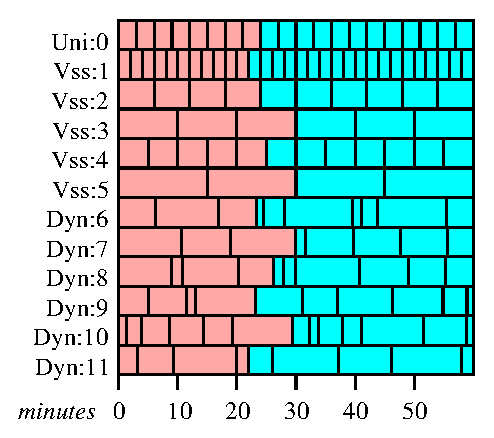
\includegraphics{Figure1}
  \caption{Time scheduling strategies.  Red boxes represent time steps that
    have already passed, blue boxes represents scheduled time steps
    that have not yet been run. ``Uni:''  and ``Vss:'' sub\-models are
    members of a uniform or variable speed splitting
    sub\-models and require uniform time steps, and ``Dyn:'' sub\-models
    have adaptive time steps.}
\end{center}
\end{figure}
A better approach is the technique of variable speed splitting, such
as in~\cite{walters2004fisheries} and many others. (Figure~\ref{times}) This approach allows models to step through time in
different intervals by dividing the largest interval required into
smaller steps that are more appropriate for the sub\-models with
naturally shorter time scales. While models with uniform time steps are
a trivial example of this approach, variable speed splitting is almost
as simple and much more efficient.  This technique can keep the
subjective times of a set of agents moderately consistent, but ad hoc
stepping changes would still seem to be awkward or difficult.

Both of these strategies may be subject to artifacts arising from the
sequence in which agents are given their time step.  The general class
of model errors of the sort described in~\cite{chivers2009generalised}
arise as a consequence of structure of the processing across the set
of agents in a simulation. \IB\ models which process agents
species-by-species will be particularly vulnerable to these sorts of
artifacts, since there will be an implicit advantage or disadvantage
to being early in the list.  Similarly, advantage or disadvantage can
arise when there is a change in rep\-re\-sen\-ta\-tion, perhaps from an
\SD\ sub\-model to an \IB\ sub\-model; a shorter time step in this
situation may introduce a great many small time steps which agents may
exploit.  This kind of problem can be overcome by introducing a
randomizing process within each time step. Early versions of the
variable speed splitting model in~\cite{lyne1994pmez5} suffered from
predator-prey artifacts arising from a na\"{\i}ve introduction of
predators and prey into the list of agents, and such randomizing was
introduced to minimize the effects. In situations where the time steps
of the interacting agents differ, implementing a randomization
strategy may require a significant increase in the complexity of the
system to accommodate irregular stepping through the lists of
agents, or a significant change in the basic structure of the model.

\cite{gray2006nws} and~\cite{fulton2009crossingscales} describe models that have a well %
developed approach to coordinating agents using adaptive time
steps. In these models agents may set their own time steps to
intervals that are suitable for their current activity or role. This
strategy can readily incorporate sub\-models with uniform time steps, or
collections that employ a variable speed splitting strategy. When
agents interact, they either explicitly become synchronous before
interaction occurs by setting their time steps appropriately and
waiting, or they implicitly acknowledge that there is a temporal
mismatch. (Figure~\ref{times})

While some agents should be given execution priority (such as an agent
which models ocean currents), most agents will have their execution
order within a time step randomized, effectively preventing a large
class of execution order dependent artifacts.  The associated overhead
in the most recent work,~\cite{gray2006nws,gray2012adaptive}, is marginally higher
than one would expect from single-stepping or variable speed stepping
systems, but the advantages arising from the ability to ensure
synchrony and change time steps in response to en\-vi\-ron\-men\-tal stimulus
outweigh the small computational overhead.  This last approach seems
likely to be the most appropriate for a general hybrid model that
supports swapping models.

General adaptive hybrid models must have a mechanism for scheduling
each agent's execution which keeps the cohort of agents roughly
synchronous, and it should able to handle changes in an agent's time
step when the agent changes its rep\-re\-sen\-ta\-tion; where possible, agents
should also be designed so that they may run at other time steps as
well as their own preferred time step so they can become synchronous
and interact at the appropriate temporal scale with other agents.

%-- MONITOR structure

\subsection{Systematically adjusting the model con\-fig\-ur\-a\-tion}
%----> Infrastructure, introduce monitor, guff about what should be in a monitor <----

A model's con\-fig\-ur\-a\-tion should only change when there is an overall
benefit in the efficiency or fidelity of the system.  A
straightforward way of determining this is to have a monitoring
routine that runs periodically, polling the agents, and ranking likely
con\-fig\-ur\-a\-tions according to their relative benefit or cost.  This
means that each sub\-model would need a way to provide, to the monitor,
a measure of its current suitability, and to indicate what it needs
from other niches. 


%---- Algorithm MonAlg
\begin{algorithm}\label{MonAlg}
  \caption{Basic processing pass for the monitor}
  \begin{algorithmic}
    \ForAll{niches}
    \ForAll{sub\-models in the niche}
    \ForAll{agents in the sub\-model}
    \State generate agent state vector
    \State generate the sub\-model state vector
    \State \qquad note extrinsic requirements
    \EndFor
    \EndFor
    \State
    \State generate niche state vector
    \EndFor
    \State
    \State Run niche-level assessment
    \State Flag any whole of model issues
    \ForAll{candidate con\-fig\-ur\-a\-tions}
    \State Deprecate untenable con\-fig\-ur\-a\-tion
    \State Adjust for unavoidable extrinsic
    \State $\qquad$ requirements
    \EndFor
    \State
    \State Select best indicated con\-fig\-ur\-a\-tion
  \end{algorithmic}
\end{algorithm} The last step in Algorithm~\ref{MonAlg} is deliberately vague. 

Algorithm~\ref{MonAlg} illustrates a possible
assessment pass for a monitor, though how appropriate it may be is an
open question. Configuration ranking for the example model will be
cast in terms of evaluating an objective function based on elements of
the vector space of tree elements described in the \appendixname.

A monitor may have large number of potential candidate con\-fig\-ur\-a\-tions,
but we would like to keep the actual number quite low. The example
model described below has a global domain associated with a particular
rep\-re\-sen\-ta\-tion, along with local domains (subregions of the global
domain) which are associated with finer scale rep\-re\-sen\-ta\-tions of the
modeled entities. The set of potential candidate trees could be quite
large; in practice we reduce the number by casting the candidate trees
in a more general way -- including trees representing particularly
good rep\-re\-sen\-ta\-tions and particularly poor rep\-re\-sen\-ta\-tions: the first
to steer the con\-fig\-ur\-a\-tion toward good choices, and the second to
drive it away from poor choices. We can use the hierarchical
organisation (whole-model, niche, sub\-model, agent) to help limit our
search space, as well as the geographic context of the agents (whole-domain, local
cell, immediate-locus).

The sets of candidate trees which are associated with particular
con\-fig\-ur\-a\-tions will need to be crafted carefully as a part of the
model design. These trees reflect the modelers understanding of the
strengths and weaknesses of each of the sub\-models (or sets of
different sub\-models) which may be employed.

Exactly how a monitoring routine is integrated into the model
framework is a subjective choice best left to the team implementing
the models, but one very attractive option is to implement the monitor
as an agent in the system. This would allow the monitor to assess its
own performance and the needs of other agents with respect to its own
suitability with the option of swapping itself our for a montitor
which implements some alternative strategy. 


%-- The example model
%--- Algorithmic description of the model
\typeout{Chapter~3: The example model}
\section{The example model}

The purpose of the example model described below, is to provide a
context for a discussion of the dynamics associated with a
hypothetical simulation using this model.  The ends of the
spectrum between \SD\ models and \IB\ models are represented, and the
environment is unrealistically simple in order to keep us from being
swamped by detail. 

\begin{figure}\label{domain}
\begin{center}
  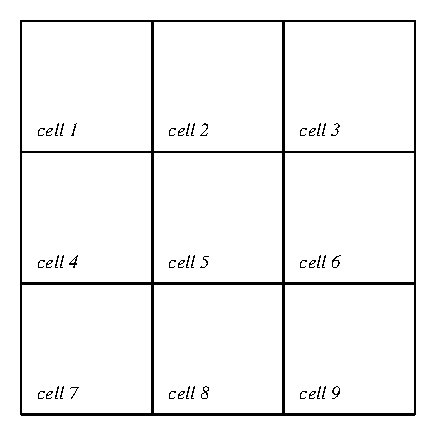
\includegraphics{Figure2}
  \caption{The model domain is divided into nine cells. An \SD\ agent
    is associated with each of these cells and with the domain as a
    whole. Any \IB\ agents which are created during the simulation
    will be associated with one cell at any given time.}
\end{center}
\end{figure}


%----> Describes phys domain, niches, food chain <----
The model consists of a spatially explicit environment that is
partitioned into nine cells (Figure~\ref{domain}). The biotic elements
consist of plants, fruit, seeds, herbivores, and carnivores.  The
herbivores feed on the plants and their fruit; and carnivores prey
upon juvenile herbivores.  The plants and herbivores are
interdependent: fruit is the sole diet for juvenile herbivores and the
plants need juvenile herbivores to make the seeds viable by eating the
fruit.

%----> Introduces rep\-re\-sen\-ta\-tions of entities <----
The rep\-re\-sen\-ta\-tions are equation-based \SD\ models of the interactions
between the plants and animals and \IB\ models for plants and
animals. The \SD\ sub\-models model the biomass with respect
to size, for plants and animals, or simply numeric quantities for
fruit and seeds, and they can operate at either the global or
cell-sized scale. Modeling biomass in this way makes it possible to
minimize the loss of fidelity incurred by swapping from \IB\ agents to
\SD\ agents and visa-versa, since we preserve more of the essential
nature of the populations. A more detailed description of the
\SD\ agents is presented in the \SuppMaterial.

%----- Fruit and seeds

\subsection*{Fruit and seeds}
%------> Describes fruit and seeds <------
Fruit and seeds are treated somewhat differently to the rest of the
niches. They exist principally as numbers of entities that are updated
as a result of the activities of other, more explicit \SD\ or
\IB\ models.  There are explicit routines that deal with uniquely
``fruit'' and ``seed'' processing to handle spoilage and germination,
respectively.

For fruit and seeds we have the following relationships
\begin{equation*}
   d\N{F}(t) = \mathit{Production} - \mathit{Spoilage} - \mathit{FruitEaten}
\end{equation*}
and
\begin{align*}
  d\N{S}(t) = s &* \mathit{FruitEaten} \\
  &- \Biggl(1 - \frac{\N{P}(t)}{\K{P}}\Biggr)\mathit{Germ}.
\end{align*}
where $\N{P}(t)$ is the biomass of plants at time $t$, and $\K{P}$ is
the carrying capacity of the pertinent domain (either global or
cell-based).
%------ fruitalg
\begin{algorithm}\label{fruitalg}
  \caption{Basic processing pass for fruit}
  \begin{algorithmic}
    \State $\N{F} \gets \N{F} - (\mathit{Spoilage}_{\mt{F}} \cdot \N{F})$
  \end{algorithmic}
\end{algorithm}
%----- ...text continues
The processing for fruit is quite simple and consists only of
applying ``spoilage''; no reference to other agents in
the system is required, and only the number of fruit is adjusted as a
result (Algorithm~\ref{fruitalg}).
%------ seedalg
\begin{algorithm}\label{seedalg}
  \caption{Basic processing pass for seeds}
  \begin{algorithmic}
    \State $\mathit{NewTreeCount} \gets \mathit{Germination} \cdot  \mathit{SeedCount}$
    \State $\mathit{SeedCount} \gets \mathit{SeedCount} -  (\mathit{NewTreeCount} $
    \State $\qquad + \mathit{Spoilage}_{\mt{S}} \cdot \mathit{SeedCount})$
    \State generate $NewTreeCount$ new plant agents and introduce them into the system
  \end{algorithmic}
\end{algorithm}
%----- ...text continues
Seed models will adjust their ``seed count'' as well as the biomass
distribution for plants in their time step, according to the level of
germination. Germination is probabilistic as is the size of the plant
a germinated seed becomes in its pass, though the distribution of
possibly sizes is quite restrained (Algorithm~\ref{seedalg}).

%---- SD rep\-re\-sen\-ta\-tions
\subsection*{\SD\ rep\-re\-sen\-ta\-tions}

%------> desciption of animal biomass x size rep. in SD models <------
Each of the niches has an integral equation expressing the change in
biomass for a given size; an animal's equation is of the
form\footnote{See the \SuppMaterial\ for a more detailed set of
  equations.}
\begin{align*}
  d\N{A}(t,x) = & \growthnstarve + \reproduction \\
  & - \predationmort -\naturalmort.
\end{align*}

%------> no migration in SD animal models <------
We do not include migration terms in the \SD\ models, since that will
be addressed by the \IB\ forms. The assumption is that the
\SD\ rep\-re\-sen\-ta\-tion is most appropriate when population levels are
moderately high, and there is adequate food; under these conditions,
we will assume that the net migration associated with a domain will be
close to zero.

%----- Plants 
%------> desciption of animal biomass x size rep. in SD models <------
Plants are represented by similar equations, namely
\begin{align*}
d\N{P}(t,x) = &\Biggl(1 - \frac{\N{P}(t)}{\K{P}}\Biggr)[\growth + \germination] \\- \
& \predationmort - \naturalmort
\end{align*}
where $\N{P}(t,x)$ is the biomass of plants of size $x$ at time $t$.


%------> important state variables for SD models <------
The important state variables for the \SD\ are, for each domain, the
biomass-by-size distributions for plants, herbivores and carnivores, and the
raw numbers of fruit and viable seeds. 

%------ SDalg
\begin{algorithm}\label{sdalg}
  %% if we swap the order of the caption and label, we get the section number
  %% rather than the algorithm number!
  \caption{Basic processing pass for the \SD\ models}
\begin{algorithmic}
  \ForAll{agents in this domain}
    \State{Incorporate quantities that are }
    \State{$\qquad$ controlled in \emph{other} agents}
    \State{Run Runge-Kutta4}
    \State{Update only quantities that are}
    \State{$\qquad$ controlled by \emph{this} agent}
  \EndFor
\end{algorithmic}   
\end{algorithm}

%----- ...text continues

%------> Processing of SD models, justification of non-controlled niches <------
The system of equations described in the \SuppMaterial\ is evaluated
using a fourth order Runge-Kutta algorithm; the numbers of fruit and
seeds, and both the global and cell-based biomass distributions for
plants and animals are updated at the end of the calculation. The
model will adjust the values in the global and cell-based models to
allow data from models running with better resolution (usually more
localized models) (Algorithm {\ref{sdalg}}) to take precedence.

%------> We haven't nailed parameters down, because. <------
Most of the important parameters and many of the functions associated
with the life history of the modeled entities are not specified. This
way we may consider possible trajectories without being tied to a
particular conception or parameterization of the system.


%---- IB rep\-re\-sen\-ta\-tions
\subsection*{\IB\ rep\-re\-sen\-ta\-tions}
%------> introduction of the IB rep, follows Gray2012adaptive <------
Individual-based rep\-re\-sen\-ta\-tions for plants, herbivores and carnivores
follow the pattern in~\cite{little2006nws}; fruit and seeds are only
modeled in the \SD\ rep\-re\-sen\-ta\-tion, though their numbers are modified
by the activities of the herbivores irrespective of how those
herbivores are represented. 

\subsection{\IB\ Plants}\label{plantch3}

%------> Basic  plant state and dynamics <------
Plants maintain a reference to their cell, their location, a mass and
a peak mass.  If a plant's mass drops below a certain proportion
($\ttt{P}_{M\Omega}$) of its peak mass, it dies --- this provides a
means for the herbivores to drive the plant population to local
extinction. 

%------> sigmoidal growth rate <------
We will suppose that plants grow according to a sigmoidal function with
some reasonable asymptote and intermediate sharpness; fruiting
occurs probabilistically as in the \SD\ represen\-tation.

%------ plantalg
\begin{algorithm}\label{plantalg}
  \caption{Basic processing pass for plants}
  \begin{algorithmic}
    \If {$(\mass \ge \Mtt{P}_{\mature}) \land (\ttt{P}_{\fruits} \ge \Urnd)$}
    \State $\AddFruit{\ttt{P}_\rho}{\mass^{\frac{2}{3}}}$
    \EndIf
    \If {$(\mass\le\Mtt{P_{M\Omega}}\,\peakmass)\lor(\imort{P}<\Urnd)$}
    \State \Die
    \Else
    \State $\mass \gets \Gamma_{\mt{P}}(\delta t, \mass)$
    \If {$\mass > \peakmass$}
    \State $\peakmass \gets \mass$
    \EndIf
    \EndIf
  \end{algorithmic}
\end{algorithm}

%------> Describe parameters/variables <------

The plant agent goes through the steps in Algorithm {\ref{plantalg}} in each
of its time steps. In the algorithm, $\Gamma_{\mt{P}}(\delta t, mass)$ is an
analogue of the probability of a plant growing from one size to another from
the \SD\ rep\-re\-sen\-ta\-tion, $\ttt{P}_{\mature}$ is the parameter that indicates
the mass a plant must be before it fruits, $\ttt{P}_{\fruits}$ is the
probability of a mature plant fruiting, and $\ttt{P}_\rho$ is the amount of
fruit relative to the fruiting area. The routine \textsc{AddFruit} updates the
models representing fruit in the domain.

\subsection{\IB\ Animals}

%------> Basic  plant state and dynamics <------
Like the plants, animals maintain a reference to their cell, their
location, and a mass. They also maintain several variables that are
associated with foraging or predation, namely the amount of time until
they need to eat ($\satedtime$), and the amount of time they have been
hungry ($\hungertime$).

Animals will grow while they do not need to eat and will only forage
when they are hungry.  Reproduction happens in a purely probabilistic
way once the animal is large enough, and the young are not cared for
by the parents.

Animal movement is constrained so that they will tend to stay within
their nominated home cell, only migrating (changing their home cell to
an adjacent cell) when food becomes scarce or if the population
exceeds some nominated value and causes crowding.

%------> Growth, starvation and differences w.r.t. SD model <------
The analogues of the mechanisms for growth and starvation in the
\SD\ rep\-re\-sen\-ta\-tion are quite different to those of the \IB\ version.
In the \SD\ models, starvation and growth occur as a result of the
relative population levels of the consumer and the consumed rather
than the local availability of food.

%------> Animals are all the same, really, just initial setup and prey differences <------
There are no real programmatic differences between the
\IB\ rep\-re\-sen\-ta\-tions of herbivores and carnivores; their differences
lie in their choices of food and the way their ``time-to-eat''
variable is initially managed. In\-di\-vidu\-al-based, new-born carnivores
begin with a long time till they need to eat. This reflects a reliance
on some unmodeled foodstuff until they are large enough to prey on
the juvenile herbivores.  In contrast, the juvenile herbivores must
begin eating fruit immediately, and only switch to foraging on plants
when they are larger (but before they can reproduce). For both
species, if the amount of time they have been hungry exceeds a
particular value, $H_\Omega$ or $C_\Omega$, the in\-di\-vidu\-al dies.

%------ animalalg
\begin{algorithm}\label{animalalg}
  \caption{Basic processing pass for herbivores and carnivores}
  \begin{algorithmic}
  \If {$(\imort{A} > \Urnd) \lor (\hungertime \ge \ttt{A}_\Omega)$}
  \State \Die
  \EndIf
  \State {$\preylist \gets \PreyPresent{A}{\location}{\mass}$}
  \If {$\satedtime \ge 0$}
  \State {$\mass \gets \mass + \Growth{A}{mass}{\delta t}$}
  \ElsIf {$(\hungertime \ge 0)\land(\lcount{\preylist} > 0)$}
  \State {$\satedtime \gets \Eat{\preylist}{\ttt{A}_{EatLimit}}{mass}$}
  \State {$\hungertime \gets 0$}
  \State {$\foragecount \gets 0$}
  \ElsIf {$((\hungertime \ge 0) \land len(\preylist) = 0)$}
  \State {\textsc{Forage}}
  \State {$\foragecount \gets \foragecount + 1$}
  \ElsIf {$(\hungertime \ge \ttt{A}_{moveT}) \lor \LocallyCrowded{A}$}
  \State {$\Migrate{A}{\location}$}
  \Else
  \If {$(mass \ge \ttt{A}_{RepSize}) \land (\ttt{A}_{RepP} \ge \Urnd)$}
  $\Reproduce{A}{\location}$
  \EndIf
  \EndIf
\end{algorithmic}
\end{algorithm}
%----- ...text continues

%------> effect of different parameters i.t.o. behavior <------
So, if we take \ttt{A} to represent either carnivores (\ttt{C}) or
herbivores (\ttt{H}) below, then the processing pass for an animal is
shown in Algorithm~\ref{animalalg}, where $\ttt{A}_{moveT}$ is the
amount of time an animal can be hungry before it migrates,
$\ttt{A}_\Omega$ is the amount of time it takes for the animal to
starve, $\ttt{A}_{EatLimit}$ is the most the animal can eat as a
proportion of its mass, $\ttt{A}_{RepSize}$ is the minimum size an
animal may breed at and $\ttt{A}_{RepP}$ is the probability of
reproducing. The routines $\mathsc{PreyPresent}_{\Mtt{H}}$ and
$\mathsc{Eat}_{\Mtt{H}}$ have different cases for juvenile and adult
herbivores, since juveniles prey upon fruit, and the seeds from the
fruit they eat need to be accounted for in the appropriate places. There is
a similar issue with juvenile carnivores. Their \emph{preylist} will
always be set to a value that indicates that they may eat as much as
they like, and the corresponding call to $\mathsc{Eat}_{\Mtt{C}}$ will
handle this value appropriately.


%--- MONITOR: Model dynamics in the example
\subsection{The monitor and model dynamics}
%-------> commands <--------
%% {repset}{sn}
\newcommand{\cst}[1]{\node{\bar{\check{\tau}}}^\Sigma_{#1}} % candidate tree 
                                                       % for config
\newcommand{\domt}[1]{\node{\check{\tau}}^\Sigma_{#1}} % candidate
                                                     % tree for a domain



%% {t}
%% {id} {t}
%% {rep} {id} {t}
%% {rep} {t}
\newcommand{\stmA}[1]{\node{\tau}^\Sigma_{#1}} % the aggregate whole model status tree at $t$
\newcommand{\stsdA}[2]{\node{\tau}^\Sigma_{SD(#1),#2}} % the aggregate cell status tree 
\newcommand{\stibA}[2]{\node{\tau}^\Sigma_{IB(#1),#2}} % the aggregate
                                                     % cell status
                                                     % tree for types
                                                     % of  individuals
%\newcommand{\nstaA}[3]{\node{\tau^\Sigma}_{(#2),#3}\vert_{#1}} % niche status tree
\newcommand{\stm}[1]{\node{\tau}_{#1}} % the whole model status tree 
\newcommand{\sta}[3]{\node{\tau}_{\ms{#1}(#2),#3}} % generic st tree
\newcommand{\stsd}[2]{\sta{SD}{#1}{#2}} % SD st tree
\newcommand{\stib}[2]{\sta{IB}{#1}{#2}} % IB  st tree
\newcommand{\staR}[3]{\node{\tau}_{\ms{#1}(#2),#3}} % generic st tree
\newcommand{\nstaR}[2]{\node{\tau}_{#1,#2}} % niche status tree at t
\newcommand{\nsta}[3]{\node{\tau}_{#1(#2),#3}} % niche status tree
\newcommand{\asta}[3]{\node{\hat{\tau}}_{\ms{#1}(#2),#3}} % alternate 

\newcommand{\stbr}[2]{\child({#1},\mc{#2})}

\newcommand{\gtentry}[4]{{#1} & {#2} & {#3} & {#4}\cr}
%\AsdGtentry{t}{txt}
\newcommand{\AsdGtentry}[2]{{#1} & \stmA{#1} & global \SD & global state in aggregate #2\cr}
%\AsdGtentry{t}{cellnum}{txt}
\newcommand{\AsdLtentry}[3]{{#1} & \stsdA{#2}{#1} & \SD: cell #2 \SD &  characterizes cell #2 in aggregate #3\cr}
%\sdGtentry{t}{txt}
\newcommand{\sdGtentry}[2]{{#1} & \stm{#1} & global \SD & global state #2\cr}
%\sdLtentry{t}{cellnum}{txt}
\newcommand{\sdLtentry}[3]{{#1} & \stsd{#2}{#1} & \SD: cell #2 \SD & characterizes cell #2 #3\cr}
%\ibtentry{t}{id}{rep}{txt}
\newcommand{\ibtentry}[4]{{#1} & \stib{#1}{#2} & \IB: #3 & {#4}\cr}


%------> table of items prompting changes <------
The following may be typical of the types of situations that could or
should cause changes in the con\-fig\-ur\-a\-tion:
\begin{itemize}
  \item \emph{Low population} -- If, in an \SD\ representa\-tion,
    the number of in\-di\-vidu\-als filling a niche (either explicitly taken
    from a distribution, or estimated using a mean and a biomass)
    drops below a nominated value, then the biomass in that niche
    should be converted to \IB\ agents representing those
    in\-di\-vidu\-als. This type of change is motivated by the observation
    that at low population levels the assumption that we can treat the
    population as having uniform access to resources (or be uniformly
    available to predators) breaks down;

  \item \emph{High population} -- If a niche in a cell is
    represented by \IB\ agents and the number of in\-di\-vidu\-als exceeds a
    (higher) nominated value, the biomass those agents represent
    should be subsumed by the distribution in the local
    \SD\ submodel. The change in rep\-re\-sen\-ta\-tion is attractive here for
    two reasons: an equation-based rep\-re\-sen\-ta\-tion will be much faster,
    and \SD\ submodels are arguably simpler to calibrate;

  \item \emph{Starvation risk} -- If the mean amount of time an
    animal in a cell spends \emph{hungry} in a cell exceeds half of
    $\ttt{A}_\omega$ (or some other nominated time), the prey biomass
    must convert to \IB\ agents if it isn't already so (bearing in
    mind that this isn't pertinent for fruit). This mean is calculated
    by averaging the means of each animal in the cell. If this is
    triggered, it indicates that the biomass of the prey species is
    sparse enough that homogeneity assumption is unlikely to hold;

  \item \emph{Relative biomass} -- If the biomass available for
    predation is represented in a local \SD\ agent and its density
    drops below some proportion of the minimum required to support the
    predators in the domain, the prey species should convert its
    biomass into \IB\ agents and, if the predator is represented by a
    \SD\ agent, it should also convert to an \IB\ form. If the
    biomasses are such that the effective predation rate is
    unsustainable, the mixing assumption is unlikely to hold.
\end{itemize}

%------> description of the items in the change table <------
The pertinent data for conditions will be periodically reported to the
monitor through a set of status trees. The trees are able to represent
single entities, nested entities and aggregates equally well, and can
preserve structural information which may also be used in the
comparison of these trees.  One of the basic elements we can easily
incorporate into a sub\-model's status tree is the agent's own
assessment of its competence relative to its state-vector and its
local conditions. This measure of ``self-confidence'' can probably be
maintained at little computational cost for most agents, and may be
the most significant component in a monitor's assessment. The
\emph{high} and \emph{low} population level conditions can clearly be
determined by the agent in question; it can set its level of
self-confidence upward or downward as appropriate. \emph{Starvation}
can also be encoded in the relevant node of an agent's status tree,
but since starvation alone may not indicate a problem with the way the
entity is represented, it probably wouldn't reduce the value for its
confidence.

A starvation trigger may usually arise as a natural consequence of the
population dynamics, but it may also occur when there is a mismatch in
rep\-re\-sen\-ta\-tions which has not been adequately addressed in the design
stage.  The final condition based on the relative biomasses is one
which properly lies in the realm of the monitor -- it would be quite
inefficient for each of the candidate animals to be querying their
prey for available biomass, summing the result, and then noting the
need for change.

%------> status tree types <------

The monitor will primarily use the confidence values associated with
agents and their niches, and the distance from trees which describe
the state of the model or its set of submodels to trees which describe
``known good'' con\-fig\-ur\-a\-tions. With data obtained directly from the
agents in the system and from alternative rep\-re\-sen\-ta\-tions it generates
status trees,
\begin{itemize}
\item{\qquad} $\cst{sn}$, is a candidate status tree tied to a
  specific  con\-fig\-ur\-a\-tion. The serial number, $sn$, ties it to a
  con\-fig\-ur\-a\-tion with that serial number,
\item{\qquad} $\domt{d}$, is a candidate tree which represents the
  current state of a domain,
\item[\qquad] $\stmA{t}$, an aggregate tree for the whole domain at
  time $t$,
\item[\qquad] $\stsdA{n}{t}$, aggregate trees for each cell, $n \in \{1,\ldots, 9\}$,
\item[\qquad] $\sta{R}{i}{t}$, specific status trees for each agent,
\item[\qquad] $\nstaR{R}{t}$, specific status trees for a 
  rep\-re\-sen\-ta\-tion $R$ for each rep\-re\-sen\-ta\-tion associated with a niche,
%\item[\qquad] $\nsta{R}{i}{t}$, specific status trees for 
%  rep\-re\-sen\-ta\-tion, $R$, suitable for modeling things like agent $i$
\item[\qquad] \qquad and
\item[\qquad] $\asta{R}{i}{t}$, candidate trees for all possible
  rep\-re\-sen\-ta\-tions of each agent $i$,
\end{itemize}
at the beginning of each of its steps. The model may have a mix of
\SD\ and \IB\ rep\-re\-sen\-ta\-tions, and some of the trees will have to
incorporate data from many agents ($\stmA{t}$, any of the
$\asta{R}{i}{t}$, and $\nstaR{R}{t}$, for example). A candidate tree is
a status tree which represents an alternative sub\-model in a niche, and
candidate trees are generated for specific agents and for each niche. When the
monitor begins to generate status or candidate trees for a given
agent, it first looks to see if it has generated an appropriate tree
already.  If it finds one, it incorporates or adjusts the tree
appropriately; perhaps by incorporating the agent's biomass  and size
into the tree's data.  We will also denote the con\-fig\-ur\-a\-tion of a
domain (global or local) with $\domt{c}$ where $c$ identifies the
domain in question.

The monitor assesses the trees by calculating aggregate values of
particular attributes, comparing the trees' divergences from allegedly
ideal con\-fig\-ur\-a\-tions, and by looking how uniform groups are -- groups
of in\-di\-vidu\-als that are all very similar are good candidates for
simpler rep\-re\-sen\-ta\-tions. 

We can calculate the average confidence value from any of these trees
by evaluating \[
\frac{\nabs{\nmask(\node{\tau},
    \mc{confidence},0)}}{\supp(\nmask(\node{\tau},
  \mc{confidence},0))},
\]
for example. The trees and functions to manipulate them are described
in the \appendixname.



\begin{figure}\label{timeline}
\begin{center}
  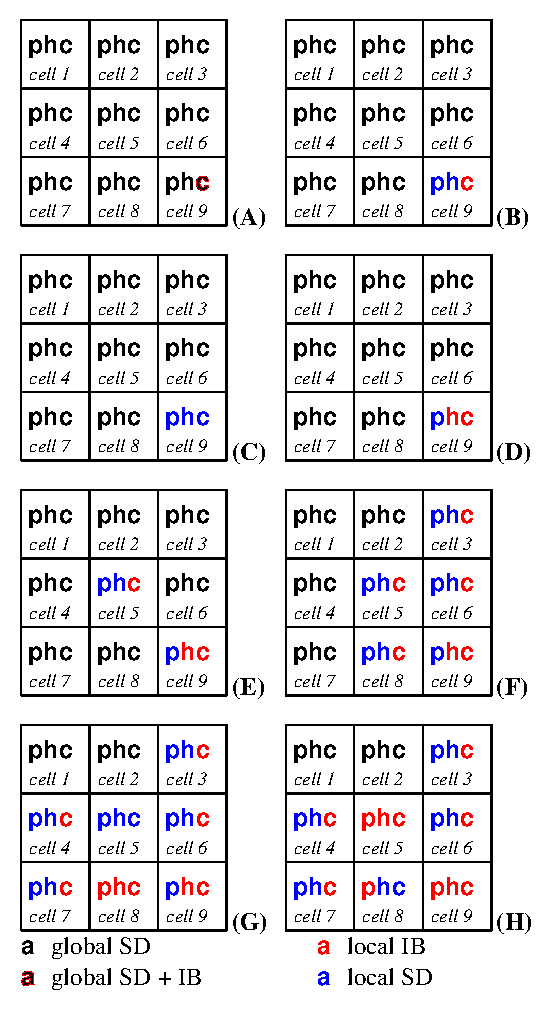
\includegraphics{Figure3}
  \caption{The color of the \textbsf{p},\textbsf{h} and \textbsf{c}
    indicate an agent's current rep\-re\-sen\-ta\-tion within a cell
    at various points in the description of a simulation.  In each, a
    black symbol indicates that the biomass of plants (\textbsf{p}), herbivores
    (\textbsf{h}) or carnivores (\textbsf{c}) is modeled with the global \SD\ agent, a
    blue symbol indicates that the biomass is modeled with a cell's
    \SD\ agent, and red indicates that an \IB\ model is being
    used. Symbols composed of two colors indicate that more than one
    rep\-re\-sen\-ta\-tion is currently controlling portions of the
    relevant biomass.}
\end{center}
\end{figure}

%------> walking through the  <------
Now let us consider what a simulation might look
like. Figure~\ref{timeline}
provides an overview of the con\-fig\-ur\-a\-tion of the system
as our hypothetical simulation runs. The model begins with eleven
agents (not counting the monitor). The monitor runs its first step
generating the status trees: $\stmA{0}$, which characterizes the model
in aggregate, $\stsdA{0}{0},\ldots,\stsdA{9}{0}$, which record the
aggregate state of the ten \SD\ submodels, the aggregate status tree for
the \IB\ agent, $\stibA{0}[9]$, status trees for the \SD\ submodels:
$\stsd{0}{0}$--$\stsd{10}{0}$, the status tree for the lone carnivore,
$\sta{\IB}{11}{0}$, followed by the trees which represent alternative
agents: $\asta{\SD}{0}{0}$--$\asta{\SD}{10}{0}$ and
$\asta{\IB}{11}{0}$.  As mentioned earlier, there is only the single
tree for agent 11 (the carnivore) since its alternative rep\-re\-sen\-ta\-tion
is embodied in $\asta{\SD}{10}{0}$. During the simulation a simulated
fire will occur.

The first steps which must be taken before ranking of potential
configur\-ations is to find the sets of candidate trees which best
approximate the current con\-fig\-ur\-a\-tion at both the global and
cell levels. We do this by calculating a similarity index or a
distance which indicates how close each of the candidate trees are to
the configur\-ation of each of the domains. There are many ways we
could do this: for an index which only considers structural similarity
we might use something like the simple function
\begin{equation*}
  \ssim(\node{c},\node{\tau_d}) =
  \frac{\overlap(\node{c},\node{\tau_d})}{\max(\Tcard{c},\Tcard{\tau_d})}, 
\end{equation*}
but for a more comprehensive treatment which factors values which are
incorporated into the candidate and status trees we might apply the
$\deviO{}{}$ or $\dist{}{}$ functions described in the \appendixname. The
$\dist{}{}$ function is a well-defined distance over the vector space of
trees, while the $\deviO{}{}$ function is an index of similarity that
incorporates structural characteristics as well as the numerical
distance between compatible subtrees.  To refine such an analysis we could apply
$\mask$ and $\nmask$ to select only the relevant parts of the
candidate and status trees.

So to assess the con\-fig\-ur\-a\-tion of a domain, we would use our chosen
measure to construct a set of the results of applying an optimisation
function, $opt$, to each of the candidate trees and their similarity
to the current con\-fig\-ur\-a\-tion.  So if $\set{S}$ is the set of all
serial numbers for candidates, $\domt{d}$ is the status tree fo the
current domain, and  is the, we calculate
\begin{equation*}
  \set(C) = \{(\delta(\domt{d},\cst{i}),i): \forall i \in \set{S}\},
\end{equation*}
and this is used to generate
\begin{equation*}
  \set{C}^* = \{(\opt(\cst{i}),c,\cst{i},i): \forall(c,i) \in \set{C}\}
\end{equation*}
where $\delta$ stands for our chosen measure of similarity.

\begin{figure}\label{indices}
\begin{center}
  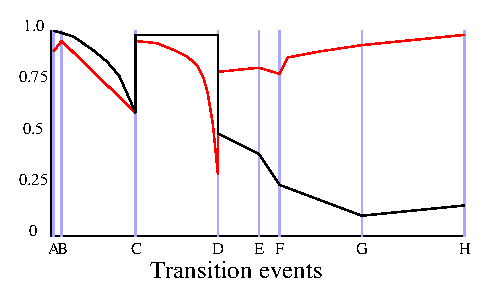
\includegraphics{Figure4}
  \caption{Normalized indexes of execution speed (black) and fidelity (red) the 
    against configuration changes through time associated with Figure~\ref{timeline}}
\end{center}
\end{figure}

The elements in $\set{C}^*$ are then assessed by the monitor, and the
best permissible candidate is selected. If there is only a small
improvement on the current con\-fig\-ur\-a\-tion, $\domt{d}$, the monitor will
leave the con\-fig\-ur\-a\-tion as it is; otherwise, the monitor would then manage
the creation of new agents to replace less optimal rep\-re\-sen\-ta\-tions and
manage the exchange of state data. 




So the early phase of our simulation might begin like so:

\begin{enumerate}
\item %A
Both of the aggregate trees $\stmA{0}$ and $\stsdA{9}{0}$ indicate
that there is an \IB\ agent in their domain and that their
\SD\ rep\-re\-sen\-ta\-tion does not perform well for the indicated
biomass. Both the status and candidate trees for agent 11,
$\staR{11}{0}, \nsta{\IB}{11}{0}$ and $\asta{\IB}{11}{0}$, indicate
that it is confident that it can represent the biomass, and that there
are no immediate unmet requirements from other agents.
Figure~\ref{timeline} (\textbf{A})

\item %B
%-------> Finding a match <--------
The monitor assesses the trees against a prepared set of
con\-fig\-ur\-a\-tions: each of the alternative con\-fig\-ur\-a\-tions (including the
current con\-fig\-ur\-a\-tion) is compared to a set of prepared, ``efficient''
con\-fig\-ur\-a\-tions.  The con\-fig\-ur\-a\-tion of cell 9, $\domt{9}$, notes
global \SD\ rep\-re\-sen\-ta\-tions for plants and herbivores. This
con\-fig\-ur\-a\-tion is ranked lower than the alternative which has an
in\-di\-vidu\-al based model for carnivores and a local \SD\ submodel for the
other entities in the cell.   The monitor makes this change in con\-fig\-ur\-a\-tion,
and informs the global \SD\ agent that it is no longer controlling the
biomasses in cell 9. Figure
\ref{timeline} (\textbf{B})\label{firstconv}

\item\label{cv1}
%-------> Run for a while and convert C to SD <--------
The model may run for some time without any change in con\-fig\-ur\-a\-tion.
Both the herbivores and carnivores breed. The increased execution speed
between \textbf{C} and \textbf{D} in Figure~\ref{indices} is a result
of a change in representation: the number of
carnivores, recorded in $\stsdA{C}{t_4}$, reaches a point that prompts
the monitor to convert them to an \SD\ form.
Figure~\ref{timeline} (\textbf{C})

\item %D
%-------> Run for a while, herbivore population drops  <--------
The biomass of carnivores has increased significantly by the time the
model reaches \textbf{D} in Figure~\ref{indices},
and they are now eating all the young herbivores; as a result the
carnivore population is now prey-limited, and the \emph{Relative
  biomass} condition is triggered.  Both the carnivore and herbivore
populations are converted to \IB\ rep\-resentations. Notice that
dynamics in the fidelity in Figure~\ref{indices} around \textbf{D}
arise from the collapse of the carnivore's prey, followed by the
increase in fidelity after the representation change at \textbf{D}.
Figure~\ref{timeline} (\textbf{D})

\item %E
%-------> + monitor converts cell 5 in fashion analogous to start  <--------
A carnivore, agent 43, has been hungry $(\hungertime \ge
\ttt{A}_{moveT})$ and has migrated to the cell 5
(noted in $\sta{\IB}{43}{t_5}$). As occurred in cell 9 at step~\ref{firstconv}, the monitor
converts plants and herbivores in cell 5 to a local
\SD\ rep\-re\-sen\-ta\-tion, with \IB\ carnivores. Figure~\ref{timeline}
(\textbf{E})

\item %F
%-------> H biomass still too large w.r.t C, but C is hungry #2 %<--------
A lot of activity has occurred in this monitor interval: 
a \emph{Starvation risk} is triggered in cell
9 because too many of the carnivores are hungry (many of the
$\sta{\IB}{n}{t_7}$ trees indicate that the elapsed time without eating is
greater than $\hungertime$). There has been more migration to
cells 5,6 and 8 from cell 9 (more of the $\sta{\IB}{n}{t_7}$ trees
indicate residence in new cells), and a chance migration has introduced a
carnivore into cell 3 from cell 5. Cells 3,6 and 8 are converted to
local \SD\ and \IB\ rep\-re\-sen\-ta\-tions as happened in step
\ref{cv1}. Figure~\ref{timeline} (\textbf{F})

\item %G
%-------> cell 9: C pop crashes <--------
The population of carnivores in cell 9 crashes as a result of
migration and the scarcity of prey, (reported in $\domt{9}$) The
\IB\ juvenile herbivores are patchy and harder to find, so only a few
carnivores are getting enough to eat. There will be many
$\sta{\IB}{n}{t_{10}}$ which indicate hunger or death due to
starvation. The monitor cleans up the dead agents.  There are chance
migrations from cell 5 into cells 4 and 7 (in $\stsdA{4}{0}$ and
$\stsdA{7}{0}$). A fire begins in cell 8, moving through cell 5:
biomass loss in all niches causes all niches to shift to
\IB\ rep\-re\-sen\-ta\-tions. Figure~\ref{timeline} (\textbf{G})

\item %H
%-------> cell 9: Hj begins to appear, but P biomass converts (\#3) <--------
Juvenile herbivores are reappearing in cell 9, but the available plant
biomass (recorded in $\stsd{9}{t_{11}}$) has dropped due to reduced
germination rates, triggering the \emph{Relative biomass} condition in
cell 9 causing the plants to convert to an \IB\ rep\-re\-sen\-ta\-tion.  The
fire in cell 8 has killed all animal biomass in the cell; they
\emph{do not} return to the global \SD\ rep\-re\-sen\-ta\-tion because their
status trees diverge by too much.  Instead, they convert to local
\SD\ rep\-re\-sen\-ta\-tions (which represent zero biomass quite
efficiently). Plants remain as \IB\ agents The fire spreads to cell
5. Figure~\ref{indices} shows a modest increase in execution speed
between \textbf{G} and \textbf{H} due to the population losses
associate with the fire. 
Figure~\ref{timeline} (\textbf{H})

\item[$\bullet$] \ldots the simulation continues
\end{enumerate}


%-- Discussion
\typeout{Chapter~3: Discussion}
\section{Discussion}
%-----> Where do we put the smarts? <-----

Adaptive hybrid models \emph{can} be constructed so that each
submodel is aware of its other rep\-re\-sen\-ta\-tions and is able to change
form as appropriate~\citep{gray2012adaptive}. This approach requires each 
model to have a reasonably close coupling with its alternative
rep\-re\-sen\-ta\-tions, and the burden of instrumenting (and maintaining) the
necessary code quickly becomes untenable in complex models.  Worse, it
removes the possibility of more subtle con\-fig\-ur\-a\-tion management that
can accept poor performance in one part of a system in exchange for
much better performance elsewhere.  It seems that a guiding principle
should be that in an adaptive hybrid model, each rep\-re\-sen\-ta\-tion should
know only as much about the rest of the model as it \emph{must} know,
and no more. The facility for a sub\-model to delve into the workings of
other sub\-models, or the workings of the model as a whole, decreases
the clarity that hybrid modeling makes possible, and opens avenues
for unwanted, unanticipated behavior.

The major argument in favor of closely integrated rep\-re\-sen\-ta\-tions for
sub\-models is that it makes common (or at least similar) state
variables easy to maintain across rep\-re\-sen\-ta\-tions, even in the face of
many rep\-re\-sen\-ta\-tion changes. It is an attractive arguement, but the
long term consequence is an ever growing burden of code maintenance.

Constructing hybrid models isn't significantly more complex than
constructing traditional models. Adaptive hybrid models of the sort
described in this paper will require a more significant investment in
the design of a monitoring routine, and in the crafting of appropriate
sets of candidate con\-fig\-ur\-a\-tions.  The transition dynamics such a
model will exhibit depend on the sets of candidate con\-fig\-ur\-a\-tions, and
it seems likely that a combination of analysis and experimentation may
be the most effective way to develop a set of useful con\-fig\-ur\-a\-tions.
The hybrid models associated with~\cite{lyne1994pmez5, little2006nws,
  fulton2009crossingscales} were built by extending the repertoire of ways of
representing elements of the ecosystem or the anthropic components
rather than wholescale redesign and replacement.

We can imagine an ideal adaptive hybrid model, where any state
information which must be passed on is accompanied by an appropriate,
opaque parcel of code to perform the maintenance. As long as the
monitor knows what information each of these maintenance interfaces
needs, they can be updated each time the monitor interrogates the
agent which has control of the state data.  This is a readily
attainable ideal: many programming languages support first class
functions with closures, and these features are precisely what we need
to address this problem.  \textsl{Scheme, Python, ML, Common Lisp,
  Lua, Haskell}, and \textsl{Scala} all have first order functions
with closures and, hence, the capacity to build model systems with this
capability.

The state vectors and their supporting maintenance procedures can be
treated as data and passed in lists associated with the status
trees. If a monitor decides to swap rep\-re\-sen\-ta\-tions, the accumulated
lists of maintenance functions may be passed on to the new
rep\-re\-sen\-ta\-tion.  A new rep\-re\-sen\-ta\-tion inherits a maintenance list with
variables that are part of its native state, it can claim them as its
own and continue almost as though it had been running the whole
time. In this way, a new rep\-re\-sen\-ta\-tion doesn't need to know anything
about its near kin, only that it must be able to run these black-box
functions that come from other sub\-models, and to pass them on when
required.

It may seem that this concentrates the global domain knowledge in the
monitor, but this is not really the case.  The monitor knows how to
blindly query agents for state data and to the data in maintenance
procedures. The monitor also knows how to recognize and rank
characterizations of the states of the submodels or niches and to use
those data to select a con\-fig\-ur\-a\-tion.

The domain knowledge is encapsulated in the sets of targets the
monitor matches the current con\-fig\-ur\-a\-tion against, and in the
heuristic triggers (such as \emph{Starvation risk}) associated with a
sub\-model or niche.

The essential problems any monitor is likely to deal with are
problems of set selection (recognition, pattern matching\ldots) and
optimisation.  These are common tasks: web searches, voice
recognition, and route planning have become ingrained parts of modern
society. Like route planning, the monitor needs to be able to reassess
the ``optimal'' strategy as an ongoing process.

%----> decision trees,NN,BN,SVM, example uses trees  <----

There are many options to choose from to rank con\-fig\-ur\-a\-tions. A few of
the likely candidates include
\begin{itemize}
  \item using an objective function to evaluate each of the possible
    con\-fig\-ur\-a\-tions,
  \item selecting a con\-fig\-ur\-a\-tion based
    on decision trees,
  \item
    using neural nets to match model states and direct
    us to an appropriate con\-fig\-ur\-a\-tion,
  \item using Bayesian networks to determine the most likely
    candidate,
  \item[and]
  \item using support vector machines to select the
    target/con\-fig\-ur\-a\-tion pairs.
\end{itemize}

In writing this paper, one of the vexing difficulties has been finding
a suitable math\-e\-mat\-i\-cal rep\-re\-sen\-ta\-tion which would allow comparisons
between con\-fig\-ur\-a\-tions, sub\-model states and the states of niches.  We
need proxies that describe models and con\-fig\-ur\-a\-tions of models in a
way that we may readily understand, manipulate and reason about, and
being able to deal with sub\-models which are, in themselves, adaptive
hybrid models, seems to be a naturally desirable trait.  The vector
space of trees described in the \appendixname\ has some nice
properties, and may be directly useful with many of the options above:
it forms a commutative ring (without necessarily having a unit), and
would naturally inherit the body of techniques which only require the
properties of such a ring.

%-- Conclusion
\typeout{Chapter~3: Conclusion}
\section{Conclusion}

There are still some major obstacles to developing a fully fledged
adaptive hybrid model which is generic enough to tackle instances as
varied as marine ecosystem modeling and urban planning. Foremost is a
relative lack of real examples.  The simulation of the hypothetical
model\footnote{The model described in this paper is currently under
  development and will be made freely available when it has been
  completed.}  has tried to expose the character of an adaptive hybrid
model which uses a monitor to manage the con\-fig\-ur\-a\-tion of the system.
There are parts of the description of the example system which are
conspicuous by their absence; this is largely because they lie in
almost wholly uncharted water.  As a modeling community, we need to
develop a wide range of approaches to how a model may assess the
relative merits of a set of con\-fig\-ur\-a\-tions. Many of the mechanisms we
need for adaptive hybrid models already exist, but are found in domain
specific models, and in wholly different domains, such as search
engines and GPS navigation.

Establishing a suitable math\-e\-mat\-i\-cal represen\-tation for model
con\-fig\-ur\-a\-tions which gives us access to well developed techniques for
set selection, pattern recognition and component analysis would seem
to be almost as urgent as adaptive hybrid examples of real systems.


\noindent\emph{Acknowledgments}\linebreak
The authors would like to thank two anonymous reviewers whose comments
have improved the paper immeasurably.  Thanks also go to a patient and
understanding editor at Frontiers, and to Dr Tony Smith, who gave up a
weekend to work a scientifically and grammatically fine toothed comb
through the paper.  The responsibility for any mistakes, awkward
sentences, or places where it just does not make sense now rests
completely with the lead author.


%-  Bibliography

%\bibliography{biblio}
%%\bibliographystyle{frontiersSCNS}
%\bibliographystyle{plain}

%- Appendices

%\appendix


%-- Appendix: Mathematical section

%% The mathematics formats poorly in two column mode.
\onecolumn

\typeout{Chapter~3: \appendixname}
\section{\appendixname}
\subsection{Mathematical definitions}\label{AppTrees}
The trees we use are members of a normed vector space: we can add
them, find out how far apart they are and interpolate between them. In
principle, we can run clustering algorithms to find con\-fig\-ur\-a\-tions
that are similar, and identify when a model has left one cluster and
entered another.

%--- Preliminary definitions

%---- Domain 
\begin{definition}\label{defdomain}
  Let $\mc{S}$ be a set of labels, and let \TFIELD be a field like
  the real or complex numbers. Then we define a node $\node{n}$ as a
  triplet of the form $(\mc{s}, v, \set{E})$, with $v \in \FIELD$,
  $\mc{s} \subset \mc{S}$, and the set $\set{E}$ is a (possibly empty)
  set of nodes of the same form with the restriction that no two nodes
  in $\set{E}$ may have the same label in their first ordinate.  We
  also define the triple $\nulltree = (\emptyset, 0, \emptyset)$,
  which we will call the null tree, and define \TDOM\ to be the union
  of the set of all trees composed of a finite number of these nodes.

  The ordinates of $\node{u} = (\nlabel{u}, \nv{u}, \extn{u})$ in
  \TDOM\ correspond to its \emph{label}, \emph{value}, and
  \emph{extension set}.  An element of $\extn{u}$ will be called an
  \emph{extension}.
\end{definition}


%---- Terms 
In our discussion, it will help to have a few more descriptive terms.

A node with an empty extension set is called a \emph{simple}
node, if this node happens to be a root node, then it is a simple tree.

Two trees, $\node{u}, \node{v} \in \DOM$ are called
  \emph{compatible} if either $\nlabel{u} = \nlabel{v}$ or at least
  one of \tnode{u} and \tnode{v} is \tnulltree.

We define the \emph{depth} of a tree with:
  \begin{align*}
    \depth(\node{u}) = \begin{cases}
      0 & \text{ if } \node{u} = (\emptyset,0,\emptyset) = \nulltree \\
      1 & \text{ if } \node{u} \text{ is a simple node} \\
      1 + \max(\lbrace\depth(\node{v}):\forall \node{v} \in \extn{u}\rbrace) & \text{otherwise.}
    \end{cases}
  \end{align*}

We will also define for \(\node{u} \in \DOM\),
  \begin{align*}
    \trim(\node{u}) = \begin{cases}
      \nulltree & \text{ if } \node{u} = \nulltree \\
      \nulltree & \text{ if } \node{u} \text{ is simple} \\
      (\nlabel{u}, \nv{u}, \lbrace \trim(\node{e}): \\
      \qquad\qquad\forall\node{e}\in\extn{u} \rbrace \setminus \{\nulltree\}) & \text{otherwise.}
    \end{cases}
  \end{align*}

The cardinality of a tree is the number of nodes it
  contains. Specifically, 
  \begin{align*}
    \Tcard{\node{u}} = \begin{cases}
      0 & \text{ if } \node{u} = \nulltree\ \\
      1 + \sum_{\node{e}\in\extn{u}} \Tcard{\node{e}} & \text{otherwise.}
    \end{cases}
  \end{align*}

  Simple nodes are the only nodes that have a cardinality of one, and \tnulltree\ is the only node or tree with a
  cardinality of zero.

The support of a tree is the number of nodes which have a
  non-zero value.
  \begin{align*}
    \supp(\node{u}) = \begin{cases}
      0 + \sum_{\node{e}\in\extn{u}} \supp(\node{e}) & \text{ if } \nv{u} = 0 \\
      1 + \sum_{\node{e}\in\extn{u}} \supp(\node{e}) & \otherwise.
    \end{cases}
  \end{align*}

Related is the fundamental support of a tree, which only counts nodes
with no zero valued nodes in their connection to the root node
  \begin{align*}
    \fund(\node{u}) = \begin{cases}
      0 & \text{ if } \nv{u} = 0 \\
      1 + \sum_{\node{e}\in\extn{u}} \fund(\node{e}) & \otherwise.
    \end{cases}
  \end{align*}
  Clearly the support of a tree, $\supp{\node{u}}$,  must lie in the
  domain $[0,\Tcard{\node{u}}]$ and $\fund{\node{u}} \le \supp(\node{u})$.


The \emph{overlap} between two trees is defined
  \begin{align*}
    \overlap(\node{u},\node{v}) = \begin{cases}
      0 & \text{ if } \node{u} = \nulltree \mor \node{v} = \nulltree \mor \nlabel{u} \neq \nlabel{v} \\
      1 + \displaystyle\sum_{\substack{\node{e}\in\extn{u} \\ \node{f}\in\extn{v}}} \overlap(\node{e},\node{f}) & \text{otherwise}
    \end{cases}
  \end{align*}

  Clearly two trees, \tnode{u} and \tnode{v}, are compatible if and only if \(\overlap(\node{u},\node{v}) \neq 0 \); they will
  be said to \emph{completely overlap} if \(\Tcard{\node{u}} = \Tcard{\node{v}} =
  \overlap(\node{u},\node{v})\).


%--- Scalar multiplication 

We can now define scalar multiplication, and tree addition.
\begin{definition}\label{defscalar*}
  Take $a \in \FIELD$ and $\node{u} \in \DOM$, then
  \begin{equation}
    a\node{u} = \begin{cases}
      %%      \nulltree & \text{if } a = 0 \mor \node{u} = \nulltree \\
      \nulltree & \text{if } \node{u} = \nulltree \\      
      \bigl(\nlabel{u}, a\nv{u}, \{a\node{f}: \node{f} \in \extn{u}\}\setminus\{\nulltree\}\bigr) & \text{otherwise.}
    \end{cases}
  \end{equation}
\end{definition}



%--- Tree addition

\begin{definition}\label{deftree+}
  Let $\node{u}$ and $\node{v}$ be compatible elements of \TDOM.\@Then taking the
  symbol $+$ to be addition in the field \TFIELD, we extend  it to addition in
  \TDOM\ so that for nodes \tnode{u} and \tnode{v},

  \begin{align}
    \node{u}+\node{v}=\begin{cases}
    \nulltree & \text {if } \node{u} = \node{v} = \nulltree \\
    %%!    \nulltree & \text {if } \extn{u} = \extn{v} = \nulltree \mand \nv{u} = \nv{v} = 0 \\
    %% we don't really want to loose the data associated with the labels---zero is a valid number after all 
    \node{u} & \text {if } \node{u} \neq \nulltree \mand  \node{v} = \nulltree \\
    \node{v} & \text {if } \node{u} = \nulltree \mand \node{v} \neq \nulltree  \\
    (\nlabel{u}, \nv{u} + \nv{v}, \emptyset) & \text{if } \extn{u}, \extn{v} = \emptyset \\
    \Bigl(\nlabel{u}, \nv{u} + \nv{v}, \bigl(\{\node{f}+\node{g}:\node{f}\in\extn{u}\mand\node{g}\in\extn{v}\mand\nlabel{f}=\nlabel{g}\} & \\
    \qquad\cup\{\node{f}:\node{f}\in\extn{u}\mand\nlabel{f}\neq\nlabel{g}\forall\node{g}\in\node{v}\} & \\
    \qquad\cup\{\node{g}:\node{g}\in\extn{v}\mand\nlabel{g}\neq\nlabel{f}\forall\node{f}\in\node{u}\}\bigr)\setminus\{\nulltree\}\Bigr)  & \text{otherwise.}
    \end{cases}
  \end{align}
\end{definition}

%--- Tree inner-multiplication

\begin{definition}\label{deftree*}
  Let $\node{u}$ and $\node{v}$ be compatible elements of \TDOM.\@Then 
  we define inner-multiplication between the two nodes
  \begin{equation}
    \node{u}\cdot\node{v} = \bigl(\nlabel{u}, \nv{u} \nv{v}, \{\node{f}\cdot\node{g}: \node{f} \in \extn{u},\node{g} \in \extn{v} \mand \nlabel{f} = \nlabel{g}\}\setminus\{\nulltree\}\bigr)
  \end{equation} 
\end{definition}



%--- Assert vector space, define \nabs{\node{u}}

It can be shown that \TDOM\ with scalar multiplication and tree addition forms a vector space. This
isn't quite enough to give us distances between trees, however, so we define a semi-norm
\begin{definition}\label{defnabs}
  Let \tnode{u} be an element of \TDOM.\@Then we can define a semi-norm over \TDOM
  \begin{align*}
    \nabs{\node{u}} = \begin{cases}
      0 & \text{ if } \node{u} = \nulltree \\
      \abs{\nv{u}} & \text{ if }\extn{u} = \emptyset \\
      \abs{\nv{u}} + \sum_{\node{e}\in\extn{u}}\nabs{\node{e}} & \text{otherwise.}
    \end{cases}
  \end{align*}
\end{definition}


It is clear that $\nabs{\node{u}}$ will always be non-negative, and the only shortcoming is that we
can have a node \tnode{u} with $\nabs{\node{u}} = 0, \mbut \node{u} \neq \nulltree$.  In order to turn
this into a normed vector space we take the set $\nullspace = \{\node{u}: u \in \DOM \mand
  \nabs{\node{u}} = 0\}$ and we construct an equivalence relation on \TDOM\ by the rule $[\node{u}]
\equiv [\node{v}]$ if and only if there exist $\node{z_u}, \node{z_v} \in \nullspace$ such that
$\node{u} + \node{z_u} = \node{v} + \node{z_v}$.  It can be shown that scalar multiplication,
tree addition, \blockcomment{tree multiplication,} and the semi-norm behave appropriately with
respect to the equivalence classes. This means that if we identify
elements of \TDOM\ with their equivalence class, then we can take $\nabs{\node{u}}$ to be a norm and
that it induces a distance function \[\dist(\node{u},\node{v}) = \nabs{\node{u} - \node{v}}.\]

%----- Define mask and nmask

\begin{definition}\label{mask}
  We define the functions $\mask$ and $\nmask$ that set the values
  associated with particular nodes in a tree to $v\in\FIELD$.  Specifically,
  if $\mc{L} \subset \SDOM$, then
  \begin{equation}
    \mask(\node{u},\mc{L},v) = \begin{cases}
     (\nlabel{u}, v, \{\mask(\node{f},\mc{L},v):  \node{f}\in\extn{u}\}) & \text{ if } \nlabel{u} \in \mc{L} \\
      (\nlabel{u}, \nv{u}, \{\mask(\node{f},\mc{L},v): \node{f}\in\extn{u}\}) & \text{otherwise}
    \end{cases}
  \end{equation}
  and
  \begin{equation}
    \nmask(\node{u},\mc{L},v) = \begin{cases}
     (\nlabel{u}, v, \{\nmask(\node{f},\mc{L},v):  \node{f}\in\extn{u}\}) & \text{ if } \nlabel{u} \not\in \mc{L} \\
     (\nlabel{u}, \nv{u}, \{\nmask(\node{f},\mc{L},v): \node{f}\in\extn{u}\}) & \text{otherwise.}
    \end{cases}
  \end{equation}
  $\mask(\node{u},\mc{L},0)$ would return a tree similar to \tnode{u},
  but all its nodes that have labels in $\mc{L}$ would have values of zero.

  We also define several functions which prune or select a child from
  a tree's extension set. This function returns only the part of
  \tnode{u} which overlaps \tnode{p},
  \begin{equation}
    \excise(\node{u},\node{p}) = \begin{cases}
      (\nlabel{u}, \nv{u}, \{\excise(\node{f},\node{g}): \node{f}\in\extn{u} \mand \node{g}\in\node{p} \mand \nlabel{f} = \nlabel{g}\} \setminus \{\nulltree\}) & \text{ if } \nlabel{u} = \mc{L} \\
      \nulltree & \text{ if }  \nlabel{u} \neq \nlabel{p} \\
      (\nlabel{u}, \nv{u}, \emptyset) & \text{otherwise,}
    \end{cases}
  \end{equation}
  and this one either returns an appropriately labelled child from the extension set (a
  branch), or \tnulltree.
  \begin{equation}
    \child(\node{u}, \mc{l}) = \begin{cases}
      \node{f} & \text{ if } \nlabel{f} = \mc{l} \mand \node{f} \in  \extn{u} \\
      \nulltree & \text{otherwise.}
    \end{cases}
  \end{equation}

%%%% This is really wrong: relabel would introduce multiple nodes with
%%%% the same labels into an extn set.
  %%
  %% We also define a relabelling function $\relabel$, where the label of
  %% a node is replace with another, $\mc{l}$, if the nodes label is a member of a
  %% set of labels, $\mc{L}$
  %% \begin{equation}
  %%   \relabel(\node{u},\mc{L},\mc{l}) = \begin{cases}
  %%    (\mc{l}, v, \{\relabel(\node{f},\mc{L},\mc{l}):  \node{f}\in\extn{u}\}) & \text{ if } \nlabel{u} \in \mc{L} \\
  %%     (\nlabel{u}, \nv{u}, \{\relabel(\node{f},\mc{L},\mc{l}): \node{f}\in\extn{u}\}) & \text{otherwise,}

  %%   \end{cases}
  %% \end{equation}


\end{definition}

%--- define deviation

We now finish with a definition of a function, $\deviO{}{}$, that gives us a
measure of the degree of divergence between two trees.
\begin{definition}\label{defdeviation}
  The degree of deviation between two trees, \tnode{u} and \tnode{v} is given  by the expression
  \begin{equation}
    \devi{\node{u}}{\node{v}} = \begin{cases}
      \Tcard{u} + \Tcard{v} - 2\overlap(\node{u},\node{v}) + \nabs{\node{u} - \node{v}}&\text{if }\node{u} \mand \node{v} \text{ are compatible} \\
      \Tcard{u} + \Tcard{v} & \text{ otherwise.}
    \end{cases}
  \end{equation}
  
  The rationale behind this definition is that if trees \tnode{u} and \tnode{v} are identical, then
  $\devi{\node{u}}{\node{v}}$ will be zero. We also want nodes that aren't common to both trees to
  count as differences.
\end{definition}
%%%\end{document}

\typeout{Chapter~3: Epilogue to the paper}
\section{Epilogue to the paper}

The model described in this paper has been used as a template for the
model discussed in \Cfive. The paper attempted to
describe a credible ``toy'' model to provide a setting for the
discussion. Unfortunately, when it came to implementation of the model
the paper described, a few shortcomings came to light and some of the
corresponding algorithms have been altered in the explicit
model to correct them.  The most notable example, and one which
characterises them well, is that adhering to the description
effectively prevented cells which are stripped of living plants from
being recolonised.  As stated, the seeds resulting from the
consumption of fruit were tied to the cell they were eaten in, because
the animals excreted them immediately. The consequence of this was
that there was no way for plants to recolonise empty cells.

This paper extended and generalised the simple state maintenance of
\Ctwo by passing closures rather than a vector
of values and the confident knowledge that the closures embodied the
correct process for update. By using closures, the actual machinery
supporting the update of the state of a previous representation can be
passed and both the mechanism and data made, in some sense, opaque to
all but the representation it is associated with. Enforcing the notion
that the code required for maintaining a state vector of a
representation must be provided \emph{by} that representation means
that all of the code which changes the state of an agent is embodied
within the agent's representation.  This has practical appeal in that
inappropriate modifications to that state data may cause errors that
would be very difficult to isolate.

The trees described in the next chapter are used to characterise the
distribution of agents within the model's spatial domain, and encode
the different representations and numbers of those agents. 
  % Definitions, proofs
% -*- outline-regexp: "%--* ";  -*-
\chapter[A RING-LIKE STRUCTURE OF TREES]{A non-unital ring-like structure of trees}\label{treering}
\section{Introduction}
The project which triggered the development of the structure in this
chapter considered using the modeling of the social dynamics
associated with policies about, and responses to climate change and to
predict the social and economic consequences of development arising
from various scenarios. This was a significant change from previous
representations of ``public'' participants, such as recreational
fishers, tourists, accomodation and other small businesses, which were
modelled in fairly simple ways (\cite{Fulton2011ningaloo,gray2014}).
The specific goal was to be able to incorporate a simulation of the
way public opinion changes in response to policy actions and changes
in the economy and environment.  The starting point for this was a
corpus of responses to a survey on attitudes associated with the topic
of climate change (\cite{boschetti2012}). The data consisted of
(largely) numeric answers to individual questions which could
represented as either distinct items, or as an aggregation of symbolic
elements.  Questions like ``How much do trust the following
individuals or organisations to tell you the truth about changing
climate?'' might be encoded in a symbolic way by aggregating the
symbols \textsf{climate\_change, trust, information\_source, AustPeng}
for the trustworthiness of the \emph{Australian Penguins} as a source
of information. The actual value marked could be encoded as a scalar,
giving us an expression like ``\textsf{4/5 + climate\_change +
  information\_source + trust + AustPeng}''---expressing it in this
way suggested that working with more intricate relationships might be
possible.

While my involvement in the project was shortlived, the problem the
data posed was engaging, and slowly it became evident how the the
mathematical structures I was trying to construct could represent
configurations of models, and that it might be able to incorporate the
interdependencies between models and other information in a very
simple way.  My hope was to be able to construct example
configurations which were reasonable for particular conditions and to
assess how close to ``known-good'' configurations the system was at
any given point.  It also seemed possible that it might allow
strategies which were apble to interpolate between ``good''
configurations making intermediate transitions between configurations
feasible. The natural network of dependencies exhibited by some
components of past models suggested using tree structures to encode
the configuration of a model as a starting point.

The structure described in this chapter is the structure behind the
work in Chapter \ref{adaptiveselection}.  The trees are comprised of
nodes which have a label and a weight (and, of course, children).
Initially, the labels were simply symbols associated with certain
attitudes or semantic data which were taken from a nominated set.
This had the advantages of simplicity and clarity, but their very
simplicity made the multiplicative operator much more complicated. I
realised that much of the machinery associated with labels was really
just a messy version of arithmetic in commutative ring-like structure of
multinomials. I believe that using the field of rational multinomials
may be productive, but this notion has not been seriously explored.
Once labels were identified with multinomials, everything became
clear.

\section{Conventions and preliminary definitions}

Generally, we will use lower case, boldfaced symbols to denote a node
(or tree), and upper case, boldfaced symbols to denote sets ---
particularly sets of nodes.  Other symbols (such as \(x\)) will
typically refer to numbers or \polyrat \polyforms. Elements of a
node, \tnode{u} will be identified using an appropriate subscript,
namely \tnv{u}, for the node's value and \tnlabel{u} for its
label. Initially, the children of a node were thought of as
refinements or children of an attitude, so the children of $\node{u}$
were its children, and \tchild{u} denotes the set of children.  We will
take $\PLY{A}$ to be the \polytypes over the elements of a finite set
of symbols $\set{A}$.  Here $\FIELD$ would usually be some numeric
field such as $\mB{Q, R}$ or $\mB{C}$, for example.

\begin{definition}\label{def-of-dom}
  Given $\set{A}$ and $\PLY{A}$ and an arbitrary field, $\FIELD$, we
  define the set, $\DOMstar$ of finite (acyclic) trees where each node is
  of the form $(\nv{u}, \nlabel{u}, \child{u})$ where the value,
  $\nv{u}$, is a member of $\FIELD$, it's label, $\nlabel{u}$ is
  a member of $\PLY{A}$ and the set of children, $\child{u}$, contains
  leaf nodes with distinct labels.
\end{definition}

Nodes or trees with no children, \(\set{E} = \emptyset\), will be
called \emph{simple nodes, simple trees}, or \emph{leaf nodes}, and
simple nodes which also have scalar multinomials as their labels may
be referred to as \emph{scalar nodes} or \emph{scalar trees}. The
domain of trees, $\DOMstar$, is the collection of only those trees with a
finite number of nodes.  form. We will make use of a special element
in $\DOMstar$, $\zerotree = (0, 0, \emptyset)$, which is an an analogue of
zero that we will call the \emph{zerotree}.

In this work, we will largely be concerned with a subset of
$\DOMstar$, $\DOM$ which consists only of trees whose root nodes have
a label equal to zero. This subdomain obviously includes \tzerotree,
and will be closed under the arithmetic operations we define. The
other


%% \begin{definition}
%% A node, $\node{u}$, is a representative of a recursive, acyclic
%% structure of the form $(v, p, \set{E})$ where we have $v \in \FIELD, p
%% \in \PLY{A}$, and the children, $\set{E}$, contains nodes of the
%% same for, with the caveat that the labels of the elements must be
%% unique within the set. Without necessarily limiting ourselves, we will
%% take $\FIELD$ to be $\REAL$.  Nodes or trees with \(\set{E} =
%% \emptyset\), the empty set, will be called \emph{simple nodes, simple
%%   trees}, or \emph{leaf nodes}, and simple nodes which also have
%% scalar multinomials as their labels may be referred to as \emph{scalar
%%   nodes} or \emph{scalar trees}. The domain of trees, $\DOM$, is the
%% collection of only those trees with a finite number of nodes.
%% form.
%% %%%, with the caveat that we exclude nodes with \omit{scalar multinomials} and
%% %%%non-empty children.
%% We will make use of a special element in $\DOM$, $\zerotree = (0, 0,
%% \emptyset)$, an analogue of zero which we will call the
%% \emph{zerotree}.

%% The set of valid labels is taken to be a commutative ring of
%% multinomials, $\PLY{A}$. In principle, elements of \emph{any}
%% (commutative) ring could serve equally well.
%% \end{definition}

Note that the choice to use elements of the \polytypes for labels is, in a
sense, arbitrary: elements of any commutative ring will serve, though
we will see that if we use a commutative ring, $\DOM$ and the derived
domains are also commutative; here, the \polytypes provide a
simple example which is easily manipulated and printed. 
$\FIELD$ is taken to be $\mathbb{R}$ or $\mathbb{Q}$.

\begin{definition}\label{compatibility}
Two nodes or trees, $\node{u}$, $\node{v}$ are said to be
\emph{compatible\/} if they have the same label, or at least one has
a label equal to zero.
\[
  \node{u} \sim \node{v} \iff  
  \node{u}\in\set{R}_{\nlabel{v}} \iff 
  \node{v}\in\set{R}_{\nlabel{u}}.
\]
Clearly, all the trees in $\DOM$ are compatible.
\end{definition}

When there is no risk of ambiguity, we will use the same symbol to
refer to a set, $\DOM$ for example, and a vector space based on that
set. Compatibility (or lack thereof) is really only pertinent to the
addition of trees, in the same way that having the same row- and
column-rank is only necessary in matrix addition.  There is no such
constraint in the pairwise multiplication of trees.


First, the definitions for some basic tools for manipulating these
trees. Some of the functions defined below are not used in this chapter, but
play a role in the explicit model described in Chapter \ref{explicitmodel}.

\begin{definition}
  The cardinality of a tree is the number of nodes it contains. We
  define it formally as
  \begin{align*}
  \Tcard{\node{u}} = \begin{cases}
    0 & \text{ if } \node{u} = \zerotree\\
    1 + \sum_{\node{e}\in\child{u}} \Tcard{\node{e}}.
    \end{cases}
  \end{align*}

Simple nodes are the only nodes which have a cardinality of one, and \tzerotree is the only node or tree with a
cardinality of zero.
\end{definition}

\begin{definition}
  For \(\node{u} \in \DOMstar\) we define the function
  \marginnote{\Defn of \(\depth(\node{u})\)}
  \begin{align*}
    \depth(\node{u}) = \begin{cases}
      0 & \text{ if } \node{u} = (0,0,\emptyset) = \zerotree \\
      1 & \text{ if } \node{u} \text{ is a simple node} \\
      1 + \max(\lbrace\depth(\node{v}):\forall \node{v} \in \child{u}\rbrace) & otherwise
    \end{cases}
  \end{align*}
  which gives us the depth of the tree.
\end{definition}

\begin{definition}
  We will also define for \(\node{u} \in \DOMstar\),
  \marginnote{\Defn of \(\trim(\node{u})\)}
  \begin{align*}
      \trim(\node{u}) = \begin{cases}
        \zerotree & \text{ if } \node{u} = \zerotree \\
        \zerotree & \text{ if } \node{u} \text{ is simple} \\
        \Node{\nv{u}}{\nlabel{u}}{\lbrace \trim(\node{e}): \forall\node{e}\in\child{u} \rbrace \setminus \{\zerotree\}} & otherwise.
      \end{cases}
  \end{align*}
\end{definition}

Obviously the $\depth$ is an indication of how many levels of nodes
the tree possesses. Trimming essentially removes all simple nodes from the tree.
\marginnote{\Defn of \(\trim_{k}(\node{u})\)} A recursive application
of trimming will be denoted \(\trim_{k}\), indicating that the tree
\tnode{u} will be trimmed \(k\) times. Note that
\(\trim_{\depth(\node{u})}{\node{u}} = 0\) and
\(\depth(\trim_{\depth{\node{u}}-1}{\node{u}}) = 1\).

\begin{definition}
The \emph{overlap} between two trees is defined
\[
  \overlap(\node{u},\node{v}) = \begin{cases}
    0 & \text{ if } \node{u} = \zerotree \mor \node{v} = \zerotree \mor \nlabel{u} \neq \nlabel{v} \\
    1 + \displaystyle\sum_{\substack{\node{e}\in\child{u} \\
        \node{f}\in\child{v}}} \overlap(\node{e},\node{f}) & \text{otherwise}
  \end{cases}
\]

Clearly two trees, \tnode{u} and \tnode{v}, are compatible if and only if \(\overlap(\node{u},\node{v}) \neq 0 \) ; they will
be said to \emph{completely overlap} if \(\Tcard{\node{u}} = \Tcard{\node{v}} =
\overlap(\node{u},\node{v})\).
%We may also make use of the relative overlap of two nodes, \tnode{u} and \tnode{v}, given by \[\overlap_{r}(\node{u},\node{v})
%= \frac{2 \overlap(\node{u},\node{v})}{\Tcard{\node{u}}+\Tcard{\node{v}}}.\] The relative overlap of  \tzerotree with itself is
%not defined.
\end{definition}

\begin{definition}
The \emph{shadow} cast by a tree, \tnode{v}, onto another tree,
\tnode{u}, is given by
\[
\shadow(\node{u},\node{v}) = \begin{cases}
  \left(\nv{u},\nlabel{u},\{\shadow(\node{r},\node{s}):\node{r}\in\child{u},\node{s}\in\child{v}\}\setminus\{\zerotree\}\right)&\text{if~}\nlabel{u}=\nlabel{v}\\
  \zerotree&\text{otherwise}
\end{cases}
\]
\end{definition}
This lets us restrict our attention to those parts of a tree which
conform to some ``template'' tree.  

\begin{definition}\label{useful-set-functions}
  We will define a few useful notations for sets derived from sets of
  nodes in $\DOMstar$. Take \(\set{U}\) and \(\set{V}\) be such sets and
  \tnode{a} be a node in $\DOMstar$; then 
  \begin{align*}
      \nlabels{U} &= \{\nlabel{e}: \forall \node{e} \in \set{U}\} \notag\\
      & \notag\\
      \srestrictedto{U}{V} &= \{\node{f} \in \set{U}: \nlabel{f} \in \nlabels{V} \} \notag\\
      \nsrestrictedto{U}{V} &= \{ \node{f} \in \set{U}: \nlabel{f} \notin \nlabels{V} \} \label{restrictions}\notag\\
      \intertext{and}
      a \set{U} &= \{a \node{u}: \forall \node{u} \in \set{U}\} \notag
  \end{align*}
\end{definition}

\begin{definition}\label{useful-node-functions}
  For convenience, we define analogues of several of the above
  relations for nodes to implicitly refer to the children of
  those nodes.

  Let \tnode{u} and \tnode{v} be arbitrary nodes in $\DOMstar$.  Then we
  define the following
  \begin{align*}
      \nlabels{u} &\equiv \nlabels{\child{u}}\\
      \restrictedto{u}{v} &\equiv \restrictedto{\child{u}}{\child{v}}\\
      \nrestrictedto{u}{v} &\equiv \nrestrictedto{\child{u}}{\child{v}}
      %% \node{r} \oplus \node{s} &= \child{r} \oplus \child{s}
  \end{align*}
\end{definition}



Some of these functions are not used in this chapter, but are
presented because they may come into play in constructing software
components used to assess and trigger changes in model configuration. 

%% \begin{definition}
%%   \label{delta-function}
%%   The degree of deviation between two trees, \tnode{u} and \tnode{v} is given  by the expression

%%    \begin{equation}
%%      \delta{\node{u}}{\node{v}} = (1+\nabs{\node{u} - \node{v}})\frac{\Tcard{\node{u}}\Tcard{\node{v}}}{\overlap{\node{u},\node{v})^2} - 1 
%%    \end{equation}
    
%%   The rationale behind this definition is that if trees \tnode{u} and \tnode{v} are identical, then
%%   $\delta{\node{u}}{\node{v}}$ will be zero. We also want nodes that aren't common to both trees to
%%   count as differences.
%% \end{definition}


\section{Scalar Multiplication and addition}

The aim of this work is to be able to compare trees in a robust way
and to manipulate them as though they were vectors: trees which form
a vector space or, better, a metric space can be compared and
clustered. We will start by defining scalar multiplication of the trees in
$\DOM$, and then we will define a few useful mappings which will help
keep the expressions simple. Our aim, in this section, is to define
addition, and to show that the defined scalar multiplication and
addition make this a vector space. When there is no risk of ambiguity,
we will use the same symbol to refer to both the set and
a vector space based on that set.

\subsection{Scalar multiplication and some convenience functions}
\begin{definition}
  For all \(a \in \PLY{A}\) and \(\node{u} \in \DOMstar\), we
  define\marginnote{\(a \node{u}\)}
  \begin{align*}
      a \node{u} = \begin{cases}
        \zerotree  & \text{ if } a = 0 \mor \node{u} = \zerotree \\
        (a \nv{u}, \nlabel{u}, a\child{u}) & \text{ otherwise }
      \end{cases}
  \end{align*}
  where $a\set{A}$ indicates the element-wise product.  Since the
  elements of $\FIELD$ are a subset of $\PLY{A}$ this also defines scalar
  multiplication of trees by elements of $\FIELD$.
\end{definition}

\subsection{Addition}
Now we define the addition of two trees,
\begin{definition}\label{treeaddition}
  For compatible nodes \tnode{u} and \(\node{v} \in \DOMstar\),\marginnote{\(\node{u}+\node{v}\)} 
  \begin{align}
      \node{u} + \node{v} = \begin{cases}
        \node{u} &\text{ if } \node{v} = \zerotree\notag\\
        \node{v} &\text{ if } \node{u} = \zerotree\notag\\
        \Bigl(\nv{u} + \nv{v}, \nlabel{u}, 
        \bigl(\nrestrictedto{u}{v}\cup\nrestrictedto{v}{u} & {} \\
        \quad\cup\{\node{r}+\node{s}:\node{r}\in\restrictedto{u}{v}\mand\node{s}\in\restrictedto{v}{u}\mand\nlabel{r}=\nlabel{s}\}\bigr)\setminus \{\zerotree\}\Bigr) & \text{ otherwise}
      \end{cases}
  \end{align}
\end{definition}

\begin{definition}[Notation]
  We will use the following notation as a more concise representation
  of the addition of two sets, such as the sets of children in
  Eq. \ref{treeaddition}, by
  \begin{align*}
      \set{B}\stplus\set{C} = \childO{B}{C}{r}{s}{+}.
  \end{align*}
\end{definition}
\


\section{Properties of a vector space}
In this section we prove that the defined elements and operations give
us a vector space.  

\begin{proposition}\label{vspace} $\DOM$, with scalar multiplication
  and tree addition is a vector space.
  \begin{proof}
    We will assume that  \(\node{p}, \node{q}, \node{u},\node{v},\node{w} \in \DOM\)\ and \(a, b \in  \FIELD\).

    %%%%%% Delete the vspace if you remove margin notes
    %%\vspace{28pt}
    \begin{description} 
    \item[Additive identity element]\label{additiveidentity}

      This is explicit in the definition of addition between elements
      of $\DOM$.

    \item[Inverse elements with respect to addition]

      The element \(\zerotree\) is its own inverse, since \(\zerotree
      + \zerotree = \zerotree\) by definition.

      So, we consider the case of $\node{u}$, where \(\depth(\node{u})
      = 1\), then
      \begin{align*}
          \node{u} + -\node{u} &=  \Node{\nv{u}}{\nlabel{u}}{\emptyset} + \Node{-1\nv{u}}{\nlabel{u}}{\emptyset} \\
          &= (\nv{u} + -\nv{u}, \nlabel{u}, \emptyset) \\
          &= \zerotree
      \end{align*}
      so for any simple node, \(\node{u}\), \(-\node{u}\)\ is its
      inverse.

      Let \tnode{v} be a non-null node which is not simple, but has
      simple c, that is to say \(\depth(\node{v}) = 2)\).  Then 
      \begin{align*}
          \node{v} + -\node{v} &= (\nv{v} - \nv{v}, \nlabel{v}, \lbrace \node{e} + -\node{e}: \forall \node{e} \in \child{v}\rbrace \setminus\{\zerotree\}) \\
          %&= (0, \nlabel{v}, \{\zerotree\} \setminus\{\zerotree\} \\
          &= (0, \nlabel{v}, \emptyset) \\
          &= \zerotree
      \end{align*}
      since the simple leaf nodes are all added to their own additive
      inverse.

      So, we can generalise to trees with a depth
      greater than two. Assuming that the proposition holds for
      elements of $\DOM$ with depth \(n\), we consider an element, \tnode{u},
      where \(\depth(\node{u}) = n+1\) added to the element
      \(-\node{u}\).
      \begin{align*}
          \node{u} + -\node{u} &= (0, \nlabel{u}, \lbrace \node{e} + -\node{e}: \forall \node{e} \in \child{u}\rbrace)
      \end{align*}

      Since the child nodes of the root node of \tnode{u} are, by
      assumption, added to their additive inverses, they then become
      \begin{align*}
          &= (\nv{v} + -\nv{v}, \nlabel{v}, \emptyset) \\
          &= \zerotree
      \end{align*}
      for each \(\node{v}\in\child{u}\) and, by induction, our inverse
      holds for all members of $\DOM$.

    \item[Multiplicative identity element]\label{multiplicativeidentity}

      First observe that \(1\/\zerotree = (1\cdot0,0,\emptyset) = \zerotree\).

      Now consider an arbitrary  non-null tree in $\DOM$, \tnode{u};
      \tnode{u} is either simple, or it has child nodes. In the
      case of a simple \tnode{u}, it is obvious that \(1 \in
      \FIELD\) acts as an identity.
      \begin{align*}
          \node{u} &= (\nv{u}, \nlabel{u}, \emptyset) \\
          &=  (1 \nv{u}, \nlabel{u}, \emptyset) \\
          &=  1 ( \nv{u}, \nlabel{u},\emptyset) \\
          &= 1 \node{u}
      \end{align*}

      Thus, for all leaf nodes on \tnode{u}, 1 is the identity for
      scalar multiplication. Now we take \tnode{u} to be some
      non-simple node,
      \begin{align*}
          \node{u} &= (\nv{u}, \nlabel{u},\child{u}) \\
          &=  (1 \nv{u}, \nlabel{u}, 1 \child{u}) \\
          &=  (1 \nv{u}, \nlabel{u}, \lbrace (1 \nv{e}, \nlabel{e}, \child{e}): \forall \node{e} \in \child{u} \rbrace),
      \end{align*}
      and, if the children are all simple nodes,
      \begin{align*}
          &=  1 (\nv{u}, \nlabel{u}, \child{u}) \\
          &= 1 \node{u}.
      \end{align*}
      so it is the case that 1 is the scalar multiplicative identity for nodes which
      have a depths of less than three. 
      
      Now suppose that \(1\) is the identity for scalar multiplication
      of all members of $\DOM$ with a depth of \(n\) or less for some
      natural number \(n\), and we consider \tnode{v} which has a
      depth of \(n+1\). Then
      \begin{align*}
          \node{v} &= (\nv{v}, \nlabel{v}, \child{v}) \\
          &=  (1 \nv{v}, \nlabel{v}, 1\child{v})
      \end{align*}.

      But each of the elements in the set \(1\child{v}\) either has a
      depth of \(n\) or less and so the the children of \(1 \node{v}\)
      is merely \tchild{v}, and so \(1 \node{v} = \node{v}\).

      By induction, we can demonstrate that \(1\) is the 
      identity for scalar multiplication of nodes of arbitrary (finite) depth.


    \item[Commutativity]\label{additivecommutativity}

      Let us consider compatible nodes \tnode{u} and \tnode{v}.

      The commutativity of addition involving \tzerotree is
      guaranteed by the definition of addition. so we first address
      the case where both addends are simple.

      Take \tnode{u} and \tnode{v} to be simple nodes; then
      \begin{align*}
          \node{u} + \node{v} &= (\nv{u}, \nlabel{u}, \emptyset) + (\nv{v}, \nlabel{v}, \emptyset) \notag\\
          &= (\nv{u} + \nv{v}, \nlabel{u}, \emptyset) \notag\\
          &= (\nv{v} + \nv{u}, \nlabel{u}, \emptyset) \notag\\
          &= \node{v} + \node{u}.
      \end{align*}

      Now suppose that there is some number \(n\) for which
      \(\depth(\node{u}) \leq n \mand \depth(\node{v}) \leq n
      \implies \node{u} + \node{v} = \node{v} + \node{u}\).

      Then if we take \tnode{u} and \tnode{v} to be nodes with depths
      of \(n+1\) or less,
      \begin{align*}
          \node{u} + \node{v} &= (\nv{u}, \nlabel{u}, \child{u}) + (\nv{v}, \nlabel{v}, \child{v}) \notag\\
          &= \Bigl(\nv{u} + \nv{v}, \nlabel{u}, \bigl(\{\node{r}+\node{s} : \node{r} \in \restrictedto{u}{v} \mand \node{s} \in \restrictedto{v}{u}\mand\nlabel{r} = \nlabel{s}\} \notag\\
          & \qquad \qquad \qquad \qquad \cup \{\node{r} : \node{r} \in \child{u}\mand\nlabel{r} \notin \nlabels{v}\} \cup \{\node{s} : \child{s} \in \node{v}\mand\nlabel{s} \notin \nlabels{u}\}\bigr) \setminus \{\zerotree\}\Bigr) \notag\\
          &= \Bigl(\nv{u} + \nv{v}, \nlabel{u}, \bigl(\{\node{r}+\node{s} : \node{r} \in \child{u} \mand \nlabel{r} \in \nlabels{v} \mand \node{s} \in \child{v}\mand\nlabel{s} \in \nlabels{u}\} \notag\\
          & \qquad \qquad \qquad \qquad         \cup \nrestrictedto{\node{u}}{v} \cup \nrestrictedto{v}{u}\bigr) \setminus \{\zerotree\}
      \end{align*}
          
      So,
      \begin{align*}
          \node{u} + \node{v} &= \Bigl(\nv{v} + \nv{u}, \nlabel{u}, \bigl(\{\node{r}+\node{s} : \node{r} \in \child{u} \mand \nlabel{r} \in \nlabels{v} \mand \node{s} \in \child{v}\mand\nlabel{s} \in \nlabels{u}\} \notag\\
          & \qquad \qquad \qquad \qquad         \cup \nrestrictedto{\node{u}}{v} \cup \nrestrictedto{v}{u}\bigr) \setminus \{\zerotree\}
      \end{align*}

      since addition in $\DOM$ is commutative. If we can demonstrate
      that the expression for the children is independent of
      order, then it must be the case that sum of the addends,
      \tnode{u} and \tnode{v}, must also be order independent.
      
      The set \(\{\node{r}+\node{s}:\node{r}\in\child{u}\mand\nlabel{r}\in\nlabels{v}\mand\node{s}\in\child{v}\mand\nlabel{s}\in\nlabels{u}\}\) must be
      order independent since each of the candidate \tnode{r} and \tnode{s} addends must have a depth of \(n\) or less. Since set union is
      commutative, the order of \(\nrestrictedto{u}{v}\) and \(\nrestrictedto{v}{u}\) doesn't affect the result, thus, addition must be commutative
      for all \(\node{u} \text{ where } \depth({\node{u}}) \leq n+1\).  By induction, this must be true for all \(n \geq 0\).

    \item[Associativity]\label{additiveassociativity}

      Let us consider compatible nodes \(\node{u}, \node{v}\) and
      \(\node{w}\) in $\DOM$. 

      First consider the situation where the depths of \(\node{u},
      \node{v}\) and \(\node{w}\) are all less than or equal to
      one. If they all have a depth of zero, the sum is trivially the
      null tree. Similarly, if any have depths of one or less is the
      zero tree, we also get a trivial result. So we take all of
      \tnode{u}, \tnode{v}, and \tnode{w} to be simple. Then
      \begin{align*}
          (\node{u}+\node{v})+\node{w} &= ((\nv{u}, \nlabel{u}, \emptyset) + (\nv{v}, \nlabel{u}, \emptyset)) + (\nv{w}, \nlabel{u}, \emptyset) \\
          &= (\nv{u} + \nv{v}, \nlabel{u}, \emptyset) + (\nv{w}, \nlabel{u}, \emptyset) \\
          &= ((\nv{u} + \nv{v}) + \nv{w}, \nlabel{u}, \emptyset) \\
          &= (\nv{u} + (\nv{v}) + \nv{w}), \nlabel{u}, \emptyset) \\
          &= \node{u} + (\node{v} + \node{w}).
      \end{align*}
      
      Let us consider the case where these may be non-simple
      trees. Suppose there is an integer \(n\) such that associativity
      holds for any three trees \(\node{u}, \node{v} \mand \node{w}\),
      whose depth is less than or equal to \(n\), that is if
      \(\depth(\node{u}) \leq n, \depth(\node{v}) \leq n \mand
      \depth(\node{w}) \leq n\),
      then it must be the case that \[(\node{u} + \node{v}) + \node{w} = \node{u} + (\node{v} + \node{w})\].

      Now suppose one or more of these trees has a depth of
      \(n+1\).
      
      % Just the set
      %% \bigl\{\nrestrictedto{u}{v} \cup \nrestrictedto{v}{u} \\
      %% &\qquad\quad \cup \hspace{2pt} \{\node{r} + \node{s}:  \node{r} \in \restrictedto{u}{v}\mand \node{s} \in \restrictedto{v}{u} \} \bigr\} \setminus \{\zerotree\}

      \begin{align*}
          (\node{u}+\node{v})+\node{w} &= (\Node{\nv{u}}{\nlabel{u}}{\child{u}} + \Node{\nv{v}}{\nlabel{u}}{\child{v}}) + \Node{\nv{w}}{\nlabel{u}}{\child{w}} \\
          &= \Node{\nv{u} + \nv{v}}{\nlabel{u}}{\child{u}\stplus\child{v}} + \Node{\nv{w}}{\nlabel{u}}{\child{w}}
      \end{align*}

      Recall that 
      \begin{align*}
          \child{u}\stplus\child{v} &= \childO{u}{v}{p}{q}{+}\\
          \intertext{so, letting}
          \set{B} &= \child{u}\stplus\child{v} \\
          \intertext{we get}
          (\node{u}+\node{v})+\node{w} &=\NNNode{(\nv{u} + \nv{v}) + \nv{w}}{\nlabel{u}}{\bigl(\nsrestrictedto{B}{w}\cup\nrestrictedto{w}{B} \cup \set{B}\stplus\child{w}\bigr)\setminus\{\zerotree\}} \\
          &=\NNNode{\nv{u} + (\nv{v} + \nv{w})}{\nlabel{u}}{\bigl(\nsrestrictedto{B}{w}\cup\nrestrictedto{w}{B}\cup \set{B}\stplus\child{w}\bigr)\setminus\{\zerotree\}} \\
          \intertext{since addition in $\DOM$ is associative for nodes
          with a depth of $n$ or less}
      \end{align*}

      Notice that the elements of all the sets which comprise the children, those in \(\set{B}\) and in \tchild{w},
      must have a depth of \(n\) or less; any addition which occurs amongst the elements of these sets must be
      associative by our inductive assumption. Hence
      \begin{align*}
          (\node{u}+\node{v})+\node{w} = \node{u}+(\node{v}+\node{w}).
      \end{align*}


    \item[Compatibility of scalar multiplication and multiplication in $\FIELD$]\label{additivecompatibility}

      Observe first that \(a \zerotree = \zerotree, \forall a \in
      \FIELD\). We also dispose with the case of simple nodes:
      \begin{align*}
          a(b \node{u}) &= (a(b \nv{u}), \nlabel{u}, \emptyset) \\
          &= (a b \nv{u}, \nlabel{u}, \emptyset) \\
          &= ((a b) \nv{u}, \nlabel{u}, \emptyset) \\
          &= (a b) \node{u};
      \end{align*}

      So assuming that multiplication is compatible with nodes with
      depths of \(n\) or less, we consider \tnode{u}, where \(\depth(\node{u})
      = n+1\),
      \begin{align*}
        a (b \node{u}) &= a (b  \nv{u}, \nlabel{u}, b\child{u}) \\
        \intertext{since \(\depth(\node{e}) \leq n \forall \node{e}\in \child{u},\) multiplication of these elements is compatible, and }
          &= (a b\/ \nv{u}, \nlabel{u}, a(b\child{u})) \\
          \intertext{becomes}
          &= ((a b) \nv{u}, \nlabel{u}, (a b)\child{u}) \\
          &= (a b) \node{u}
      \end{align*}

      Thus the scalar and field multiplication operators are compatible.

      
    \item[Distribution of scalar multiplication with respect to vector addition]\label{additivedistributivity}

      Let us consider compatible trees, \tnode{u} and \tnode{v}.
      
      First, note that \[\forall \node{u} \in \DOM, a(\zerotree + \node{u}) = a \node{u} = a\zerotree + a \node{u},\]
      and that \[\forall \node{u},\node{v}\in\DOM, 0 (\node{u} + \node{v}) = \zerotree = 0 \node{u} + 0 \node{v}.\]

      The property holds for simple nodes, 
      \begin{align*}
        a(\node{u} + \node{v}) &= a (\Node{\nv{u}}{\nlabel{u}}{\emptyset} + \Node{\nv{v}}{\nlabel{v}}{\emptyset})\\ 
        &= a \Node{\nv{u} + \nv{v}}{\nlabel{u}}{\emptyset} \\
        &= \Node{a(\nv{u} + \nv{v})}{\nlabel{u}}{\emptyset} \\
        &= \Node{a\nv{u} + a\nv{v}}{\nlabel{u}}{\emptyset} \\
        &= \Node{a\nv{u}}{\nlabel{u}}{\emptyset} + \Node{a\nv{v}}{\nlabel{u}}{\emptyset} \\
        &= a \node{u} + a \node{v}
      \end{align*}.

      So, suppose that the equation \(a ( \node{p} + \node{q}) =
      a \node{p} + a \node{q}\) holds for all compatible nodes \tnode{p} and
      \tnode{q} such that \(depth(\node{p}) \leq k\), and
      \(\depth(\node{q}) \leq j\).

      Take \(n = \min(j, k)\), \(a\in\FIELD\), and nodes \tnode{u} and \tnode{v} such that
      \(\depth(\node{u}) = n+1\), and \(\depth(\node{v}) = n+1\).
      Note that \(n\) must be greater than zero since the property holds for simple
      nodes.  Then
      \begin{align*}
        a(\node{u} + \node{v}) &= a (\Node{\nv{u}}{\nlabel{u}}{\child{u}} + \Node{\nv{v}}{\nlabel{v}}{\child{v}}\\ 
        &= a \bigl(\nv{u} + \nv{v}, \nlabel{u}, \bigl\{\nrestrictedto{u}{v} \cup \nrestrictedto{v}{u} \\
        &\qquad \cup \hspace{2pt} \{\node{r} + \node{s}:  \node{r} \in \restrictedto{u}{v}\mand \node{s} \in \restrictedto{v}{u} \} \bigr\} \setminus \{\zerotree\} \bigr) \\
        &= \Bigl(a (\nv{u} + \nv{v}), \nlabel{u}, 
        \bigl\{\{a \node{e}: \node{e} \in \nrestrictedto{u}{v}\} \cup \{a \node{e}: \node{e} \in \nrestrictedto{v}{u}\} \\
        &\qquad \cup \hspace{2pt} \{a (\node{r} + \node{s}):  \node{r} \in \restrictedto{u}{v}\mand \node{s} \in \restrictedto{v}{u} \} \bigr\} \setminus \{\zerotree\} \bigr)\Bigr) \\
        &= \Bigl(a \nv{u} + a \nv{v}, \nlabel{u},  
        \bigl\{\{a \node{e}: \node{e} \in \nrestrictedto{u}{v}\} \cup \{a \node{e}: \node{e} \in \nrestrictedto{v}{u}\} \\
        &\qquad \cup \hspace{2pt} \{a (\node{r} + \node{s}):  \node{r} \in \restrictedto{u}{v}\mand \node{s} \in \restrictedto{v}{u} \} \bigr\} \setminus \{\zerotree\} \bigr)\Bigr)
      \end{align*}.

      Notice that the component sets of the set of children to \(\node{u} +
      \node{v}\), namely \(\{a \node{e}: \node{e} \in
      \nrestrictedto{u}{v}\}\),  
      \(\{a \node{e}: \node{e} \in
      \nrestrictedto{v}{u}\}\) and \(\{a (\node{r} + \node{s}):
      \node{r} \in \restrictedto{u}{v}\mand \node{s} \in
      \restrictedto{v}{u} \}\) can only contain nodes with a depth of
      \(n\) or less; Thus, we can proceed inductively, increasing
      the least upper bound, (\(\min(j, k)\), for the set of trees
      that cooperate with distribution of scalar multiplication over
      vector addition, to any value we wish.

    \item[Distribution of scalar multiplication with respect to
      addition in $\FIELD$ ]\label{distribution}

      The property is clearly true when \(\node{u} = \zerotree\),
      since \((a+b)\zerotree = \zerotree = a\zerotree+b\zerotree\).

      We first consider simple nodes:
      \begin{align*}
        (a + b)\node{u} &= (a + b) ((a + b)\nv{u}, \nlabel{u}, \emptyset) \\
        &= ((a + b)\nv{u}, \nlabel{u}, \emptyset) \\
        &= (a\nv{u}, \nlabel{u}, \emptyset) + (b  \nv{u}, \nlabel{u}, \emptyset) \\
        &= a \node{u} + b \node{u}.
      \end{align*}

      Nodes with a depth of two are slightly more complicated, 
      \begin{align*}
          (a + b)\node{u} &= (a + b) ((a + b)\nv{u}, \nlabel{u}, (a + b)\child{u}) \\
          &= (a\nv{u} + b  \nv{u}, \nlabel{u}, \{(a + b)\node{e}:\node{e}\in\child{u}\}) \\
          \intertext{but \(\child{u}\) is composed of simple nodes, so,}
          &= (a\nv{u} + b  \nv{u}, \nlabel{u}, \{a \node{e} + b \node{e}:\node{e}\in\child{u}\}) \\
          &= (a\nv{u} + b  \nv{u}, \nlabel{u}, a\child{u}) + (b  \nv{u}, \nlabel{u}, b\child{u}) \\
          &= a \node{u} + b \node{u}.
      \end{align*}
      %% a \node{e} + b \node{e} = (a + b) \node{e} because nodes in the
      %% children only contribute (add to something non-zero) if they
      %% have the same label, and there are no oddities that appear in
      %% one addend and not the other.(modulo the scalars)

      
      Now suppose the property holds for nodes with a depth of \(n\).
      Then we consider node \(\node{u}\) with a depth of \(n+1\):
      \begin{align*}
          (a + b)\node{u} &= (a + b) (\nv{u}, \nlabel{u}, \child{u}) \\
          &= ((a + b)\nv{u}, \nlabel{u}, (a + b)\child{u}), \\
          &= (a\nv{u} + b  \nv{u}, \nlabel{u}, \{a \node{e} + b \node{e}:\node{e}\in\child{u}\}) \\
        \intertext{since \(\depth(\node{e}) = n\)}
          &= a \node{u} + b \node{u}.
      \end{align*}

      %% Suppose there is an element \(\node{v} \in \child{u}\)\ where
      %% this is not the case. It cannot be the case that \((a + b)\nv{v}
      %% \neq a\nv{v} + b  \nv{v}\)\ since all three addends are in $\FIELD$,
      %% so there is some must be some node in \tchild{v}, say \tnode{g},
      %% for which \((a + b)\node{g} \neq a \node{g}+b \node{g}\). This
      %% process continues till we reach a simple node (as we must) with
      %% an empty children, so we must conclude that the assumption
      %% is false; there can be no element in the an children for
      %% which \((a+b)\node{e} \neq a \node{e}+b \node{e}\).
      
      %% So 
      %% \begin{align*}\label{Dsmf4}
      %%     (a + b)\node{u} &= (a\nv{u} + b  \nv{u}, \nlabel{u}, 
      %%     \{(a\nv{e} + b  \nv{e}, \nlabel{e}, \{a \node{e} + b \node{e}):
      %%     \node{e} \in \child{u}\}) \\
      %%     &= a \node{u} + b \node{u} \\
      %% \end{align*}

      %%    (a + b)\node{u} &= (a\nv{u} + b  \nv{u}, \nlabel{u},
      %%    \{(a\nv{e} + b  \nv{e}, \nlabel{e}, a\child{e} + b\child{e}): \node{e} \in \child{u}\}), \\


      %% The justification for splitting the sum of the terms from the children rests on the observation that we may
      %% deal with the simple nodes by appealing to the first part of this section of the proof. The non-simple nodes, can
      %% be expanded and dealt with using the same strategy used for \tnode{u}, and the fact that we are dealing with
      %% finite, trees means that along any branch we must eventually exaust the supply of non-simple nodes,
      %% leaving us with simple terminal nodes which are of the form \(a \node{u} + b \node{u}\). In this way the elements of
      %% very non-simple node's children *********
    \end{description}
    By induction, the property must hold for all \(n >= 0\)
  \end{proof}
\end{proposition}


\section{Seminorms, norms and metrics} %

Now that we have a vector space, we can construct model configurations
as linear combinations of basis configurations. In the context of models
which change their configuration, we need a way for the model itself
to combine basis configuration trees by choosing from a set of
configurations that are known to exhibit suitable properties.  To this
end, we need a mechanism for judging how close or far a given
configuration is from where it needs to be -- we need a way to
decompose an extant, running configuration into its basis elements,
and then map these to some provably more appropriate configuration.
To do this, our structure needs to be a metric space.

% Seminorm: triangle inequality, |a|||v|| = ||av|| ... note |a| = 0
We will now construct a seminorm on the vector space
$\DOM$. This will induce a norm on a quotient space of $\DOM$ which we
can use as a tool for assessing the similarity of trees and,
ultimately, provide both a means of clustering trees and selecting
trees with particular properties.

\subsection{$\DOM$ and its classwise seminorm}
\begin{definition}\label{absolute-mag}
\marginnote{Absolute value: \(\nabs{\node{u}}\)} We define the absolute value of a node to be
\begin{align*}
\nabs{\node{u}} = \begin{cases}
  0 & \text{ if } \node{u} = \zerotree \\
  \abs{\nv{u}} & \text{ if }\child{u} = \emptyset \\
  \abs{\nv{u}} + \sum_{\node{e}\in\child{u}}\nabs{\node{e}} & \text{ otherwise.}
\end{cases}
\end{align*}
\end{definition}
%\begin{remark}
The absolute magnitude is only based only on the values of the
nodes of trees. % This corresponds to the $L^1$ norm on the tree space.
Note that each node in a tree can only contribute a non-negative
quantity to the absolute value of the tree, it is obvious that
\(\nabs{\node{u}} \geq 0\)\ for all \(\node{u} \in \DOM\)\ and that
equality only occurs if the weight of each node in the tree \tnode{u}
is zero.\footnote{\ldots Or, alternatively, the absolute value of every subtree is zero.}
%\end{remark}

For any two trees (including those with dissimilar labels) we can
define a function analogous to a distance.

\begin{definition}\label{treenorm}\typeout{---tree-norm}
  We will define a semi-norm on the trees. 
  If we take $\term(\poly{p})$ to be the set of terms in $\poly{p}$,
  then we define
  \begin{equation}
    %\prennorm{\node{u}}={\label{u} +
    %    \stsum{\poly{t}\in\term(\nlabel{u})}\abs{\coeff({t})}^2+\stsum{\node{c}\in\child{u}}\prennorm{\node{c}}},
    \prennorm{\node{u}}={\abs{\nv{u}}^2 + \stsum{\node{v}\in\child{u}} \prennorm{v}}
  \end{equation}
  and we define the norm in terms of this with
  \begin{equation}
    \nnorm{\node{u}}=\sqrt{\nnorm{\node{u}}}.
  \end{equation}
\end{definition}

Both of these functions clearly have non-negative ranges, and they
only take the value zero if all the node values and the node labels
are zero.  Since we restrict ourselves to finite, acyclic trees, we
can argue that for any finite set of $n$ trees, we can construct an
equivalent vector-based representation by serialising the tree.
The defined norm is precisely equivalent to the length
of the vector.\footnote{The fact that we can construct a total order
  on trees makes this quite straightforward
  [c.f. Chapter\ref{explicitmodel}, Section \ref{partial-order}]}
In the example model discussed in Chapter~\ref{explicitmodel} we 
make use of both this norm and the distance function
$\nnorm{\node{u}-\node{v}}$.

\begin{proposition}\label{absolutehomogeneity}
  For \(a \in \FIELD\) and \(\node{u} \in \DOM, \abs{a}\nabs{\node{u}} =
  \nabs{a \node{v}}\).
\begin{proof}
  The magnitude of the empty tree is trivially zero, so \(\abs{a}\nabs{\zerotree} =
  \nabs{a\zerotree} = 0\).

  Consider simple nodes in $\DOM$:
  \begin{align*}
      \abs{a}\nabs{\node{u}} &= \abs{a}(\abs{\nv{u}} + 0) \\
      &= \abs{a}\abs{\nv{u}} \\
      &= \nabs{a \node{u}}.
  \end{align*}

  Now suppose that there is \(n \ge 1\) such that the proposition is true for
  all trees with a depth of \(n\) or less. Then, taking \(\node{u} \in
  \DOM\) where \(\depth(\node{u}) = n+1\), we have
  \begin{align*}
      \abs{a}\nabs{\node{u}} &= \abs{a}\bigl((\abs{\nv{u}} + \sum_{\node{e}\in\child{u}}\nabs{\node{e}})\bigr) \\
      &= \abs{a}\abs{\nv{u}} + \sum_{\node{e}\in\child{u}}\abs{a}\nabs{\node{e}}\\
      \intertext{but all the elements in \(\child{u}\) have a depth of \(k\) or less}
      &= \abs{\abs{a}\nv{u}} + \sum_{\node{e}\in\child{u}}\nabs{\abs{a}\node{e}} \\
      &= \abs{a\nv{u}} + \sum_{\node{e}\in\child{u}}\nabs{a \node{e}} \\
      &= \nabs{a \node{u}}.
  \end{align*}

  By induction, the proposition must be true for all \(n \geq 0\).
\end{proof}
\end{proposition}


\begin{proposition}\label{triangle1}
  For \(\node{u} \mand \node{v} \in \DOM, \nabs{\node{u} + \node{v}}
  \leq \nabs{\node{u}} + \nabs{\node{v}}\).

\begin{proof}
  We start by considering trees of depths zero and one. The case for null trees is trivial: \(\nabs{\zerotree +
    \zerotree} = \abs{0 + 0} = 0\), and if only one of the trees has a depth of one, we get either \(\nabs{\node{u} +
    \zerotree} = \nabs{\node{u}}\) or \(\nabs{\zerotree + \node{u}} = \nabs{\node{u}}\).

  For \(\node{u} \mand \node{v}\)  with depths of one, \[\nabs{\node{u} + \node{v}} = \nabs{(\nv{u}+\nv{v}, \nlabel{u}, \emptyset)}= \abs{\nv{u}+\nv{v}}\].
  Since \tnv{u} and \tnv{v} are scalars in $\FIELD$, we must have
  \(\abs{\nv{u} + \nv{v}} \leq \abs{\nv{u}}+\abs{\nv{v}}\),
  so \[\abs{\nv{u}+\nv{v}} \leq \abs{\nv{u}}+\abs{\nv{v}} = \nabs{\node{u}} + \nabs{\node{v}}.\]

  We will now proceed by induction; let \(n\) be a positive integer for which the triangle inequality holds for all
  trees with a depth of \(k\) or less.  Let's consider compatible trees, \tnode{u} and \tnode{v} whose depths are less
  than or equal to \(n+1\). Then
  \begin{align*}
      \nabs{\node{u} + \node{v}} &= \nabs{(\nv{u} + \nv{v}, \nlabel{u}, \child{u}\stplus\child{v})} \\
      &= \Bigl[\abs{\nv{u} + \nv{v}} + \mstsum{\node{e}\in{\child{u}\stplus\child{v}}}\nabs{\node{e}}\Bigr]. \\
  \end{align*}
  
  Observe that \(\abs{\nv{u} + \nv{v}} \leq \abs{\nv{u}} + \abs{\nv{v}}\), and that each 
  of the addends in \[\sum_{\node{e}\in{\child{u}\stplus\child{v}}}\nabs{\node{e}}\] has a depth of \(n\) or
  less, so 
\begin{align*}
  \sum_{\node{e}\in{\child{u}\stplus\child{v}}}\nabs{\node{e}} &\leq \sum_{\node{e}\in{\child{u}}}\nabs{\node{e}} + \sum_{\node{e}\in\child{v}}\nabs{\node{e}}.\\
  \intertext{ This implies that}
   \nabs{\node{u} + \node{v}} &\leq \Bigl[\abs{\nv{u}} + \abs{\nv{v}} + \sum_{\node{e}\in\child{u}}\nabs{\node{e}} + \sum_{\node{e}\in\child{v}}\nabs{\node{e}}\Bigr];\\
   \intertext{rearranging we get}
   \nabs{\node{u} + \node{v}}  &\leq \Bigl[\abs{\nv{u}} + \sum_{\node{e}\in\child{u}}\nabs{\node{e}}\Bigr] + \Bigl[\abs{\nv{v}} + \sum_{\node{e}\in\child{v}}\nabs{\node{e}}\Bigr] \\
   \intertext{and hence}
   \nabs{\node{u} + \node{v}} \leq \nabs{\node{u}}  + \nabs{\node{v}}.
\end{align*}
\end{proof}
\end{proposition}

\begin{corollary}\label{gseminorm}
  The absolute value forms a seminorm on $\DOM$.
  \begin{proof}  
    Propositions, \ref{absolutehomogeneity} and \ref{triangle1}, are 
    sufficient for the absolute value to be a seminorm on
    $\DOM$.
  \end{proof}
\end{corollary}

At this point we should consider the elements
$\node{o} \in \DOM$
which are analogues of zero. We define the set
$\nullspace =\{\node{o}\in\DOM : \nabs{\node{o}} = 0\}$,
and observe that for any
$\node{e} \in \DOM, \mand \node{o} \in \nullspace$
the equation
$\nabs{\node{e} + \node{o}} = \nabs{\node{e}}$
must hold. 

Since $\DOM$ is a seminormed vector space, it is also a pseudometric
space and we can induce a fully fledged metric space over the quotient
space $\DOMQ = \DOM / \nullspace$.

For simplicity, we identify the coset of $\nullspace$ with respect to
$\zerotree$ with $\rzerotree$, and we take the induced metric on the
normed vector space $\DOMQ$, to be
\[\dist(\qnode{u},\qnode{v}) =
\nabs{\qnode{u} - \qnode{v}} \text{ for all }\qnode{u}, \qnode{v} \in
\DOMQ\].  We will continue to use \(\nabs{\rnode{u}}\) to denote the
the induced absolute value of \(\rnode{u}\in\DOMR\).

%% \subsection{Multiplication of elements in $\DOMQ$}
%% \begin{definition}\label{treemultiplication}
%%   The product of two elements $qnode{u}, \qnode{v}\in \DOMQ$
%%     is defined by
%%   \begin{align*}
%%     \qnode{u} \qnode{v} = \begin{cases}
%%       \zerotree & \text{ if either factor is } \zerotree \\



\section{Element multiplication in $\DOMR$ and establishing the
  properites similar to those of a ring}

In this section, we will define a multiplicative operator for
trees. My motivation for establising these properties is mainly that
it may broaden the set of mathematical tools we have at our
disposal to analyse sets of trees (clustering, classification,
interpolation, extrapolation...).  The element \((1,1,\emptyset)\)
acts as a multiplicative identity, but this will not be useful to us
since it lies outside the domain we are considering.

\begin{definition}\label{rtreemult}
  We define the multiplication of two trees (or nodes) to be
  \[
  \rnode{u} \tdot \rnode{v} = \begin{cases}
     \rzerotree & \text{ if } \rnode{u} = \rzerotree \mor \rnode{v} = \rzerotree \\
     (\rv{u} \rv{v}, \rlabel{u} \rlabel{v}, \rlabel{u} \rchild{v} \stplus \rlabel{v} \rchild{u}) & \text{  otherwise}
  \end{cases}
  \].
  
\end{definition}    

where the notation $\rlabel{u} \rchild{v}$or $\rchild{v} \rlabel{u}$ corresponds to the set
obtained by multiplying each label in the root node of the set
$\rchild{v}$ by the label $\rlabel{u}$. Clearly, if the set in the
operation (on either side) is null, then the result is null.

\begin{proposition}
  $\iota = (1, 1, \emptyset)$ commutes with all other nodes, is the
  multiplicative identity, and it is unique, 
  \begin{proof}
    Let $\rnode{v}$ be some arbitrary tree, then
    \begin{align*}
      (\rv{v},\rlabel{v},\rchild{v})\tdot \iota &= (\rv{v}  1, \rlabel{v} 1, \rchild{v} 1 \stplus \emptyset \rlabel{v}) \\
      &= (1 \rv{v}, 1 \rlabel{v}, 1 \rchild{v} \stplus \rv{v} \emptyset) \\
      &= (1 \rv{v}, 1 \rlabel{v}, \rv{v} \emptyset \stplus 1 \rchild{v}) \\
      &= (1 \rv{v}, 1 \rlabel{v}, 1 \rchild{v}) \\
      &= \iota\tdot(\rv{v}, \rlabel{v}, \rchild{v}) \\
      &= (\rv{v}, \rlabel{v}, \rchild{v}) \\
    \end{align*}
  \end{proof}

  We can see that, since both the weight and label are members of a
  field, the only possible value for both the weight
  and the label of the identity is one.  This leaves us to consider our
  options for the set of children. Suppose we have an alternative
  identity, $I$, with a non-empty set of children; then the set of children in
  the product must be $\rchild{v} 1 \stplus \rchild{I} \rlabel{v}$. For
  this to be the identity, $\rchild{v} \stplus \rchild{I} \rlabel{v}$ must
  equal $\rchild{v}$. This means, however that $\rchild{I}
  \rlabel{v}$ contributes only trees which are members of $\nullspace$,
  but this implies that $\rv{I} = 0$ which contradicts our observation
  that it must be 1.
\end{proposition}

Now we must prove that the necessary multiplicative properties so that
we can be confident that arithmetic involving trees works in the
``normal'' way.\footnote{Ideally, we would have inverses for trees
  (and hence a multiplicative identity), but, like matrices, this may
  only be possible (if it is at all) for a comparatively small part of
  $\DOMR$.} 

\begin{proposition}\label{TMcommutativity}
Multiplication of trees in $\DOMR$ is commutative.
\begin{proof}
  Suppose there is a number $n$ such that multiplication is
  commutative for all trees $\rnode{u}, \rnode{v}$ such that
  $\depth(\rnode{u}), \depth(\rnode{v}) \le n$.

  Multiplication involving nodes with a depth of zero clearly
  commutes, so $n$ may reasonably take the value 0.

  In the case where both nodes are simple, it is evident that
  they must commute, since scalar multiplication commutes, and the
  multiplication of \polytypes is commutative.

  Suppose that one or both of the nodes has a depth of $n+1$. The
  children of the nodes all have depths of $n$ or less, so the
  elements of the children of the product must be independent of
  the order of the operators in the multiplication, and both scalar
  multiplication and multiplication in the \polytypes  commute.  Hence the
  multiplication of nodes with a depth of $n+1$ must commute.  By
  induction, we can say that trees of arbitrary depth commute with
  this definition of multiplication in $\DOMR$.
  \end{proof}
\end{proposition}

\begin{proposition}\label{TMassociativity}
Multiplication of trees in $\DOMR$ is associative.
\begin{proof}
  Let $\rnode{u}$, $\rnode{v}$, and $\rnode{w}$ be nodes in $\DOMR$. Then, 
  \begin{align*}
    \rnode{u} \tdot (\rnode{v} \tdot \rnode{w}) &=  \SNode{{u}}\tdot\Node{\rv{v}\rv{w}}{\rlabel{v}\rlabel{w}}{\rlabel{w}\rchild{v}\stplus\rlabel{v}\rchild{w}} \\
    &= \Node{\rv{u}\rv{v}\rv{w}}{\rlabel{u}\rlabel{v}\rlabel{w}}{\rlabel{u}(\rlabel{w}\rchild{v}\stplus\rlabel{v}\rchild{w})\stplus\rlabel{v}\rlabel{w}\rchild{u}} \\
    \intertext{but tree addition is both commutative and associative, and multiplication in the \polytypes also commutes, so}
    &= \Node{\rv{u}\rv{v}\rv{w}}{\rlabel{u}\rlabel{v}\rlabel{w}}{\rlabel{u}\rlabel{w}\rchild{v}\stplus\rlabel{u}\rlabel{v}\rchild{w}\stplus\rlabel{v}\rlabel{w}\rchild{u}}\\
    &= \Node{\rv{u}\rv{v}\rv{w}}{\rlabel{u}\rlabel{v}\rlabel{w}}{\rlabel{w}(\rlabel{u}\rchild{v}\stplus\rlabel{v}\rchild{u})\stplus\rlabel{u}\rlabel{v}\rchild{w}}\\
    &= \Node{\rv{u}\rv{v}}{\rlabel{u}\rlabel{v}}{\rlabel{u}\rchild{v}\stplus\rlabel{v}\rchild{u}}\tdot\SNode{w}\\
    &= (\rnode{u} \tdot \rnode{v})\tdot\rnode{w}
  \end{align*}
\end{proof}
\end{proposition}

\begin{proposition}\label{TMdistrib}
  Tree-multiplication distributes over tree-addition in $\DOMR$.
  \begin{proof}
    We want to show that for $\rnode{u}, \rnode{v}$, and $\rnode{w} \in
    \DOMR$, where nodes $\rnode{v} \mand \rnode{w}$ are compatible, 
    $\rnode{u}\tdot(\rnode{v}+\rnode{w}) = \rnode{u}\tdot\rnode{v}+\rnode{u}\tdot\rnode{w}$
    is true.
  
    Let us first consider multiplication of a sum by a node with a depth of one, $\rnode{u}$,
    over the the sum $\rnode{v}+\rnode{w}$,
    \begin{align*}
      \rnode{u}\tdot(\rnode{v}+\rnode{w}) &=
      \Node{\rv{u}}{\rlabel{u}}{\emptyset}\tdot\SNode{v}+\SNode{w}\\
      &=\Node{\rv{u}}{\rlabel{u}}{\emptyset}\tdot\Node{\rv{v}+\rv{w}}{\rlabel{v}}{\rchild{v}\stplus\rchild{w}}\\
      &=\Node{\rv{u}(\rv{v} + \rv{w})}{\rlabel{u}\rlabel{v}}{\rlabel{u}(\rchild{v}\stplus\rchild{w})\stplus(\rlabel{v}\emptyset)}\\
      &=\Node{\rv{u}(\rv{v} + \rv{w})}{\rlabel{u}\rlabel{v}}{\rlabel{u}(\rchild{v}\stplus\rchild{w})}\\
      &=\Node{\rv{u}\rv{v} + \rv{u}\rv{w}}{\rlabel{u}\rlabel{v}}{\rlabel{u}\rchild{v}\stplus\rlabel{u}\rchild{w}}\\
      &=\rnode{u}\tdot\rnode{v} + \rnode{u}\tdot\rnode{w}
    \end{align*}
    Note that this is independent of the depths of nodes $\rnode{v}$ and $\rnode{w}$.

    Suppose then that there is an integer $n$ such that multiplication
    of nodes with a depth of $n$ or less distributes over
    addition, and we consider the case where our factor, $\rnode{u}$, has 
    a depth of $n+1$ or less. Then
    \begin{align*}
      \rnode{u}\tdot(\rnode{v}+\rnode{w})&=\SNode{u}\tdot\Bigl(\SNode{v}+\SNode{w}\Bigr)\\
      &=\SNode{u}\tdot\Node{\rv{v}+\rv{w}}{\rlabel{v}}{\rchild{v}\stplus\rchild{w}}\\
      &=\Node{\rv{u}(\rv{v}+\rv{w})}{\rlabel{u}\rlabel{v}}{\rlabel{v}\child{u}\stplus\rlabel{u}(\rchild{v}\stplus\rchild{w})}\\
      \intertext{but since $\rlabel{u}\in\PLY{A}$ and polynomial multiplication distributes over addtion}
      &=\Node{\rv{u}\rv{v}+\rv{u}\rv{w}}{\rlabel{u}\rlabel{v}}{\rlabel{v}\child{u}\stplus(\rlabel{u}\rchild{v}\stplus\rlabel{u}\rchild{w})}\\
      &=\SNode{u}\tdot\SNode{v} + \SNode{u}\tdot\SNode{w}\\
      &=\rnode{u}\tdot\rnode{v}+\rnode{u}\tdot\rnode{w}.
    \end{align*}
\end{proof}
\end{proposition}





%% \begin{corollary}\label{ItsARingHarry}
%%  \(\DOMR\) with tree addition and tree multiplication is a commutative \ring.
%% \begin{proof}
%%   Propositions \ref{TMcommutativity}, \ref{TMassociativity}, and
%%   \ref{TMdistrib} are sufficient to establish that it is a commutative
%%   \polystruct.
%% \end{proof}
%% \end{corollary}

% \begin{proposition}\label{complete}
%   $\DOMR$ is a complete metric space if $\FIELD$ is a complete metric
%   space.
  
%   \begin{proof}
%     We know that trivial Cauchy sequences exist, since constant
%     sequences must be Cauchy sequences. Suppose we have an arbitrary
%     Cauchy sequence, $\{u_i\}$, which converges to a tree $\rnode{u}$.  Observe
%     that members of the sequence need not be compatible, but there
%     \emph{must} be an infinite subsequence of $\{u_i\}$ which is
%     compatible since for every $\epsilon$ there exists an $N$ such
%     that $\nabs{\rnode{u_n} - \rnode{\u_m}} < \epsilon$ for all $m, n >
%     N$.  In effect, for any Cauchy sequence of trees there must be a
%     $K\leqN$ such that all $\{u_i\}$ with $i > K$ are compatible.

%     So let us take an arbitrary value of $\epsilon$ and $\N$, and
%     consider what the condition $\epsilon > \nabs{\rnode{u_m} -
%       \rnode{u_n}}$ means. The only contributions either $\rnode{u_m}$
%     and $\rnode{u_n}$ make to the difference are those which are part
%     of the trees' overlaps. If we then consider the subsequence 
    
 



\section{Discussion}

This metric space arose from attempts to capture the nuanced
associations in survey questions like \textsl{``Thinking about the
  weather forecast, how would you rate the chances of your favourite
  sporting team in the coming match?''\/} and to be able to incorporate
the sorts of conflicting data that respondents may provide into
simulation models. Initially, the trees were no more than data
structures with a rough and ready distance function, but as the
work became more coherent, the underlying mathematical structure began
to emerge, and the realisation that the trees might be useful for
representing more than survey responses came about. The basic
heuristic comparisons used in exploring the survey data were replaced
with a better behaved metric based on the tree norm

Applying trees in this manner, in a program which might conceivably
take weeks to run or be the basis of management decisions, would
require more robust foundations than a heuristic function.

The loosely defined structure was defined and converted into a vector
space so that I could then construct model-spaces from a set of basis
elements corresponding to submodels. Extending this structure to the
assessment of configurations required a metric space.

In the example model developed later, the states of the model as a
whole, subdomains of the model and the components within the model are
represented by representative trees.  There is also a set of trees
which are identified by known-good configurations, and the
mechanism which handles switching within the model uses the metric in
its assessment.  Like the model in Chapter \ref{modelefficiency}, the
approach is quite shallow, but the hope is that, having established
the ring-like properties, more advanced clustering and
discrimination techniques can be brought to bear.

In Chapter \ref{adaptiveselection} the model developed is concerned with
demonstrating the adaptive selection of models using abstracted
representations of the model's components and of the model's
configuration. These representations are in the form of trees in
$\DOMR$ with particular forms.



%% In this context, the difference between a conditional assessment and
%% an unconditional assessment may be central to the behaviour we want
%% from simulated entities.  The labels of nodes in a tree could be
%% associated with particular preconditions, and perturbations of a
%% tree---perhaps by summation, multiplication, restriction, or
%% children---might provide appropriate ways of altering the perceptual
%% and attitudinal orientation of the modelled entities.  Alas this
%% project did not continue, but the unfolding mathematics converged with
%% the desire to control the mix of submodels as discussed in


%% \subsection{semantic coherence in the children}
%% The way the children of a node influence the value of a node can be
%% perverse if the data in these nodes aren't appropriate.  The
%% overriding rule is that children to a node \emph{must be relevant to
%%   that node}. For extrapolation from surveys this is a matter
%% associated with the coding of data, for simulation models (like MSE
%% models or evaluating climate adaptation strategies) it is a matter of
%% keeping track of influences and connections appropriately.  I don't
%% believe that this is entirely a trivial matter, but I also don't
%% believe it is a complex one.

%% Example\ldots

%% \section{Example model}

%% \section{Possible domains}
%% MSE models incorporating public opinion (surveys)

%% Relationship to Bayesian reasoning, Adaptive decision making (Baysian net?)

%% Adaptive behaviour (things can learn by adjusting weightings or
%% adding new branches)

%% Constructing or assessing phylogenetic trees? 

%% \appendix
%% \section{Appendix}

%% \subsection{Quotient sets}

%% \textbf{Is this necessary?}

%% An equivalence relation is function which takes elements from a set, say \tset{U}, 
%% and identifies them with a particular subset of some other set, \tqset{U}, so that every element of \tset{U}\ is
%% identified with an element of \tqset{U}. Members of a given subset of \tset{U} which are identified with the same
%% element in \tqset{U}\ are said to be \emph{equivalent}. We do this with even and odd integers -- from the point of view
%% of splitting a block of chocolate between two friends, a block with only two partitions is equivalent to a block with
%% thirty partitions.

%% In the context of $\DOM$, we wish to partition the set into sets whose
%% members are essentially the same from the point of view of addition
%% and scalar multiplication.  We do this by picking out all of the
%% elements which behave like ``zero'' and making them one of the
%% equivalence classes (which is a technical name for the elements of the
%% quotient space). Elements of $\DOM$ which have only zero values in
%% their constituent nodes behave essentially like zero: multiplication
%% by a scalar does not change them at all, and adding them to another
%% node doesn't alter its magnitude in any discernable way, nor is the
%% result of such an addition going to influence addition or scalar
%% multiplication in any way different from from the original.

%% \begin{example}
%%   Let us consider the sets \[\set{F}_i = \{e \in \mB{Z}: e = 12 n + i, for some n \in \mB{Z}\}\].  Can an integer be in
%%   more than one of these sets?  Suppose we pick a number, say 14;  this is clearly in \(F_2\), since \(14 = 12\times1\ + 2\). What happens if we multiply by three?
%% \begin{align*}
%%     3\times14 &= 42 \\
%%     &= 36 + 6 \\
%%     &= 3\times12 + 6 \\
%% \end{align*}    
%% so \(3\times14\) is in \(F_6\) \ldots which is just what \(3\times2\) is in.  It doesn't take much experimentation to
%% discover that addition and scalar multiplication work in the \(F_n\) sets in the way we might hope: \(F_3(F_4 + F_9)\)
%% corresponds to \(3*(4 + 9)\) \ldots \emph{and to} \(75*(888+81)\).  The number 75 is clearly in \(F_{75}\), but this
%% isn't much use to us; looking at the definition of the \{F\} sets, we can see that 75 is also in \(F_3\), so perhaps
%% we can only consider the non-negative indices which are less than 12..  The reason is that the sets are analogous to the
%% remainder on division by 12.

%% \end{example}


%% %\bibliography{biblio}
%% %\bibliographystyle{harvard}
%% %\biboptions{}

%% %% The influence of a node contributes to the assessment of the
%% %% weighted distance between two attitudes: the distance between them
%% %% incorporates the influence as a multiplicative term



%% %%  The ``inertia'', \(r\)\ will typically be propagated from the root
%% %% node (though it can be different and may change with interactions)


%% %% We need a dereferencing function which takes a path comprised of
%% %% symbols and returns the subtree, as well as the excision operator
%% %% (which we can use \setminus for).  Pruning a limb  that doesn't exist
%% %% returns the tree, pruning the null tree returns the null tree. 

%% %% \(\node{a} \setminus \subtree(\node{a},(\nlabel{a}))  = \zerotree.

%% %%\begin{definition}
%% %% In a similar vein, we define, the domain \TPDOM\ whose elements are
%% %% finite sequences \(\lbrace s_i \rbrace\) where \(s_i \in \PLY\), and
%% %% the function \(\prune(\node{u},s): (\DOM, \PDOM) \mapsto \DOM)\).
%% %% \[
%% %%    \prune(\node{u}) = \begin{cases}
%% %%      \zerotree & \text{ if } \node{u} = \zerotree \\
%% %%      \zerotree & \text{ if } \nlabel{u} 
%% %%      (\nv{u}, \nlabel{u}, \lbrace \prune(\node{e}):
%% %%      \node{e}\in\child{u} \rbrace) & otherwise \\
%% %% \end{cases}
%% %% \].
%% %% \end{definition}
  % paper 2
% chap5.tex (Chapter 5 of the thesis)

%% classes are refered to in textit, syntactic elements are in texttt
%% filenames are in pandora
\message{Chapter 5}

\chapter[AN EXPLICIT IMPLEMENTATION]{An explicit
implementation\footnote{The model this chapter refers to is released
under the GPLv3 and available at \repos.}}
\WeAreOn{\cfive}\label{explicitmodel}


\Ctwo demonstrated that switching models can provide benefits in
fidelity and efficiency, when compared with non-switching alternative
models.  The example developed in \Cthree describes a model of a small
trophic network to use to explore how a general model might be
constructed. Here, we describe an explicit implementation of a system
based on \Cthree. The role of this implementation is to provide a
concrete starting point for further exploration, development and
critique.  In this chapter, we describe an implementation in accord
with the discussion in \Cthree for use as an exploratory tool.  This
chapter discusses the reference model (\ReModel) and the
reasons certain approaches have been taken.

\section{Design considerations}
The general design of this example framework follows conventional
patterns for an agent-based model, and it was influenced by my
previous work (\cite{lyne1994pmez5, gray2006nws, gray2014}) designing
and implementing the core of operational models for management
strategy evaluation (MSE) dealing with anthropogenic effects on
marine ecosystems.  The principle behind MSE and adaptive management
is that candidate strategies for managing the effects of human
activity are explored in simulation\footnote{This is effectively
  impossible to do in the real world, since the application of a
  strategy has a high likelihood of changing the baseline for other
  candidates in the trial.} Adaptive strategies actively monitor
conditions in their domain and change management strategies to suit
the observed conditions and dynamics of the
system. (\cite{walters1976,smith1993,polacheck1999,sainsbury2000,keith2011})
Each of these three major projects has provided the opportunity to
explore the issues associated with modelling increasingly complex
systems over increasingly large areas.

The model in \cite{lyne1994pmez5} was a purely individual-based model
with integer time steps, though the time steps varied with the species
being simulated. Like the example model, all activity was coordinated
by a queue of entities that were sorted on when they were next due to
run. This model worked in a floating point space and the simulated
organisms exhibited modal behaviour: searching, pursuit of prey,
eating and movement in a possibly drunkard's walk with migratory
weighting applied in the case of some species.

While \cite{gray2006nws} used many of the approaches from its
predecessor, its focus was considerably more broad, and required a
much more flexible approach to the problem of simulating the
interactions of human activity and components of local ecosystems. In
this model time was treated as a continuous variable, and a number of
new kinds of simulated entities were required to reflect the
activities influencing the system and the management of these
activities. This broader canvas required a more abstracted view of
what constituted an ``agent'' in the system, and extended
\cite{lyne1994pmez5} in the way it dealt with the simulated
populations, treating some as collections of instances of individual-
or super-individual-based representations and others as aggregate
representations.  The model also used distinct representations for
different life-stages of some species within the model.  Care was
taken so that entities within the model as a whole could interact
consistently regardless of their particular representation.

\cite{gray2014} was like \cite{gray2006nws} in that it addressed the
problem of the regional management of human activity as it impinged
upon the coastal ecosystems, but it incorporated a much more diverse
set of components, including terrestrial land-use, local economies,
marine tourism and recreation, and coastal industries such as salt
production and fishing. The major difference between this model and
\cite{gray2006nws} was that in this model, the simulated whale-sharks were
removed from the common domain as a part of their annual migration and
reproduction cycle. 

In this context, the aim of the reference model was to incorporate a
way of using the states of the participating agents to decide on an
appropriate mix of representations for the simulated entities, and the
mechanisms that support changes in the representation of these
entities. The maintenance of state for superceded representations
evolved from the basic strategy developed in \Ctwo.  Since the only
interactions in \Ctwo were between the simulated organisms and the
environmental plume, there was no need to include mechanisms for
agents to interact in a more general sense.

\section{Model implementation}

\ReModel is based on the the description of the example in Chapter
\Cthree. In the example, the domain consists of nine cells containing
tree-like plants. These trees are a critical food source for a
population of herbivores, and the trees rely on the young herbivores
to eat the ripe fruit in order to make their seeds viable (perhaps the
seeds have a particularly tough seedcase). A carnivore which preys
solely on juvenile herbivores is introduced into a stable system.
In \Cthree, the introduction of the carnivore and a subsequent
range-land fire initiated a sequence of events which, in turn,
engendered changes in the configuration of the model as a whole.  The
implementation described here is not identical to the system described
in the paper -- some inadequacies of the model presented in the paper
have been addressed (such as the inability of the plants to recolonise
a cell after they have become extinct in it).


\subsection{Scheme}
The design decisions for the modelling framework was heavily
influenced by my experience with large ecosystem models which
primarily used \Cpp and \CC.  While these models served their purposes
well and I incorporated a number of what turned out to be
``scheme-flavoured'' approaches in the handling of data, the
development of non-traditional components was made
difficult.\footnote{This was particularly well exemplified by the
problems associated with modelled entities (whales) which would leave
the domain of the model for much of the year, and during this period,
they would calve.}

\ReModel was implemented in the \Scheme programming language.
\Scheme was chosen because it has long possessed properties that are
only now becoming part of the standard in members of the \CC family,
such as anonymous functions, and first-class closures. Closures are a
natural way the data we want to preserve across transitions between
representations. The data is encapsulated in a maintenance
closure which holds and updates the data from a
representation which has been replaced. \Scheme was designed with a
minimalist approach and for exploring fundamental ideas about language
design, such as \texttt{call-with-current-continuation} (often
shortened to \texttt{call/cc}).  Scheme is a block-structured,
lexically scoped language, and while the preponderance of parentheses
(as well as brackets and braces in some dialects) can be daunting to
newcomers, its small size and simple syntax make it relatively quick
to learn.

I have specifically avoided the use of \texttt{call/cc}, arguably the
language's \emph{enfant terrible}. It is a control construct which is
an obvious avenue for implementing the multitasking system in the
model, but, somewhat like the bait in the trap, there are a number of
costs that make its use in a project of this nature unappealing: most
importantly, the behaviour of \texttt{call/cc} is not intuitively
obvious to most modellers and programmers, and it brings additional
complexity in debugging, and memory overheads with their associated
run-time costs.

A number of factors were important in the choice of implementation
language, namely
\begin{itemize}
\item[--] class-based multiple inheritance with polymorphism\\
\item[--] weak/dynamic typing\\
\item[--] linking with compiled code in other languages,\\
\item[--] able to support maintenance models\\
\item[--] potential for parallelising and distributed execution.\\
\listintertext*{and}
\item[--] interpreted operation if possible,
\end{itemize}

I considered \Cpp and \CC as implementation languages, since they
both\footnote{It isn't technically hard to construct a class system
for \CC, with the desired properties, but there is a reasonable amount
of effort, and the result would be idiosyncratic.} can address most of
these factors. I was disinclined to use other obvious candidates,
notably \Java, and \Csharp, and \DD do not support multiple
inheritance, and are strongly typed.

Using an interpreted language also meant that I could readily
incorporate both numeric quantities with physical units and functions
in the parameterisation of modelled entities in the parameter files
(\emph{c.f.}  the files for the
\method{mass-at-age} functions for animals and plants). \Scheme was,
at its inception, designed to be a tool for exploration
\cite{sussman1998first} and it remains an excellent tool for this
purpose. \Scheme is an actively developing language, and there are a
number of very good interpreters and compilers for it; many of these
implementations are also amenable to integration with other languages,
either through directly linking binary objects or by interacting
through a virtual machine (such as a JVM).

There are alternatives to using first-class closures to maintain
state-variables across representation changes, but these methods are
not opaque, and it is more difficult to ``protect'' the data from
accidental modification.  A closure is essentially a function which is
coupled with private state-data. It may take arguments, operate on its
state, and may return values, but no other code can directly modify
its state.  This feature means that an arbitrary representation of an
entity typically knows nothing about the internal features of the
maintenance closures it carries, and can only interact with them
according to the services they provide.

A simple example of a closure might look like so:
\begin{verbatim}
;; The closure will be called like (@ 'tick dt) 
(define @
  (let ((TBT 0) ;; tributyltin
        (depuration-rate 0.0001) 
      (lambda (action #!rest x)
       (cond
        ((eqv? action 'reset) (set! TBT 0))
        ((eqv? action 'value) TBT)
        ((and (eq? action 'tick) (= (length x) 1) 
           (number? (car x)))
         (set! TBT 
           (* TBT (- 1 (exp (* depuration-rate (cadr x)))))))
       (else 'ignored)
      )))))

\end{verbatim}
This example maintains a contaminant level in the absence of contact
with the contaminant, TBT.  Should the representation of the
modelled entity enter a situation where TBT is present, a monitor
class may decide that a representation change is necessary, and the
closure would be queried for the correct value for the contaminant
level to use in the construction of the new representation.

The variable \sttvar{TBT} is set to point to the function the
\Syntax{lambda} defines, and the state variable \sttvar{counter} is
``global'' to this function, rather like a static variable defined
outside a function in a C source file. Closures are a coupling of a
procedural element with data which is preserved across invocations of
the procedure. An agent maintaining this closure would be able to
fetch the value of TBT, cause the closure to run the depuration code
for a time step (\texttt{dt}) or reset the contaminant level to zero,
but nothing else.  More complex closures would typically be able to
provide a list of tags which specify external properties which are to
be used in their update step.

\subsubsection{Interpreter/Compiler}
I have used
\GambitC,\footnote{\URL{http://gambitscheme.org}} a well
regarded implementation of \Scheme which runs on all of the major
platforms (\Linux, \Unix, \OSX, \Android and \Windows). \Gambit
incorporates both a mature \Scheme interpreter and a compiler, and
both can dynamically link programs with external, compiled code and
libraries which may exist either as compiled \CC or \Scheme code.  The
choice to use \Gambit, rather than another version of \Scheme, was
heavily influenced by several points: it was the implementation used
for the model in \Ctwo; its ability to link to compiled \CC code and
its own compiled code can combine to produce programs which are
noticeably faster than purely interpreted code; it supports
very \CC-like infix notation (indeed, it can be programmed using
syntax which is almost-native \CC syntax); and adding hand-crafted \CC
or \Cpp code for particularly intensive routines is not difficult.

Porting \ReModel to other versions of \Scheme should be relatively
simple; the only potentially awkward issue in using a
different \Scheme implementation would be the use of \sdefmac in the
creation of the classes and methods in a model.  These macros are used
to automatically incorporate code which maintains data-structures that
provide information essential to the communication between submodels,
and the system as a whole. The macros are also able to detect and
respond to some sorts of oversights or inconsistencies in the
construction of methods or model-bodies.  In principle, \sdefsyntax or
other tools for syntactic extension or modification would be better
means of obtaining many of the effects of the macros defined in the
\fname{framework} file: \sdefmac was the basis for the first
incarnation of this framework, and -- at the time -- was the more
familiar mechanism, and I made the decision to persevere with it.

The use of \sdefmac complicates the process of locating syntax errors,
since the interpreter is unable to track the line numbers within a
macro. \footnote{The macros which wrap the methods called by an agent
are implemented in such a way that the code they produce can be
written to a file, and that file may be included in the place of the
original block of code.  In this way, the shortcomings with respect to
line number tracking can be ameliorated somewhat.  Such code could be
used to generate a code-base for a model which was free of macros.}
The only aspect associated with using macros which would require
broader changes with \sdefsyntax is synthesising the context-specific
identifiers (such as
\symb{<animal>-model-body}) which refer to the ``body'' of the
different classes of agents; this is not insurmountable, but will be
left for a subsequent version of the modelling framework.

\subsection{\SCLOS -- a \Scheme implementation of \CLOS}

The class structure in the \ReModel makes use of the \Scheme
implementation of \SCLOS that was written by Gregor
Kiczales \cite{kiczales1993xerox} while he was working at Xerox PARC
in 1992 and 1993.  Kiczales has been an instrumental researcher and
proponent for the use of meta-object protocols (MOPs) as a tool for
making computer programs clearer, more efficient, and more robust.
The basic tenet is that generic methods or functions are used to
manipulate objects, and that these generic objects inspect the nature
of the data being passed to them and pass the processing to a
specialised function of the same name which deals with the task most
appropriately.  While this is not an exact analogue to the problems we
seek to address in this work, there is a substantial similarity and
using \SCLOS with its implicit MOP seemed a natural fit.  \SCLOS has
been the basis for many of the significant object-oriented systems for
\Scheme.  In the development of \ReModel there have been some
instances where the ``wrong'' methods seemed to have been
called to act on an object, but these have inevitably been associated
with a type error in the signature of an overloaded method (in
the \SCLOS idiom, that would be a generic method with more than one
implementation), or a case where a generic method has been defined
twice. The modelling framework now protects against duplicate generic
methods. 

The basic \SCLOS library has been slightly modified
(the \mclass{<object>} class of \SCLOS has been renamed
to \mclass{primitive-object}) and additional support routines have
been added in the file \fname{sclos+extn.scm}.  These additions
include the recognition of a number of \Scheme data-types, routines to
examine the parents of an object, registers which recognise objects
and classes which have been instantiated, extended support for the
initialisation of slots in an \SCLOS object (parameter files), and
classification predicates.  

\subsection{Class structure}
The submodels in the example are all derived from a basic
\mclass{agent} class which provides each modelled entity the
facilities for interacting with the kernel of the model and mechanisms
for the agents to obtain information about the other agents and a
means of interaction.

The taxonomy of the classes is fairly conventional: the primitive
\magent is the superclass of almost all of the model components
(exceptions include classes for things like bounding regions), and it
provides submodels with access to the infrastructure of the system. 

At the lowest levels, the classes provide definitive features that
characterise broad categories of entities, such as discrete locations,
delineated areas, the ability to map between ordinate systems, or the
ability to poll other agents at regular intervals.

\begin{table}[H]
\begin{center}
  \caption{Fundamental classes in the \ReModel -- \fname{framework-classes.scm}\label{classtableI}}
  \begin{tabular}{l L{7cm}}
    \toprule 
    \textbf{Classname} & \textbf{role} \\
    \midrule
    \mclass{agent} & The agent class provides the fundamental
    components for a model to run within the framework, such as
    essential state variables and common methods \\
    \mclass{projection} & This class is derived from \mclass{object};
    it adds methods and state variables to allow mapping between an
    agent's native coordinate system and the common coordinate system.
    It extensively used by the routines that output
    graphical data -- mapping each agent from its domain to the domain
    of the output page or image.\\
    \mclass{introspection-agent} & The methods which allow
    \mclass{monitor} and \mclass{log-introspection} agents to operate is provided by
    this class -- it forms the basis for agents which poll other agents \\
    \mclass{plottable} & Children of this class can be plotted in
    map-like output. The attributes of this class include a ``glyph''
    a location, an orientation, a preferred font, colour, glyph size
    (which may be scaled by the value of a slot) and an additional
    magnification which can be used to adjust the scale.
    This is the class that provides location and orientation to the
    animal and plant classes.\\
    \mclass{environment} & An agent's basic spatial context is provided by
    this class's bounding box and a link to an explicit representation\\
    \bottomrule
  \end{tabular}
\end{center}
\end{table}
The classes in Table \ref{classtableI} provide the basic mechanisms
essential to agents of each branch.  They provide a means of
communication with the kernel of the framework, and mappings between
the internal and external representations of agent's spatial domains.

\begin{table}[H]
\begin{center}
  \caption{More fundamental classes -- \fname{framework-classes.scm}\label{classtableII}}
  \begin{tabular}{l L{7cm}}
    \toprule 
    \textbf{Classname} & \textbf{role} \\
    \midrule
    \mclass{object} & This is the ``primal'' class for all of the
      different agent classes, and the more complex data structures
        like polygons  \\
    \mclass{array} & Arrays are used to construct a collection of
    lists which often act as the basis for a model representation
    between a fully defined individual-based representation and an
    analytic representation.  Lacks the potential temporal sensitivity
    of an individual-based representation, but able to maintain many
    i-state variables (\textit{sensu}\/\cite{caswell1992individual})\\
    \mclass{diffeq-system} & implements a class which runs a
    Runge-Kutta4 algorithm for a system of differential equations.  This
    class doesn't maintain variables as such, rather it is passed
    ``getters'' and ``setters'' which obtain state variable values from
    other agents (such as \mservice agents) and subsequently
    set new values in those agents.\\
    \mclass{proxy} & Proxies represent some ``element'' (like a row in an
    \mclass{array} agent) when engaging in individual-to-individual
    interactions.\\
    \mclass{model-maintenance} & provides the support for maintaining
    state variables for representations which are not currently active
    (such as in \Ctwo).\\
    \bottomrule
  \end{tabular}
\end{center}
\end{table}


\subsubsection{Introspection agents}
The \mclass{introspection} class is geared to to supervising and
extracting data from the set of running agents.  The classes of agents
(listed in Table \ref{classtableII}) are derived directly or
indirectly from \mclass{introspection} and the classes \mclass{logger}
and \mclass{monitor} classes exist solely to poll the other agents
within the system and, respectively, either extract information in an
analogue of the sampling undertaken by researchers, or to monitor the
states of agents, ensembles and the model as a whole in order to be
able to effect changes in the constituents of the model ensemble when
necessary. The loggers handle all of the generation of output files --
the code which makes up the submodels only provides one or
more \method{log-data} methods which the loggers use to assemble their
output.  The notion is that the agents do not need to know about what
is being sampled, only how to make the data they can provide
``presentable'' and the loggers don't really need to know the details
of a submodel's workings, only that it ought to obtain certain data
from agents of particular types and generate an output file.

While this approach to data output engenders some extra overhead, it
has a number of advantages which are not necessarily
obvious. Consolidating the output into separate agents makes changes
to the format of the generated output a simple matter of changing
which output agent is used, or which format is required. The same
mechanism, or one which is very similar, could be used as the basis
for coupling distributed models.

Using \mlogger agents rather than embedded output code also means that
we can confine code associated with generating ``output'' (mainly
the \method{log-data} methods) to a very small section of a few basic
parent classes; thus instances of all the child classes can
automatically be queried without the necessity of writing new output
routines.  The MOP of \SCLOS is used to map calls from the
introspection agent to the appropriate version of \method{log-data},
and the chain of inheritance can be used to call the \method{log-data}
methods of its parents to structure the output appropriately.

In many ways, this is a direct analogue of field sampling, and
designing the mechanism in this way makes the direct simulation of
field sampling quite straightforward.

\begin{table}[H]
\begin{center}
  \caption{Introspection classes in \ReModel -- \fname{introspection-classes.scm}\label{classtableII}}
  \begin{tabular}{l L{7cm}}
    \toprule
    \textbf{Classname} & \textbf{role} \\
    \midrule
    \mclass{log-introspection} & The fundamental mechanics that
      underpin the regular polling of other agents in the system\\
    \mclass{logger} & {provides the basic structure for generating model output}\\
    \mclass{monitor} & {provides the machinery for assessing the state
      of the system and effecting changes in its configuration}\\
    \bottomrule
  \end{tabular}
\end{center}
\end{table}
The introspection classes are defined in the files
\fname{introspection-classes.scm}, \fname{monitor-classes.scm}, and
\fname{log-classes.scm}.  Of these, \fname{log-classes.scm} is the
most complex.

The monitor classes are able to maintain a history of the decisions
they make and can, in principle, factor this history into the
decisions they make subsequently.  As yet, the \mmonitor classes are
still quite simple, acting to coerce changes in the constitution of
the model ensemble according to fairly simple rules.

\goodbreak
\subsubsection{Agents with locations}

The individual-based classes are all derived from a small ensemble of
classes which endow them with the physical attributes we expect, such
as location, and mass. All of the biotic agents in this branch of
classes are able to maintain a history of their movement through the
model's geographic domain and may also maintain a record of state
variables. The agents may inspect these data and potentially use them
in their own decision-making process; thus, some (as yet
unimplemented) model of a animal may ``recall'' a recent encounter
with a predator in a location and avoid the area.

\begin{table}[H]
\begin{center}
  \caption{Basic individual-based rep\-re\-senta\-tions
  -- \fname{framework-classes.scm}\label{classtableIII}} 
  \begin{tabular}{l L{7cm}}
    \toprule 
    \textbf{Classname} & \textbf{role} \\
    \midrule
    \mclass{tracked-agent} & Agents derived from this class automatically
    maintain a time-stamped history of where they have been. This data
    can be extracted for analysis or plotting.\\
    \mclass{thing} & adds mass \\
    \mclass{living-thing} & This class adds age and mortality, also aware of the
    environmental context in which it lives \\
    \mclass{plant} & The general structure for plants is provide here.
    The more refined \mclass{example-plant} is derived from \mclass{plant}.\\
    \mclass{simple-animal} & Instances of this class make use of a
  simple metabolism, simple modal behaviour\\
  \mclass{animal} & extends the behaviour of simple animal by making
  the metabolism and modal behaviour more complex\
  \mclass{example-animal} This class adds reproduction, density
  limits, and the ability to migrate when conditions warrant it. The
  classes used to represent the animals in \ReModel are
  derived from this class.\\
    \bottomrule
\end{tabular}
\end{center}
\end{table}

The classes for the simple organisms of \Cthree are defined in the
files \fname{animal-classes.scm}, \fname{plant-classes.scm}, with
corresponding ``\fname{\ldots-method.scm}'' files with the
implementation of the methods.

%%%% plant classes

Plants and animals are both implemented in classes derived
from \mclass{living-thing}. An analytic representation for plants
based on \mclass{diffeq-system} is also implemented.

There are essentially three implementations for modelling plants in
\ReModel. \mclass<plant> is the basic starting point for
the \mclass<example-plant>, which implements a model substantially
similar to that described in
Section \ref{adaptiveselection}.\ref{plantch3}. The alternative
representation for plants is the \mclass{plant-array} which is an
array of state-vectors which apply update methods to each of the state
variables which are similar to those used for the individual based
version. \mclass{plant-proxy} is an interlocutor for
a \mclass{plant-array}, though we have not employed it in this
model.\\
%%%% animal classes

The treatment in the animal classes is similar to that of the plant
classes. Both the \mclass{aherb} and \mclass{jherb} can be represented
by \mclass{animal-array} agents, but we refrain from carrying the
generalisation to include the \mclass{carnivore} class -- carnivores
are unlikely to reach high population levels, and their behaviour is
more explicitly discrete.


\subsubsection{Agents associated with areas}
Most of the entities which are associated with an area rather than a
specific location are members of the environmental classes defined
in \fname{landscape-classes.scm}.  Exceptions include equation-based
representations for populations which may be associated with
particular \mclass{environment} agents.

\begin{table}[H]
\begin{center}
\caption{Non-spatial environments elements -- \fname{landscape-classes.scm}\label{classtableIVa}}
\begin{tabular}{l L{7cm}}
\toprule
\textbf{Classname} & \textbf{role} \\
\midrule
\mclass{ecoservice} & Usually associated with a patch, this class
provides a data value which can be inspected and modified by other
agents.  It is possible for the ecoservice to access data in other
agents, and to have implicit growth or decay associated with its
value.  Instances are able to store the (time value) pairs in a
history list.\\
\mclass{population-system} & This is a refined version of
the \mclass{ecoservice} which primarily provides a simple ``biomass''
agent.\\
\bottomrule
\end{tabular}
\end{center}
\end{table}

The classes in Table \ref{classtableIVa} are typically incorporated
into environments associated with nominated areas, though they need
not be.  Both ecoservices and population systems can play the role of
spatially agnostic agents which are pertinent for the whole model
domain, such as external forcing conditions. In contrast the classes
in Table \ref{classtableIVb} are explicitly associated with bounded
regions currently represented by circles or arbitrary polygons, or
sets of these bounded regions.  

\begin{table}[H]
\begin{center}
\caption{Spatial environments -- \fname{landscape-classes.scm}\label{classtableIVb}}
\begin{tabular}{l L{7cm}}
\toprule
\textbf{Classname} & \textbf{role} \\
\midrule
\mclass{patch} & The basic geographic region is implemented in
\mclass{patch}. It has a bounded area,  a list of ecoservices which
are assumed to be uniformly available, a ``notepad'' which can be
interrogated for state information, and it may also have ``caretaker''
routines defined in parameter files which get executed every time the
patch gets a time step.\\
\mclass{dynamic-patch} & Patches  in this class may have a system of
differential equations which stand in the place of the simpler --
possibly simplistic -- dynamics possible using only the ecoservice
mechanisms.\\
\mclass{landscape} & An instance of this class maintains a list of
patches and a terrain function which provides an altitude ordinate to
the locations in the geographic domain; in aquatic/marine models, this
would typically be used to provide the depth of water at a give point.\\
\bottomrule
\end{tabular}
\end{center}
\end{table}


\subsection{Parameterisation}

Model agents (instances of the above classes) are made by calling the
\method{create} function.  The principal tasks of \method{create} are
to allocate storage, and to call the functions which initialise the
state variables of an agent.  \method{create} initialises its state 
variables using the data from the files in a nominated parameter
directory. The state variable initialisations specified in
class--based files are applied first from the parent class farthest
away in inheritance, through to file associated with class of the
agent being created. It is quite likely that a given state variable
may be reset several times in the process as the model representation
is refined. Finally, the state variable settings from a file
associated with a \emph{particular}\/ set of instantiations -- the
agent's taxon -- are applied.  A model might deal with several
populations of distinct species (taxa) of tuna.  These taxa may have
different prey preferences, temperature preferences, and metabolic
parameters.  Each distinct species would load its initialisation
parameters from a taxon file associated with the species.

In order for the initialisations indicated in these files to be
applied in the correct order, class--associated files must have the
same name as the class they relate to (such as \fname{<tuna>} and
\mclass{tuna}), and taxon-associated files will have the same name
(including case) as the taxon used (such as
\fname{T.albacares} and \strng{T.albacares}).\footnote{It doesn't matter if there are
  entries for things which are not state variables -- any specification
  which isn't recognised is silently ignored.}

Parameter files contain \Scheme code and they are loaded
immediately after all of the code associated with implementing
representations of submodels has been loaded, but before any model
initialisation occurs. 

The initialisation data for agents is primarily taken from files in a
nominated directory (in our case ``\fname{./parameters/}).  Each file
is associated with either a particular class, or with a particular
taxon.  When agents are created, the instantiation process first
initialises all the state variables to \symb{<undefined>} -- a value
used to identify an uninitialised value.  The initialisation then
applies any initialisations which may be found in the file associated
with the \mclass{agent} class, namely \fname{./parameters/<agent>}.
The process continues, from most general to most specific, till any 
initialisations found in the agent's parent classes have been
applied.  The system then looks for a ``taxon'' file which which
contains very specific initialisation data -- we might have a generic
\mclass{quercus} class, for example, which serves adequately for both the
\fname{Q.robur} and for the \fname{Q.petraea} taxa, but the species
specific differences are assigned last, and take precedence.  Finally any
initialisation indications found in the \method{(create \ldots)} call
used to instantiate the agent are applied.  In this way, more specific
parameters (like metabolic rates) get applied later in the process.

A typical parameter file might look
like look like the '\fname{<example-plant>}' file below:
\label{parameters}\label{kdebug}
\begin{verbatim}
'Parameters
(kdebug '(loading-parameters 
          taxon-parameters "B.ex-longevity" "*.ex-*") 

(define B.ex-longevity (* 37 years))
(define B.ex-mass-max (* 150 kg))
(define B.ex-mass  (rk4 (lambda (t y) ;; make the d.e.
       (* 5e-7 (- 1 (/ y B.ex-mass-max)))) 0
   B.ex-longevity (* 4 weeks) 0.1)) ;; stepsize initial-val

(define <example-plant>-parameters
  (list (list 'cell '<uninitialized>)
        (list 'peak-mass 12)
                 ;; this will seed trees in the
                 ;; 4km x 4km square around
                 ;; the origin
        (list 'location 
          '($ (random-location (list -2000 -2000) (list 2000 2000))))
        (list 'mass '(\$ (nrnd 4 1 0.01 12)))
        (list 'height '(\$ (* kg (min 12 (+ 12 (nrnd 10))))))
        (list 'fruiting-mass (* 8 kg))
        (list 'fruiting-prob (/ 0.1 week)) ;; 10% per week
    (list 'fruiting-rate (* 7 (/ 1 kg))) ;; N / (kg week)
    (list 'mort-prob (/ 0.1 year))
    (list 'seeds-per-fruit '(\$ (+ 4 (urnd 8))))
    (list 'mass-at-age B.ex-mass)
    (list 'references  '(J. Muppet Botany, S.Chef et. al. v2,1995))
  )
)
(set! global-parameter-alist 
   (cons (cons <example-plant> <example-plant>-parameters) 
         global-parameter-alist))
\end{verbatim}

The \symb{'Parameter} line which is the first entry in the file is
an indicator that this is a parameter file, and the model 
uses this to determine that the file is a valid parameter file.
The definition which follows is a list of lists where the first
element of each of the second level lists must be a symbol.  These
symbols should (but are not required to) correspond to the state
variables in the agent. Note that even though this file is associated
with \mclass{example-plant}, it is not restricted to setting state
variables defined in \mclass{example-plant} -- it is \emph{both reasonable
  and common} to set variables associated with parent classes, such as
the plant's \sttvar{location} in the example above.

The last three lines of the file add the definitions to the list of
all the state variable defaults the system knows about -- if they are
missing or compromised, the definitions may not be accessible.

The parameter files from which the parameterisation is taken must be valid
\Scheme code, and as such can contain variable and function definitions.  The
example above includes the function definition for the mass-at-age
function for the taxon \strng{B.exemplarii}.  Na\"ively we might
assume that we would be able to perturb the starting mass of each
individual tree by just incorporating a random number into the mass
indicated in the parameter file: we can do so, but the parameter files
are loaded early in the loading process, before any agents are
actually instantiated.  At the point we begin to create agents, the
parameterisation data is static.  In order to overcome this, the code
which accesses parameters recognises that parameters of the form
\symb{(\$ \ldots )} should be evaluated dynamically when they are
accessed and passed back, so the line

\begin{verbatim}
   (list 'height '(\$ (* kg (min 12 (+ 12 (nrnd 10))))))),
\end{verbatim}

will return a value greater than twelve, with a distribution of twelve
added to the left half of a normally distributed variable with standard deviation
of ten.  Other examples can be found in the parameter files with
\fname{carnivore}, \fname{adult-herbivore},
\fname{juvenile-herbivore} and , \fname{B.exemplarii}. 
It should be emphasised that the parameters obtained from the
parameter files may be overridden in the \method{create} call, and by
code within the model itself.

In general, units are specified in the parameter
files, and should also be specified when indicating particular
initialisations for agents.  The (extensible) list of known units is
found in the file \fname{units.scm}.


\subsection{Model initialisation}

The first stage in a model run is the creation and initialisation of the
components of the model. A model is constructed by a (comparatively)
short \Scheme program which uses the infrastructure to create
and configure the agents which comprise the model ensemble.  These
agents are added to a list called the \variable{runqueue}, which
corresponds to the execution queue in a simple multitasking operating
system. The agents are created by a call to a routine in
\fname{sclos+extn.scm} that looks like
\begin{verbatim}
    (create <landscape> taxon 'name "domain" ...)
\end{verbatim}
where the ellipsis indicates additional state variable
assignments which supercede any previously set values from the
parameter files. Agents which have an associated region or location
would usually require some additional code to to add agents to
encompassing entities (such as including trees in the landscape) this
would often be a part of the code which creates the
agents\footnote{See the file \fname{specific-model.scm}, or spawning
  code in \fname{animal-methods.scm} for an illustration of this.},
or would be effected in the class-method \method{initialise-instance}
which is called as a part of the process that prepares an agent to be
run; generally, initialisation of an agent would be accomplished using
both of these approaches.


\subsection{Methods, model bodies and closures}

Model methods are essentially functions that are explicitly associated
with the class signature of the arguments passed to them. For example,
there are several versions of the model method \method{dump}, and each
is made distinct by the class of its arguments, particularly the first
argument, and each of the methods may be invoked only by members of
the appropriate class or of its descendants.  This ability to have
several functions with the same name is made possible by the use of
instances of \mclass{generic-methods} which maintain an internal list
of actual functions and information about the types of the arguments
they expect. When a call to a method is made, it is the generic-method
that receives it, and it examines the arguments passed in order to
determine which of the \Syntax{model-methods} should handle the call.
The call is then forwarded to the appropriate actual implementation.
This means that \mclass{shark}and \mclass{seal} may both have an
\method{eat} method -- moreover, \mclass{shark} may have two
\method{eat} methods: one which recognises when the item being eaten
is an \mclass{animal}, and one where it is merely an \mclass{object},
which would usually be inedible.  This multiple-dispatch means that no
explicit test is required in the model code.  In this case it would be
worth worth writing an \mclass{object} version which causes the agent
to spit out the offending item.  If there was only an version of
the \method{eat} method which implemented eating \mclass{fish},
for \mclass{shark} agents, they will only attempt to eat fish, and
presenting them with anything else will raise an error.  This ability
to catch and recover from unexpected arguments makes
the extension of classes much less vulnerable to undetected error
conditions. 

There are two golden rules to \Syntax{model-methods}
\begin{description}
  \item[Only define each generic method once] Redeclaring a
    generic-method or \Syntax{define}-ing a method
    (\Syntax{define} \method{hunt} (\method{generic-method})) destroys
    any previously declared \method{hunt} methods, generic or
    otherwise! To this end, all declarations of generic methods must
    be made in the \fname{framework-declarations.scm} file, which
    should contain the declarations of the all generic methods used by
    the model, apart from a very special few declared in \fname{sclos+extn.scm}.
    Related to this is the problem of defining a method
    before you have a generic-method declared -- the macros
    in \fname{framework} should catch this.
    \item[Don't construct methods that match the same argument lists]
    Generally, \SCLOS is very good at getting the right method for the
    job, but there are situations where it can be confusing for it.
    If you have a situation where there are several possible desired
    code paths for essentially similar arguments, it is clearer to
    have an explicit selection made within the body of a single
    method, and that way is much easier to debug.
\end{description}
 
Model bodies are special methods which are only called by either the
kernel or by the subsidiary execution lists embedded in agents. There
is no provision for an agent to directly call model bodies.  Each
agent's \Syntax{model-body} is run by the kernel at each of the
agent's time steps; there is no \Syntax{object-body} since objects are
(by design) not able to be run by the kernel.

\section{Execution and Control flow}

After the initial cohort of agents have been instantiated and
introduced into the \symb{runqueue} (or in the
\sttvar{subsidiary-runqueue}s of other agents), control is passed to
the kernel which then begins to run each agent in turn for an
appropriate time step. The queue is ordered first by the
\sttvar{subjective-times} of the agents, then their relative precedence, and
finally an optional \sttvar{jiggle} value which can be added to ensure that
there are no systematic preferences within a time step.

The most important routines in maintaining an orderly flow of control
from one agent to the next are
\begin{itemize}
\item[\method{run-agent}] which manages the interactions between the
  agent and the \variable{runqueue} and constructs the procedure that the agent uses
  to communicate with the kernel.

\item[\method{run}] calculates the upper limit on the amount of time the
  agent will run, runs the body of the model (declared in a
  \Syntax{model-body} block), runs any nested agents and attends to 
  the maintenance of any data from superceded representations.
\end{itemize}

The sorted queue of agents is maintained by the system; the agent at
the head of this list is removed from the list and execution is passed
from a call to \method{run-agent} to \method{run}  which then passes
control to the agent's \Syntax{model-body}. The call chain is split in
this way to separate interactions with the run queue and the
management of the activities of agents.  The motivation for this
separation is that provides an avenue for changing the nature of the
system used to run the models, say from a single-threaded execution
list to a number of parallel lists.

The \Syntax{model-body} of an agent takes control with an indicated
maximum amount of time over which it might run.  Agents need not run
their whole time step -- events may occur which cause them to truncate
their turn, returning control to the kernel with an indication of the
amount of time they actually used.  When the kernel receives control
from an agent, it examines the data passed to it by the agent and acts
accordingly: terminated agents may be silently dropped from the queue,
for example, and other agents may be reinserted in an appropriate
place in the queue for the their next time step, or agents
representing organisms which have just reproduced may introduce new
agents into the \symb{runqueue}.

Control also passes from agents to the kernel when the agent makes
queries looking for prey or to interact with other agents: a carnivore
might want to know whether there are any prey animals within a certain
radius, for example.  Here, a request would go to the kernel for a
list of nearby prey.  The kernel would then examine the list of agents
meeting the requirements (type, spatial location, temporal contiguity)
and pass the list -- and control -- back to the hunter.  This is a
common paradigm in both agent-based modelling and in
computer-operating systems design, where access to information or
resources are obtained from a delegated ``authority''.

The maintenance of state data from a superceded representation is
rather different. When an agent is given data to maintain, it
processes them at the end of each of its time steps. Each is asked each
what set of data their maintenance closure needs in the update step;
the set of data is obtained control and the data to run the maintenance
closure. When the closure has finished its update, control returns to
the agent, and control ultimately passes back to the kernel.


\section{Interaction with the kernel and other agents}
\subsection{Calls to the kernel}\label{interactions}
The first step in an interaction between agents is often to find other
agents which fit particular criteria: a predator looks for nearby prey
or a travelling salesman might look for accommodation within their
budget, for example.  Many of these searches are conducted either by
using one of the \method{locate} calls provided by the kernel, or by
taking advantage of previously cached information maintained by the
searcher. The searches can be restricted to particular spatial
regions, particular sets of taxa (as determined by the agent's
\sttvar{taxon}), particular classes, or the possession of particular
state variables (such as \sttvar{location} or
\sttvar{available-rooms}). The nature of the interactions may range from
merely ascertaining the presence of another agent, to predation, or
extracting state information (such as mass, location or the price of a
room).  A typical call to the kernel would look like
\begin{verbatim}
   (set! target (kernel 'locate (apply *provides-*? (my 'requires))))
   (set! vtargets (kernel 'providers? (my 'requires)))
\end{verbatim}
Both \variable{targets} and \variable{vtargets} should have the same
values.  There are a number of predicates defined
in \fname{slos+extn.scm} which are similar to \method{*provides-*?}
which select on class, taxon, location, possession of particular state
variables, the roles an agent may play, or combinations there-of.

\subsection{Spatial queries}
Agents that regularly interact with other agents which are close to
them in the spatial domain will often cache references to their
important neighbours to reduce the overhead of calls to the kernel
routines, since direct communication with target agents has a much
lower overhead. Direct contact does require agents to check to see
whether the agent being queried is active or has been replaced by
another representation, since both state and representation changes
can occur without the agent knowing. Most state changes of an agent
will be from \symbolic{alive} to \symbolic{dead}
or \symbolic{terminated}: the first two indicate that the agent is
still available for interaction, the third indicates that it is no
longer a participant in the system. Should the object of an agents
interest become \symbolic{terminated}, the agent can then query the
terminated agent to see if it has been replaced by another
representation; if so, it may be able to obtain a reference to the new
instance directly from the superceded agent, or query the kernel for
the reference.

\Scheme only reclaims objects (in this case instances of a submodel)
when all references to the object have vanished; this means that as
long as an agent maintains a reference to the entities it is
interested in, those entities will persist, and can be used to obtain
a reference to instances which have replaced it.

Agents representing animals or plants will typically already know
about their ``domain'' -- the landscape they inhabit.  Landscapes are
usually cast as bounded geographic regions associated with
environmental data such as water availability, topography or
contaminant levels. In contrast, an animal would typically \emph{not}
keep track of other animals.  The agents in \ReModel only
cache a limited amount of information in this regard.

The basic calls which return the locations associated with agents look
like
\begin{verbatim}
...
   (let* ((prey (kernel 'locate 
                  (apply *provides-*? (my 'food-list))))
          (cover  (look-for self (my 'prey-hides)) ) ;; another way of querying
            ;; plants that can hide my prey
          (preylocations 
            (map (lambda (x) 
                   (query x self 'location 
                           (my 'search-radius))) 
                 (append prey cover)))
         )
         ...
)
...
\end{verbatim}
In this example, the first of the three clauses obtains a list of
candidate prey with a call to the kernel\footnote{In this case
  \symb{locate} returns all possible candidates irrespective of
  location, but insists that the targets are
  contemporaneous. \symb{locate*}, in contrast, does not enforce
  temporal consistency. Both are able to filter the results based on
  location, class or the role targets play in the simulation.}  The
next searches for potential hiding places with the \method{look-for*}
call. This call does not enforce synchrony\footnote{The alternative
  \method{look-for} does enforce synchrony.}, and the last actually
extracts targets' locations for subsequent use.

Once an agent is aware of another agent, it will typically interact
using either the \method{query} call or calls to the methods
appropriate to the target. \footnote{The MOP paradigm makes it possible to use
substantially the same code for many agents of many classes, but calls
through \method{query} may be easier to convert for parallelism later.}


\section{Introspection agents: loggers and monitors}

There are classes which are primarily structured to periodically pass
through a list of running agents.  Instances of these classes have the
ability to glean data from the agents they query, cause the agents to
change their behaviour, and even remove or replace agents.  The
classes with these special properties are all derived from the
general \mclass{introspection} class.  The most important role they
play is in the generation of the model output, but they are also
responsible for the ability of the model to adaptively change the
representations used in is simulation of a system.


\subsection{Generating output files -- loggers}

The \mclass{log} agents do their work by first generating a list of
agents to be polled, and then calling a routine to ``emit a page'',
which really just means emit the data which is appropriate for this
iteration.  This task has three phases: first it calls the
method \method{page-preamble} which prepares state variables for
processing the appropriate sort of assessment (agent-level,
taxon-level niche-level, or configuration-wide), then it iterates
through the list of targets provided by the kernel apply
the \method{log-data} method, and finally it
calls \method{page-epilogue} to finish generating the output.  It
should be noted that \emph{only\/} \mclass{log} has
an \method{emit-page} method -- this method works for all loggers,
since they are derived from \mclass{log} and the class-specific
specific details are devolved to the children.

The method\method{log-data} is used because the child classes often
have significant differences in their state variables, their internal
data structures and output formats.  Dividing the processing in this
way means that data can be accumulated in an orderly way and either
written or cached until it is suitable for writing.  Each of the
classes that can be logged must either use the
\mclass{log} version of
default \method{log-data} (associated with one of their parents
classes) or supply its own.  Some of the leaf classes produce part of
their output, but also chain back to the parent \method{log-data} for
part of their processing.

As mentioned before, the decoupling of the models and the generation
of their output is not without some overhead, but the net gain -- at
least in this model -- has been worthwhile. Not only is starting the
logging of data after the model's ``spin-up'' simple, but the loggers
can be configured to replicate different field studies without
requiring modification of the underlying model.

\subsection{Changing representations}

Monitors are very similar to the logging agents and use essentially
the same infrastructure for agent selection and processing.  The
process of assessment and the management of the representations of the
systems being modelled is reasonably simple to describe: periodically
the monitoring agent will interrogate the subset of the model for
which it is responsible. Each time it does so, it generates a tree or
set of trees which encode the state of the model and the system's
assessment of their merit with respect to the location of the model
(or components) in the state space.  These periodic assessments are
essentially ``maps'' of the current configuration of the model into
the metric-space of the trees of \Cfour.  We use this mapping to
calculate the closest candidate configuration from a set of
configurations we believe (or know) to represent the system well in a
given part of its state space. Because the trees are elements of a
ring, we can, in some cases, interpolate between configurations,
arriving at possibly advantageous configurations which have not been
explicitly specified.

The processing has a number of steps:
\begin{itemize}
\item[] Each of the agents will be queried for its status
and its own assessment of its state in the context of the other
elements it interacts with.  This may be fairly trivial for most
agents, particularly those which change slowly, or are not
significantly influenced by the activities of other agents.
In the majority of cases, the agents will return a list with a
self-assessment of their current levels of fidelity and cost.
\item[] The monitor synthesises a number of representative
state-trees which describe the status of the configuration of agents
by taxon and niche, and it generates a state-tree which describes the
current configuration. Other factors dealing with significant
conditions which pertain to the simulation -- perhaps relating the
geographic distributions, population numbers or density, the abundance
of resources, or the presence of significant conditions such as fire,
may be incorporated into the configuration trees and the candidate
configuration trees.
\item[] The monitor then compares the current state against
the \emph{known-good} and \emph{known-bad} configurations, and records
these values.  Each of the generated status trees is then compared
with appropriate \emph{good} and \emph{bad} trees, and these data are
used to select the best candidates for consideration.  The trees are
constructed so that we can basically add the trees that represent
agents or groupings of agents to construct a tree that represents a
model. Each of these synthetic trees is ranked and, if there is enough
benefit, the desirability of a change is indicated.
\end{itemize}

The assessment trees are then used to direct the conversion of groups
of agents to other representations.  Sometimes this will entail the
collapsing of a number of individual-based agents into a
super-individual, an equation-based representations or possibly a
hybrid of some sort.  Other times, a more aggregated entity may be
converted to a more discrete form. The strategies for conversion
depend on the nature of the representations in question, and this is
probably the most challenging part of constructing a model of this
kind -- in order to maximise its utility, the conversions should be
carefully considered.  One of the benefits of this type of examination
is that the sensitivities of the model must be explicitly analysed and
dealt with.

Developing a body of configurations which function well is likely to
be, at least initially, a process of intuitive selection and trial and
error. Initially, we begin with coarse knowledge regarding the utility
of particular representations under given conditions. \mloggers can
collect and record information about the agents within the simulation,
and their performance. This data can be used as the basis for the
selection and testing of new configurations, and we can classify them
into varying degrees of ``good'' and ``bad'' configurations.

This process depends on being able to discriminate between
configurations, and we do this by mapping configurations into
state-trees which are constructed in a way which encodes coarse
spatial information (the relationship between \mpatches, for example),
the numbers of entities represented by different classes, and their
own performance measures.

The replacement of an agent by another is accomplished by a routine
using the \method{create} function as used in
the \fname{specific-model.scm} file. There is an issue associated with
the risk of exhausting the available memory, however: if any memory
reference in an active memory allocation refers to a scheme object
then the object is protected from garbage-collection.  This means that
update-closures which are created with a built-in reference to the
creating agent protect that agent from having its memory returned to
the pool.\footnote{This sort of issue is easy to recognise -- the
computer rapidly becomes sluggish or almost completely unresponsive
because it is spending all its time in swap space.}


\subsubsection{Maintaining state across representations}

When an entity changes its representation, its current representation
may create an encapsulation of its critical state variables in a
closure that is bound to a function which is able to access these
variables, and to maintain their values. The closure may ultimately pass these
values back to another agent which will take over the role played by
the model maintenance function.

A typical closure definition might look like
\begin{verbatim}
(update-closure <plant>-B.exemplarii:14 
    '(age mass taxon location)
    (list ;; initialise with these values
       (slot-ref self 'age)
       (slot-ref self 'mass)
       (slot-ref self 'taxon)
       (slot-ref self 'location))
    (list ;; 
       (lambda (t dt a m t l) (set! age (+ age dt)))
       (lambda (t dt a m t l) (set! mass (mass-at-age (+ age dt))))
       #f
       #f))

\end{verbatim}
In this example the state-variables \variable{age} and \variable{mass}
are updated in the body.  Closures are (at least in this model) unable
to access anything other than the arguments passed to them by the
model responsible for maintaining them.  The \method{update-closure}
block is implemented as a macro that is turned into a functional
closure with bound variables.  In order to interact with the closure,
it is passed one of the
symbols \symbolic{variables}, \symbolic{values},
\symbolic{id}, \symbolic{update}, \symbolic{quit} or the
\symbolic{update} followed by the values for the variables
listed in response to the \symbolic{variables} in that order.  The
values \variable{t} and \variable{dt} are always passed in by the
system.  When a \symbolic{quit} is issued, the values of the variables
are returned with their symbolic tags in an association list.


%\subsection{Mapping from interpolated configurations to actual
%  configurations}\HERE{Unfinished business}

%% \textbf{CLARIFY THIS}
%% Where closures are \emph{supposed} to be bound to communicate with
%% only the agent maintaining them, other entities may have other, more
%% direct, channels. Chief amongst these are the connections between
%% subsidiary agents and their containing supervisor.  These agents can
%% use class methods to query each other directly. The constraint imposed
%% on maintenance closures exists primarily because they really only
%% exist \emph{in potentia}, and the data they request may actually be
%% synthesised by the agent responsible for their maintenance, rather
%% than the agents which existed at the time the closure was created.

%% This is an uncomplicated system, more significant issues would arise
%% in a parallelised system.  

%% \subsection{Comparison of states}
%% The first step in being able to quantitatively compare configurations
%% of models is to construct a means for encoding the state in a way that
%% supports some sort of qualitative or quantitative comparison.  The
%% trees described briefly in \Cthree and more
%% comprehensively in \Cfour are elements of a metric
%% space. Since the set of indeterminate variables in the labels of these
%% trees is quite arbitrary, we can identify cells and groups of cells
%% explicitly with indeterminates, and we can also extend this to
%% denoting representations which are in use or may be used.

%% \subsection{Partial ordering of trees and nodes}\label{partial-order}
%% We can construct a partial order on nodes relatively simply.  In the
%% first instance we normalise the polynomial labels if necessary (by
%% collecting like terms) and sort nodes using their labels, where the polynomial labels are
%% ordered canonically with indeterminate factors in each term sorted by
%% lexicographic order, and the terms then sorted by degree.\footnote{Of course
%% other sorting strategies are possible.} If two nodes, possess the same
%% label, they are then ordered by their weights.  Should the weights
%% \emph{also} match, they are sorted on the relative order of their set
%% of children, with empty sets taking precedence over sets with
%% children. We may have to exercise some care in ensuring that the
%% lexical ordering doesn't unduly influence our ranking of different
%% configurations. 

%% The sorting order makes the construction of regular, readable output
%% straightforward, since it largely conforms to one of the common
%% patterns used in mathematics and computer science. 


\subsection{Future application of \mclass{introspection} agents}\label{distributedmodels}

The top-level \mclass{introspection} class may ultimately form the
basis for connecting distributed models, a promising library for this
purpose is \swname{$\varnothing$MQ} (``\swname{zeroMQ}''). While,
properly, this lies outside the scope of the work, the approach taken
to address these issues has been structured to make this type of
connection feasible.


\section{Discussion}

The code described is under continuing development. The submodels
which comprise it are deliberately simple in order to maximise the
ability to track the dynamics arising from model switching.  The
models are comprehensive enough that comparisons between ``unimodal''
runs can be made and the parameterisations for the different
representations can be made as compatible as possible.  The model
in \Ctwo was, in many ways, an ideal platform for initial
exploration \ldots except that exploring much further than its ambit
proved unfruitful.  The essential limitation posed by the lack of a
bidirectional interaction suggested that a model capable of
predator-prey interactions was needed.

Early implementation decisions were based on experience with the
models in \cite{lyne1994pmez5,gray2006nws} and \cite{grayningaloo},
along with the general notions formulated in the development
of \Ctwo and \Cthree. The class structure is readily extended, and the
ability to use temporary instances of other agents as intermediaries
-- such as may be found in \mclass{plant-array}:\method{log-data}, where
a temporary plant is used to sequentially hold the essential data to
pass to the tree plotting routine -- makes the process of constructing
new representations much easier than expected.


\subsection{Conveniences}
A number of other features of the model have proved to be extremely
useful during the construction of the example of \Cthree, and in playing with
it. Particularly noteworthy items are the parameterisation mechanism,
output generation, the instrumentation to collect the elapsed time
within routines, and the code for debugging output.

Parameter files are small snippets of \Scheme code which adhere to a
particular form. In these files, data are associated with symbols
which get used to determine what state variables are initialised to.
The mechanism which support delayed evaluation of the value to
initialise a state variable allows the modeller to perturb values
(such as mass) in the instantiation of the agents.  Similarly, we are
able to move functions that are traditionally coded as \emph{part of
  the model} into the parameter space -- we could easily write one
basic Galapagos finch model and parameterise the many different
behaviours and food preferences.

\vspace{3mm}
All of the output in the model arises from one of two basic
mechanisms: debugging/warning messages emitted by the ``kdebug''
routines which were briefly discussed in Section~\ref{kdebug} or
output generated by a \mlogger.  There have been a number of benefits
from not incorporating the output within the models.  The most
significant benefit is that it makes the task of producing ``exotic''
output, such as postscript or animations, much more straightforward,
and the code to produce the output is much less likely to interfere
with the model itself, since the output routines are quite distinct
from the models they may poll.  All an output routine needs to know is
how to obtain data from an agent, and how to generate appropriate
output. In this way, the \method{log-data} routines are able to be
applied to a number of quite different models, and their output is
consistent irrespective of the underlying model generating the data.

The debugging messages provided by the \method{kdebug} call and its
kin can be constructed to emit messages according to arbitrary flags
which can consist of symbols, can contain wildcards, class-names, or
parameter taxa.  The same mechanism can conditionally execute more
complex debugging or validation code, and virtually vanishes when the
no messages are required.  This has proved very useful both in
debugging code, and in the parameterisation of models.
{\textbf{Need several ps pages of output (glyphs+tracks, and example txt output)}}

\vspace{3mm}
A small amount of effort has been devoted to improving the efficiency
of the modelling framework -- its function is not so much the
implementation of production models, but as a tool for exploration.
That said, its early versions ran slowly enough, that instrumentation
to do procedure-level and block level timing was added with the
unintended benefit that it fits neatly in the assessment of execution
speed for the purposes of adjusting configurations.  When debugging
unreasonably slow code where it is suspected that model execution is
dominated by a few parts computationally intensive code,  the
\filename{framework} file provides the \Syntax{define\%},
\Syntax{model-method\%} and \Syntax{model-body\%}
alternatives to \Syntax{define}, \Syntax{model-method} and
\Syntax{model-body}. These alternative syntactic keywords add
instrumentation to the code which allows the modeller to determine how
much time was actually spent in the functions, methods or
model-bodies, with a call to \texttt{(timing-report)}'. This make the
task of finding the bottlenecks in the code much simpler.  Access to
the data for assessment can be accessed by calling the
function \method{elapsed-time} with the symbol specified as the tag in
a \method{timing-block}, and these functions are defined in the
file \fname{timer.scm}. 


\section{Cross-representation interactions\label{predation5}}

A model which couples elements which are discrete entities (\eg
cattle) with other that have some type of continuous representation
(\eg a vegetated area) must deal carefully with the way the
interactions are played out. Although interactions that arise are not
limited to predation, predation will be used as an example that
illustrates a way of playing out an interaction between different
representations. 

Models at the ``individual-based'' end of the spectrum can be very
sensitive to fine changes in parameterisations or gradients within the
model.  In some contexts, this is exactly what we wish for, but in
others it can make tuning the model difficult and there may be
underlying structural factors that have undue influence in the model's
trajectory.\footnote{In an unpublished model I wrote in the very early
1990's, simulated fish lined up neatly on boundaries between the
pixels of the digital elevation map that made up the seabed -- they
maximised their access to prey by straddling the different domains.}
Also, processes like predation are computationally expensive when
large numbers of prey are present.  It is possible for us to model
predation between individual-based and population-based
representations, but to do so requires an approach quite unlike the
approaches of conventional individual-based models, where the pursuit,
capture and consumption may be explicitly simulated, or the approaches
of conventional age-class structured population models.  The work
outlined in this section provides a reasonably efficient example of
how coupling and analytic component may be accomplished.

The time taken to simulate interactions between individuals in an
individual-based model is often a significant proportion of the total
run-time, particularly when there are explicit searches for partners
to interact with.  While individual-based interactions are typically
implemented or resolved by simulating (at least to some degree) the
real-world events which occur in the system being modelled, the
interactions between the components of populations are necessarily
less well resolved -- the focus becomes the aggregate effects of the
interaction, and these are often modelled either using integral
transforms (in the case of functional representations) or repeated
evaluations over the histograms representing the populations.

Population models suffer less from this particular
source of overhead since, at least in ecological modelling,
populations are often represented as arrays or function whose elements
or values are an aggregation of individuals with respect to particular
characteristics. In domains where there are a large number of prey,
this is likely to be both more computationally efficient and more
likely to reflect the dynamics in the system being modelled.  It is
easy to imagine conditions where we would like to model either
predator or prey as an individual, and the other as a population.
Relevant examples may be models of relic or marginal populations at
risk of local extinction, or populations where the life-history of
individuals has a bearing on the sustainability of the population as a
whole (such as female elephants).  

%We can map population histograms onto piecewise linear functions with
%the property that the partial integrals of the the linear functions
%correspond to the partial sums of histograms at each boundary
%in the histogram.  If populations are functions, then we can evaluate
%the consequences on the population.

Let us consider the following ``known'' attributes in a system
\begin{table}{ht}
  \begin{center}
  \caption{Symbols\label{symbls}}
    \begin{tabular}{ll}
      $m_a (l)$ & the member distribution with respect to size of each agent of interest\cr
      $G_{i,j} (l, w)$ & the gape filter for predator $i$ with respect to prey \(j\)\cr
      $T (a)$ & returns the taxon or type number of agent $a$\cr
      $M_a$ & the total number of members for agent $a$\cr
      $M^{\ast}_i (w)$ & the sum of all the distributions of agents with a type $i$\cr
      $\bar{M}_i = \int_0^{\infty} M^{\ast}_i (w) d w$ & the total number of entities of type $i$\cr
    \end{tabular}
  \end{center}
\end{table}

\subsection{Calculating mortality}

Let
\[ I_{i,j} (l, w) = M^{\ast}_i (l) G_{i,j} (l, w) \]
and
\[ J_{i,j} (l, w) = M^{\ast}_j (w) G_{i,j} (l, w) . \]
$I_{i,j}$ is the raw distribution of pressure of predator $i$ onto prey $j$,
and $J_{i,j}$ is the raw distribution of the vulnerability of prey $j$ to the
predator $i$.

If the constants
\[ k_{i,j} = \int_0^{\infty} \int_0^{\infty} I_{i,j} (l, w) dl dw \]
and
\[ h_{i,j} = \int_0^{\infty} \int_0^{\infty} J_{i,j} (l, w) dl dw \]
are non-zero, they can be used to scale $I_{i,j}$ and $J_{i,j}$ so that they
form kernel functions, and we get
\[ K_{i,j} (w) = \frac{1}{k_{i,j}} \int_0^{\infty} I_{i,j} (l, w) dl \]
which is the normalised predatory pressure with respect to size, and the
normalised vulnerability
\[ H_{i,j} (w) = \frac{1}{h_{i,j}} \int_0^{\infty} J_{i,j} (l, w) dl . \]
Values of zero in $k_{i,j}$ and $h_{i,j}$ indicate that no predation is
possible -- usually because $M^{\ast}$ has collapsed. In this case we take
either (or both) $K_{i,j} (w)$ and $H_{i,j} (w)$ to be zero.

We calculate
\[ v_{i,j} = \int_0^{\infty} K_{i,j} (w) H_{i,j} (w) dw \]
which has a value in the range $[0, 1]$. If $v_{i,j}$ is non-zero we can
construct the normalised interaction
\[ V_{i,j} (w) = \frac{1}{v_{i,j}} K_{i,j} (w) H_{i,j} (w) \]
which indicates the proportion by size of type $j$ subjected to predation from
type $i$ at the given length $w$. Again a zero value for $v_{i,j}$ indicates
that no interaction (``diner'' or ``dinner'') are possible.



The function
\[ e_{i,j} (w) = M^{\ast}_j (w) V_{i,j} (w)  \]
can be used to give us the the number
\[ E_{i,j} = \int_0^{\infty} M^{\ast}_j (w) V_{i,j} (w) d w \]
which is the exposure of prey population $j$ to the predators in
population $i$. The converse,
\[ C_{i,j} = \int_0^{\infty} M_i^{\ast} (w) V_{i,j} (w) d w, \]
is the potential for predation of the predator type $i$ on an ``average'' prey
of type $j$.

We can then use a predation relationship of some sort to get the raw
number of ``kills'' based on the exposure averaged over the potential
volume (or area) of contact per unit of time, which we call $\Omega_{i,j}$, where $\Omega_{i,j} = \bar{M}_i \mathfrak{F} (E_{i,j} / A_j,
p_{i,j}) \Delta t$ where $\mathfrak{F}$ is the predation relationship,
and $p_{i,j}$ is the parameterisation for the species, and $\Delta t$
is the time step, and $A_j$ is the area/volume we divide by to get a
density.

We can sum over a predator type
\[ \Omega_j^{\ast} = \sum_i \Omega_{i,j} \]
to give us the total possible consumption of prey type $j$.

Alternatively, we can calculate a consumption-by-size distribution and define
the function $\omega_{i,j} (w)$, the raw number of kills for a length $w$ on a
consumption-by-size basis, by
\[ \omega_{i,j} (w) = \bar{M}_i \mathfrak{F} (e_{i,j} (w) / A_j, p_{i,j})
   \Delta t. \]
Thus the impact on the prey population (at least those of length $w$) is
\[ \omega_j^{\ast} (w) = \sum_i \omega_{i,j} (w) \]
and for the whole population it is
\[ \int_0^{\infty} \omega^{\ast}_j (w) d w \]
(or something like that).

Alternatively, we can express things more in the way that it is
calculated in the Atlantis model (\cite{Fulton2011pcomm}) with
\[ Z_i (w) = \frac{g_i M^{\ast}_i (w)}{g_i / c_i + \sum_j a_{i,j} e_{i,j} (w)}
\]
where $Z_i (w)$ reflects the aggregate clearance rate of a predator of type
$i$ if we take $c_i$ to be the ``clearance rate'' which incorporates the
volume it sweeps and a proportion of prey captured and we take $g_i$ to be the
predator's growth rate.

So $\int_0^{\infty} Z_i (w) e_{i,j} (w) \Delta t d w$ is the amount of prey of
type $j$ consumed by the predators of type $i$ over the interval $\Delta t$.



It should be pointed out that the number of types is fairly small compared to
the number of agents, and this shouldn't be too onerous a calculation (at
least compared to playing it all out individually).

\section{Apportioning mortality}

Mortality can be calculated either by apportioning it to each agent according
to the proportion of the global population it represents (and within it,
apportioning the mortality to ages in an analogous fashion), or we can
apportion mortality to each age in each agent according to how much of the
population it represents.

For the agent-by-agent update we have
\[ \delta m_a (w) = \Omega^{\ast}_{T (a)}  \frac{m_a (w)}{M^{\ast}_{T (a)}
   (w)} \]
and for the age-by-age update we have
\[ \delta m_a (w) = \omega^{\ast}_{T (a)} (w)  \frac{m_a (w)}{M^{\ast}_{T (a)}
   (w)} . \]
The new distribution
\[ n_a (w) = m_a (w) - \delta m_a (w) . \]
In these steps, places where there are no members of size $w$ should be dealt
with carefully in the division, and at all points $M^{\ast}_{T (a)} (w)
\geqslant m_a (w)$.
  % explicit model discussion
% chap4.tex (Chapter 4 of the thesis)

\chapter[CONCLUSION]{Conclusion} \label{concl}

\section{New Section}
This better be good if you don't want a Masters!
  % conclusion ... of course
%%% app0.tex (file to switch to appendix mode)
% No need to alter this file...
\appendix
   % switch to appendix mode
%% app1.tex (will be Appendix A)


\chapter[A MODEL WITH ADAPTIVE CONFIGURATION]{An implementation of a
  model with adaptive configuration}


\section{Code environment and requirements}
gambit-c
slib
modified tiny-clos (sclos)
supporting libraries




%%   \begin{lstlisting}
%%     ;; The Y combinator
%%     (define Y
%%       (lambda (f)
%%         ((lambda (x) (f (lambda arg (apply (x x) arg))))
%%          (lambda (x) (f (lambda arg (apply (x x) arg)))))))
    
%%     ;; Factorial function using the Y combinator
%%     (define fact
%%       (Y (lambda (f)
%%            (lambda (n)
%%              (if (<= n 0)
%%                  1
%%                  (* n (f (- n 1))))))))     
%%     \end{lstlisting}
    
%%     \end{document}

%% As an alternative to `lstlisting`, Scheme code can also be included from an external file:

%%     \lstinputlisting{ycombinator.ss}

\section{Tiny-CLOS -- an implementation of a restricted set of
  CLOS-like facilities}

Tiny CLOS was developed at Xerox Parc by Gregor Kiczales in 1992
\citep{TinyCLOS} and it has served as the starting point for many
other object systems for the scheme programming language, such as
Swindle, STklos, GOOPS and SOS, for example
\citep{Swindle,STklos,GNU-GOOPS,GNU-SOS}. This work is based on
version 1.7 of the canonical tiny-clos; its major difference from the
canonical release is that a number of files have been consolidated
into one file, ``\texttt{sclos.scm}''. 


The source code in its entirety for the model presented in Chapter ??
can be found on github at \texttt{http://......} or is available from
the author at \texttt{randall@snarkypenguin.net}.

%\section{Source code}
%file-by-file ... prune out everything that isn't called!

\lstdefinestyle{SchemeAppx}{
  language=Scheme,
%%%  basicstyle=\tiny\ttfamily,   % size of the fonts for the code
  numbers=left,
  stepnumber=1,
  numbersep=10pt,
%%%  tabsize=2,
%%%  showspaces=false,
%%%  showstringspaces=false,
}

% A "large" listing

%\begin{landscape}
%\lstinputlisting{model/sclos.scm}
%\subsection{framework}
%\lstinputlisting{model/framework}
%\subsection{framework.scm}
%\lstinputlisting{model/framework.scm}
%\lstinputlisting{model/support-lib.scm}

%\lstinputlisting{model/utils.scm}
%\lstinputlisting{model/units.scm}
%\lstinputlisting{model/sort.scm}
%\lstinputlisting{model/maths.scm}
%\lstinputlisting{model/integrate.scm}
%\lstinputlisting{model/matrix.scm}
%\lstinputlisting{model/postscript.scm}
%% \lstinputlisting{model/basic-population.scm}

%% \subsection{Framework controls}
%% \lstinputlisting{model/framework-controls.scm}
%% \subsection{Framework classes}
%% \lstinputlisting{model/framework-classes.scm}
%% \subsection{Framework declararations}
%% \lstinputlisting{model/framework-declarations.scm}
%% \subsection{Framework methods}
%% \lstinputlisting{model/framework-methods.scm}

%% \lstinputlisting{model/kernel.scm}

%% \lstinputlisting{model/log.scm}
%% \lstinputlisting{model/log-classes.scm}
%% \lstinputlisting{model/log-declarations.scm}
%% \lstinputlisting{model/log-methods.scm}

%% %\lstinputlisting{model/submodels.scm}

%% \lstinputlisting{model/landscape.scm}
%% \lstinputlisting{model/landscape-classes.scm}
%% \lstinputlisting{model/landscape-declarations.scm}
%% \lstinputlisting{model/landscape-methods.scm}
%% %\lstinputlisting{model/landscape-notes.scm}

%% \lstinputlisting{model/animal.scm}
%% \lstinputlisting{model/animal-classes.scm}
%% \lstinputlisting{model/animal-declarations.scm}
%% \lstinputlisting{model/animal-methods.scm}
%% %\lstinputlisting{model/animal-notes.scm}

%% %\lstinputlisting{model/pre-run-setup.scm}
%% \lstinputlisting{model/model-configuration.scm}
%\end{landscape}


   % section 1: environment , section 2: code for explicit model
% Add in the bibliography
% Set the text size to be small
\small
% Set the bibliography style to be plain.
\bibliographystyle{plain}
% List all citations in thesis.bib file
% Comment this out for final printing
% if you have un-cited items in your
% bib database
\nocite{*}
% thesis.bib is the name of our database
% and we load it with the following command
\bibliography{thesis}
   % Makes the bibliography from the BibTeX database
% A small file that prints the index in the main document.
% No need to alter this file...
\printindex
  % Places the index in the thesis
\end{document}

